%Dokumentklasse
\documentclass[a4paper,12pt]{scrreprt}
\usepackage[left= 2.5cm,right = 2cm, bottom = 4 cm]{geometry}
%\usepackage[onehalfspacing]{setspace}
% ============= Packages =============

% Dokumentinformationen
\usepackage[
pdftitle={Predicting Stock values using Gaussian Machine Learning},
pdfsubject={},
pdfauthor={Jesse Jones},
pdfkeywords={Master Thesis, Thesis, Master, Physics, Sciences, Machine Learning, Learning, Gaussian, Statistics, Stock, Stock Market, Stockprices, Prediction},	
%Links nicht einrahmen
hidelinks
]{hyperref}


% Standard Packages
\usepackage[utf8]{inputenc}
\usepackage[english]{babel}
\usepackage[T1]{fontenc}
\usepackage{graphicx}
\graphicspath{{img/}}
\usepackage{fancyhdr}
\usepackage{lmodern}
\usepackage{color}
\usepackage{hyperref}
\usepackage{bbold}
\usepackage{listings}
\usepackage{tikz,pgfplots}
\usepackage{epsfig}
\usepackage{subcaption}
\usepackage[section]{placeins}

% zusätzliche Schriftzeichen der American Mathematical Society
\usepackage{amsfonts}
\usepackage{amsmath}
\usepackage{bm}
\usepackage{amssymb}

%nicht einrücken nach Absatz
\setlength{\parindent}{0pt}

%Code Beispiele mit Style Datei
\lstdefinestyle{Python}{
	language = Python,
	numbers = left,
	stepnumber = 1,
	numbersep = 10pt,
	tabsize = 4,
	showspaces = false,
	showstringspaces = false,
}

\lstdefinestyle{Stan}{
	numbers = left,
	stepnumber = 1,
	numbersep = 10pt,
	tabsize = 4,
	showspaces = false,
	showstringspaces = false,
}


% ============= Kopf- und Fußzeile =============
\pagestyle{fancy}
%
\lhead{}
\chead{}
\rhead{\slshape \leftmark}
%%
\lfoot{}
\cfoot{\thepage}
\rfoot{}
%%
\renewcommand{\headrulewidth}{0.4pt}
\renewcommand{\footrulewidth}{0pt}

% ============= Package Einstellungen & Sonstiges ============= 
%Besondere Trennungen
\hyphenation{De-zi-mal-tren-nung}

%Tensor Product
%\newcommand{\tens}[1]{%
%	\mathbin{\mathop{\otimes}\displaylimits_{#1}}%
	
	
% ============= Dokumentbeginn =============

\begin{document}
	%Seiten ohne Kopf- und Fußzeile sowie Seitenzahl
	\pagestyle{empty}
	
	\begin{center}
\begin{tabular}{p{\textwidth}}
\begin{center}

\includegraphics[scale=0.5]{img/01_0/fias.jpg}
\end{center}
\\
\begin{center}
\LARGE{\textsc{
 Multivariate volatility modelling \\ 
 with Gaussian and Student-t process \\
 latent variable models \\
}}
\end{center} \\
\begin{center}
\large{Faculty of Physics \\
Goethe University Frankfurt \\}
\end{center} \\
\begin{center}
\textbf{\Large{Thesis}}
\end{center}

\begin{center}
as part of the requirements to fulfill the degree of\\
Master of Science in Physics
\end{center}

\begin{center}
by
\end{center}

\begin{center}
\large{\textbf{Jesse Jones}} \\
\small{born 15.06.1995 in Hanau}
\end{center}

\begin{center}
\large{April 2020}
\end{center} \\ \\
\begin{center}
\begin{tabular}{lll}
\textbf{First Supervisor:} & & Prof. Dr. J. Triesch\\
\textbf{Second Supervisor:} & &Prof. Dr. N. Bertschinger\\
\end{tabular}
\end{center}
\end{tabular}
\end{center}
	
	\addsec{Statutory Declarations}
\label{erklaerung}
I declare that I have written this thesis independently and using just the cited sources and auxiliary means. Both, regarding content, as well as citations, have been identified as such. The thesis has not been submitted to an examination committee in this or any other comparable form before. \\
\\[1.5cm]
Datum:	\hrulefill\enspace Unterschrift: \hrulefill
\\[3.5cm]

\newpage
\addsec{Acknowledgements}
\label{danksagungen}
First, I want to thank Prof. Dr. Nils Bertschinger for the opportunity to do the following thesis in his group. Many thanks to Prof. Dr. Jochen Triesch for being my supervisor.\\
Then, I want to thank Rajbir Nirwan, for fruitful discussions, explanations and advice.
I want to thank my Mom and Dad for funding the roof over my head and the food on my plate, and of course for my upbringing which has always led me to think about stuff in more depth. \\



	
	\addsec{Abstract}
\label{sec:zusammenfassung}

Machine Learning models, influencing almost every aspect of your daily lives without us noticing, have become a cornerstone of modern day amenities. When trusting these models to draw a decision based on causality instead of recalling from memory, statistical inference through stochastic processes provides the solution. Since reality is not as simple as our usual models assume, extracting the useful information from an array of noisy data becomes more important by the day. A financial market is therefore an optimal object of interest to study Bayesian models, which have proven useful in determining factors to describe such a system thoroughly. In this thesis a list of models able to infer important information from noisy systems is presented in order to find a solution to the observed systematical impairment observed in the previous models. They employ Gaussian and Student-t distributions to base the stochastic processes on, showing that the Gaussian and Student-t Process Latent Variable Model provide excellent reconstruction of the covariance structure of stock market data. The analysis of the systematical impairment indicate, that the covariance structure is above all a matter of the size of observed quantities. The work in this thesis therefore provides an arrangement of models with which market analysis can be improved upon through better understanding systematical influences of different variables on the results and interpretability of statistical latent variable models.
	
	% Beendet eine Seite und erzwingt auf den nachfolgenden Seiten die Ausgabe aller Gleitobjekte (z.B. Abbildungen), die bislang definiert, aber noch nicht ausgegeben wurden. Dieser Befehl fügt, falls nötig, eine leere Seite ein, sodaß die nächste Seite nach den Gleitobjekten eine ungerade Seitennummer hat. 
	\cleardoubleoddpage
	
	% pagestyle für gesamtes Dokument aktivieren
	\pagestyle{fancy}
	
	%Inhaltsverzeichnis
	\tableofcontents
	
	%Verzeichnis aller Bilder
	\listoffigures
	
	%Hauptteil des Textes
	\chapter{Introduction}
\label{sec:einleitung}
Linear regression problems can be solved analytically, but nonlinear regression problems are usually analytically intractable. Soon statistics provided a new view on regression, where dimensionality did not represent an intrinsic problem anymore, but just one of computability. Principal Component Analysis was expanded to Probabilistic Principal Component Analysis \cite{Bishop_1999}, and Stochastic Processes were introduced in the 1940s with Wieners \cite{Wiener_1940} and Kolmogorovs \cite{Kolmogoroff_1941} work, while the idea for stochastic processes dates back as far as the 1880s \cite{Thiele_1880} \cite{Lauritzen_1981}. The first applicable Gaussian Processes are attributed to the field of geostatistics, where a method called \textit{kriging} \cite{Matheron_1973} \cite{Journel_1976} was introduced, which is a Gaussian Process Regression for the prediction of spatial data, spanning mostly two and three dimensional input spaces. The field of spatial statistics picked up on Gaussian processes, with overviews given in \cite{Ripley_2005}, \cite{Cressie_1993}. After the first computer experiments showed that through looking at noise free data a theory for optimising the hyper parameters can be constructed, the field started to be accepted more widespread. Williams and Rasmussen first described Gaussian Processes in a machine learning context \cite{Williams_Rasmussen_1996}, first connecting Gaussian processes to infinite nerual networks \cite{Neal_1996}. Gaussian processes also tie into regularisation theory, splines, support vector machines and relevance vector machines, other methods from the field of machine learning. \newline \newline
In the field of finance however, Gaussian processes have not been studied much. Prior to e.g. \cite{Nirwan_2019}, stochastic process models were listed in the literature to have possible applications in finance, but such tests were not widespread. Coming from modern portfolio theory \cite{Markowitz_1952}, financial problems usually were described through equations involving statistics. A problem unsolved to this day is the prediction of prices in financial contexts, e.g. stocks in a market. Prior research has shown that equally weighted portfolios outperform sample estimate portfolios \cite{Jobson_Korkie_1981}, with high data space dimensions leading to the challenging task of estimating the equally high dimensional covariance matrices. This estimation becomes even more challenging, when the number of assets is large compared to the number of observations. In those cases, the sample covariance matrix is often unstable or even singular. Factor models were then introduced, like the single index model \cite{Sharpe_1991}, or shrinkage estimators \cite{Ledoit_2004}, developed and employed in portfolio optimisation. \newline
Topical machine learning models have been used to try and optimise problems in finance. Reinforcement learning was used to try and optimally execute trades \cite{Nevmyvaka_2006}, asset prices were forecast using neural networks \cite{Gately_1995}, and even with Gaussian processes \cite{Chapados_2008}. Deep autoencoders were used to optimally allocate portfolios \cite{Heaton_2018}, and volatility models were developed using Gaussian processes too. At last, time varying covariance matrices were introduced to estimate time-varying dependencies \cite{Wilson_2011}. Bayesian methods have become more popular in this domain, since they work with random variables instead of true values, giving rise to model incorporated estimation uncertainties. This is also helpful, when estimating data with outliers. Hypotheses testing is also possible through choice of prior, where additional information can be incorporated into the model. A latent space variant of the Gaussian process models are Gaussian process latent variable models \cite{Lawrence_2005}. These models can be interpreted as a non-linear extension of standard factor models \cite{Rasmussen_06}. Parameters of the GPLVM can be treated readily interpretable, for example as market betas. Here, the sample covariance matrix is shrunk toward a more strucutred matrix given by the kernel. This matrix is supposed to maximize the likelihood function, while shrinking, and therefore systematically reduces sampling errors \cite{Nirwan_2019}. Since errors remain that are systematical, further investigation is provided in this work. All experiments were performed on subsets of S\&P500 stocks from different time periods of about three years after 2010/01/01. Several novel models were developed, a GPLVM with a latent space time dynamic, a GPLVM with infered time dependent volatility, and a Student-t Latent Variable Model, which were in turn compared to each other and the GPLVM from \cite{Nirwan_2019}. 
	
	\chapter{Theory}
\label{sec:grundlagen}

\section{Econometric Motivation}
\subsection{Portfolio Theory}
When trying to calculate the optimal portfolio, to maximize returns while still minimizing risk, or in explaining effects of risk diversification, the need for a portfolio theory arises. This theory should explain how inverstors make sensible decisions in the optimisation problem of risk versus return, as well as explain how diversification in experiment achieves such a feature. While previous studies \cite{Markowitz_1952} of the models have shown that lesser correlations result in risk reduction, the effect can be used efficiently to more accurately predict stock returns in the future. The model proposed by Markowitz can achieve risk-minimisation, while still providing return maximisation. The goal of the model is to create action instructions enabling investors to build their optimal portfolio based on the combination of investment opportunities. To achieve this, the theory is based upon a set of assumptions.
\begin{itemize}%Markowitz Assumptions
	\item The investor is an agent only interested in amassing its own wealth. It is only interested in basing decisions on known financial information. 
	\item The investor agent acts only rational and usage-maximizing, weighing only profits against risks.
	\item Risks should always be averted, so high-risk actions should only be taken if the expected return grows disporportionately higher. 
	\item The capital market is complete. 
	\item Systematic risk affects all assets, while specific risk only affects the respective specific assets. 
\end{itemize}
If the above assumptions hold, an investor will always choose a portfolio over another, if the expected return $\mu$ is greater or equal, with a smaller variance $\sigma$, or if the return $\mu$ is greater while the variance $\sigma$ is equal. A complete capital market is a market with negligible transaction costs and perfect information, and the existence of a price for every asset in every possible state of the world \cite{Buckle_2018}. Due to the inequalities in these conditions, only unique portfolios will appear in the theory. A solution to the equations is called an efficient portfolio. Efficient portfolios avert unreasonably high overall risks while retaining a relatively high expected return.  \newline
When obtaining an asset with money $x_0$ and selling it at a later date for money $x_1$, the ratio between the two can be defined as the absolute return $R$. 
\begin{equation}%Return simple definition
	R = \frac{x_1}{x_0}
\label{eq: Return simple definition}
\end{equation}
From this, we can easily derive the rate of return, or relative return, which will in later chapters will be regarded as \textit{return} $r$. 
\begin{equation}%Return Rate Definition
	r = R-1 = \frac{x_1 - x_0}{x_0}
\label{eq:Return_Rate_Definition}
\end{equation} 
These definitions hold for buy-sell actions, as well as short selling, where the investor first sells assets from the broker and then rebuys them at a later date, resulting in a sell-buy action. In the case of short selling, double negative signs in the fractions arise, but cancel out. Risks are, for now, expected to always be real positive values, never exactly zero. This leads to a normalized system of investments through weights $w_i$ describing how much of the total monetary aggregate is invested into asset or portfolio $i$
\begin{equation}%Normalization of Sum of Investments
	\sum_{i=1}^{n} w_i x_0 = x_0.
\label{eq: Normalization of Sum of Investments}
\end{equation}
The rate of return of the total investment is
\begin{equation}%total rate of return
	r = R-1 = \sum_{i=1}^{n} R_i w_i - \sum_{i=1}^{n} w_i = \sum_{i=1}^{n} r_i w_i.
\label{eq: total rate of return}
\end{equation}
The Markowitz Mean-Variance Portfolio Theory then models the rate of returns on assets as random variables. A global optimisaition is then applied to find the best weights for each part of the portfolio. The volatility of an asset is surrogated through the proportional variance. We find the Markowitz problem to be the optimisation of
\begin{subequations}
	\label{eq:Markowitz Optimisation Problem}
	\begin{align}
	\text{\textbf{min}} \Bigg( 0.5 \bm{w}^{\top} \Sigma \bm{w} \Bigg)         \label{eq:Optimisation} \\
	\text{subject to }\bm{m}^{\top} \bm{w} \geq \mu_b \text{ and }\bm{e}^{\top}\bm{w}=1         \label{eq:Conditions}
	\end{align}
\end{subequations}
Where $w$ is the vector of weights, $\Sigma$ the covariance matrix of the random random vector $z$ containing the returns, $m^{\top}w$ the mean of the random variable, $w^{\top} \Sigma w $ is the variance and $\mu_b = \mathbb{E}[r_b]$ the acceptable baseline expected return. Also, $e$ is the unit vector of the arbitrary dimension suiting the problem and $n$, the number of possible assets. To solve this nonlinear problem, Karush-Kuhn-Tucker (KKT) conditions \cite{Kuhn_Tucker_2014} can be formulated, which allow the analytic and algorithmic solution of the problem. At first, showing that the problem is feasible guarantees the existence of a finite optimal value, as well as the existence of a solution to find the optimal value. If the acceptable baseline expected return is below the mean, $\mu_b > \bm{m}^{\top}\bm{w}$, the obtained solution is a least variance solution. The mean return associated with the least-variance solution $\mu_{lv}$ is
\begin{equation}%mean return least-variance solution
	\mu_{lv} = \frac{\bm{m}^{\top} \Sigma^{-1}\bm{e}}{\bm{e}^{\top} \Sigma^{-1}\bm{e}}
\label{eq: mean return least-variance solution}
\end{equation}
The case $\mu_b = \bm{m}^{\top}\bm{w}$ is also possible, where we can identify that the optimal portfolio usually is two-fold. 
\begin{equation}%optimal distribution of weights
	w = (1-\alpha) \frac{\Sigma^{-1}\bm{e}}{\bm{e}^{\top}\Sigma^{-1}\bm{e}} + \alpha \frac{\Sigma^{-1}\bm{m}}{\bm{e}^{\top}\Sigma^{-1}\bm{m}} = (1-\alpha)w_{lv} + \alpha w_{mk}
\label{eq: optimal distribution of weights}
\end{equation}
Any solution to the Markowitz problem can be presented as a linear combination of these two sets of weights: the risk-free least-variance solution, and the market portfolio, which incorporates the rest of the knowledge about the market. The previous statement is also known as the \textit{Two Fund Theorem}. We can obtain the solution space by finding all possible curves parametrised by 
\begin{subequations}%Solution space curves
	\label{eq:Solution space curves}
	\begin{align}
	\Big( \sqrt{\bm{w}_i^{\top}}, r_i \Big) = \Big( \sqrt{var(r_i)}, \mathbb{E}(r_i) \Big)        \label{eq:Solution space curve} \\
	\text{where } r_i = \bm{w}_i^{\top}r, \text{ as } i \text{, the number of assets, varies from } 0 \text{ to } +\infty         \label{eq:Solution space curve conditions}
	\end{align}
\end{subequations}
If a risk-free asset is introduced now, as is a good approximation for very low risk securities, e.g. treasury bonds, some properties of the described system change. First, the \textit{One Fund Theorem} is introduced. It states, that for the case of available risk-free assets, the least variance portfolio is always comprised of only those risk-free assets. Also, every efficient portfolio can be created using a combination of these risk-free portfolios and another Fund $F$ with risk $>0$. This leads directly towards the Capital Asset Pricing Model (CAPM), which provides and solves for optimal portfolios, assuming risk-free assets exist. \newline 
This still leaves open the question of how to optimally calculate a covariance matrix, so that it is the closest approximation of the true covariance matrix. A simple theory of construction is given by the sample covariance matrix, 
\begin{equation}
	K = \frac{1}{D} (\bm{r}-\bm{\hat{\mu}})(\bm{r}-\bm{\hat{\mu}})^{\top}.
	\label{eq:sample_cov}
\end{equation}
Where $\bm{\hat{\mu}}$ is again the mean of the asset samples respectively. If the number of days of observation $D$ is large enough, this estimation is called the maximum likelihood estimator. It provides an unbiased estimation, but in practice, especially if the ratio $N/D$ is not small, the matrices often become unstable or singular. Other methods include the Ledoit-Wolf estimation, where shrinkage is used to estimate the covariance matrix \cite{Ledoit_2004}, or Gaussian Processes, which will be discussed in sections \ref{sec:GPLVM} and \ref{sec:gplvm_finance}. 
\label{sec:portfolio}
\cleardoubleoddpage

\subsection{Capital Asset Pricing Model}
Within the Capital Asset Pricing Model (CAPM), a linear model including latent spaces, we can define the market portfolio $r_M$ as
\begin{equation}%market portfolio capm
	r_M = \begin{bmatrix} r_f \\ r \end{bmatrix}^{\top} \begin{bmatrix} 1-\bm{e}^{\top} \Sigma^{-1}(\bm{m}-r_f\bm{e}) \\ \Sigma^{-1}(\bm{m}-r_f\bm{e}) \end{bmatrix},
\label{eq: market portfolio capm}
\end{equation}
which leads to the expected return on any asset in CAPM
\begin{equation}%expected return any asset capm
	\mu_i = r_f \beta_i(\mu_M -r_f) \text{,}
\label{eq: expected return any asset capm}
\end{equation}
where $\beta_i$ is the covariance relation of market portolio $r_M$ and individual asset $i$. $\beta$ is understood to be the risk, 
\begin{equation}%beta capm
	\beta_i = \frac{\sigma_{iM}}{\sigma_M^2}.
\label{eq: beta capm}
\end{equation}
Then, the expected return of the portfolio $\mu_r$ satisfies 
\begin{equation}%expected return portfolio
	\mu_r = r_f + \frac{\mu_M - r_f}{\sigma_M}\sigma_r,
\label{eq: expected return of portfolio capm}
\end{equation}
where for a given portfolio $r$ the mean portfolio return $\mu_r = \mathbb{E}(r)$ and $\sigma_r^2 = \text{var}(r)$. The line of efficiency is then given by 
\begin{subequations}%efficiency line capm
	\label{eq:efficiency line capm}
	\begin{align}
	\mu_M = \mathbb{E}(r_M) = r_f + (\bm{m}-r_f\bm{e})^{\top}\Sigma^{-1}(\bm{m}-r_f\bm{e}),         \label{eq:Expected value market} \\
	\sigma_M^2 = \text{var}(r_M) = (\bm{m}-r_f\bm{e})^{\top}\Sigma^{-1}(\bm{m}-r_f\bm{e}).         \label{eq:variance market}
	\end{align}
\end{subequations}
Recalling the relation \ref{eq:Return_Rate_Definition}, where the return rate was defined, we can find the CAPM pricing formula, substituting the sell-price $x_1$ with $P$, and the buy-price $x_0$ with $Q$. 
\begin{equation}%capm pricing formula
	P = \frac{\mu_Q}{1+r_f+\beta_r(\mu_M-r_f)}
\label{eq: capm pricing formula}
\end{equation}
The main connection between the expected value of the return of an asset and its risk is described by
\begin{equation}%expected return with risk capm
	\mathbb{E}[\bm{r}_n] = \bm{r}_{rf} + \beta_n\mathbb{E}[\bm{r}_{m} - \bm{r}_{rf}] = \bm{r}_f + \beta_n\mathbb{E}[\bm{r}_{me}]. 
\label{eq:expected_return_with_risk_capm}
\end{equation}
with the risk-free ($\beta=0$) return rate $\bm{r}_{rf}$, which is the expected return rate for a zero-risk portfolio. For any portfolio with risk $\beta_n \neq 0$, the excess return of the market $\bm{r}_{me} = \bm{r}_m - \bm{r}_f$ applies, and the investor is compensated with a higher expected return. Note, that all $\bm{r}_{f/m/me} \in \mathbb{R}^D$ for $D$ different days. So equation \ref{eq:expected_return_with_risk_capm} can be rewritten in terms of the excess return $\bm{r}_e = \bm{r} - \bm{r}_f$ with excess return of an asset n: $\bm{r}_{e,n}$,
\begin{equation}%excess return
	\mathbb{E}[\bm{r}_{e,n}] = \beta_n\mathbb{E}[\bm{r}_{me}].
\label{eq: excess return}
\end{equation}


\subsection{Arbitrage Pricing Theory}
\label{sec:apt}
If the model is then expanded to include multiple additional risk factors $\bm{F}$, other than systematic risk factors of the market and specific risk factors of the assets, we arrive at Arbitrage Pricing Theory (APT) \cite{Ross_2013}.
APT assumes, that every asset return follows a factor structure with an additional noise term $\epsilon_n$, that is modeled as a Gaussian with zero mean and variance $\sigma_n^2$ \cite{Ross_n_Roll_1995}. The factor structure allows the Arbitrage pricing theory to incorporate other factors, which different studies have shown to be at least partly influential on the predictive power of CAPM. One of the aforementioned models is the Fama-French three factor model, consisting of the expected returns, the difference between returns in portfolios of small and big stocks, and the returns of portfolios containing high and low stocks \cite{Fama_1993} \cite{Fama_1996}.
\begin{equation}%three factor model
	\mathbb{E}[\bm{r}_{M}] - \bm{r}_{f} = \bm{\beta}_{M}[{E}[\bm{r}_{M}] - \bm{r}_{f}] + \bm{\beta}_{SMB}[\mathbb{E}[R_{SMB}]] + \bm{\beta}_{HML}[\mathbb{E}[R_{HML}]].
\label{eq: Three factor model}
\end{equation}
The expected returns are shown to behave like 
\begin{subequations}%Arbitrage Pricing Model, asset return structure and expected return excess.
	\label{eq:Arbitrage Pricing Model}
	\begin{align}
	\bm{r}_n = \alpha_n + \bm{F}\bm{\beta}_n + \epsilon_n         \label{eq:asset return factor structure} \\
	\mathbb{E}[\bm{r}_{e,n}] = \mathbb{E}[\bm{F}]\bm{\beta}_n         \label{eq:expected excess returns}
	\end{align}
\end{subequations} 
This equation for the asset return factor structure $\bm{r}_{n}$ can then be rewritten, so that it matches the form of a Gaussian Process Latent Variable Model, which will be explained in detail in section \ref{sec:GPLVM}. 
\begin{equation}%GPLVM form of Arbitrage Pricing Theory
	\bm{r}_{n,:} = f(\bm{B}_{n,:}) + \epsilon_n
\label{eq: GPLVM form of Arbitrage Pricing Theory}
\end{equation}
where $:$ stands for all entries in the specified dimension, and $\bm{B}$ is the factor matrix constructed from the $\bm{\beta}_n$. The three factor model also has shortcomings \cite{Fama_French_2004}, which especially arise from the momentum effect, where due to inverstors beliefs in well performing stocks over a timespan of e.g. 3-12 months, these stocks continue to do well afterwards. The same effect also applies to stocks that do not do well over such a timespan, they will probably not do well for the next few months after. \newline
In APT, the factors are unobserved quantities, that can be inferred using e.g. PCA. The drawback of PCA, assuming an error with fixed variance for each element of the return matrix $r$, highlights that alternatives are needed. Another approach was factor analysis \cite{Everitt_1984}, which allowed different noise variances for each asset contained in $r$. Since there is no analytic result to the optimization of the marginal distribution in this case, these can be solved iteratively using the expectation maximization algorithm \cite{Bishop_2006}. 

\label{sec:capm}
\cleardoubleoddpage

\subsection{ARCH and GARCH}
\subsubsection{ARCH}
An econometrics model for time series data describing the variance of the current error through statistics is the autoregressive conditional heteroskedasticity (\textit{ARCH(q)}) model (xxx). The ARCH model is based upon the assumption, that the current error term is a function of the previous time periods error terms. In terms of variance, often the square of the previous time steps error terms are used. In practice, the ARCH model is often used for modeling financial time series exhibiting time-dependent volatility, or so called volatility clustering, e.g. periods of higher volatility, followed by periods of comparably lower volatility, and the other way around. The model is specified through the time series terms.
\begin{equation}
	\epsilon_t = \sigma_t z_t
\label{eq: ARCH process}
\end{equation}
Here, $\epsilon_t$ denotes the error terms that make up the ARCH process, $z_t$ is a random variable defined by a strong white noise process, and the series $\sigma_t^2$ is educed as 
\begin{equation}
	\sigma_t^2 = \alpha_0 + \sum_{i=1}^{q}\alpha_i \epsilon_{t-i}^2,
\label{eq: ARCH sigma series}
\end{equation}
where all free parameters $\alpha_0, \alpha_i > 0$. The ARCH(q) model was shortly after refined as GARCH(p,q) model, where an important generalization was implemented into the model. 

\subsubsection{GARCH}
The Generalized autoregressive conditional heteroskedasticity (\textit{GARCH(p,q)}) model is the generalization of the ARCH(q) model, which directly includes lag. It is defined by 
\begin{subequations}
	\label{eq:GARCH definition}
	\begin{align}
	y_t = X-t'b + \epsilon_t,         \label{eq:GARCH main process} \\
	\epsilon_t | \psi_{t-1} ~ \mathcal{N}(0,\sigma_t^2),         \label{eq:GARCH noise} \\
	\sigma_t^2 = \omega + \sum_{i=1}^{q}\alpha_i \epsilon_{t-i}^2 + \sum_{i=1}^{p}\beta_i \sigma_{t-i}^2.         \label{eq:GARCH variance} 
	\end{align}
\end{subequations}
We then find the lag length through estimating the optimal ARCH process and estimating autocorrelations. 
\begin{subequations}
	\label{eq:GARCH lag length}
	\begin{align}
	y_t = a_0 + \sum_{i=1}^{q}a_i y_{t-i} + \epsilon_t,         \label{eq:GARCH lag ARCH} \\
	\rho = \frac{\sum_{t=i+1}^{T}(\hat{\epsilon}_t^2 -\hat{\sigma}_t^2)(\hat{\epsilon}_{t-1}^2 -\hat{\sigma}_{t-1}^2)}{\sum_{t=1}^{T}(\hat{\epsilon}_t^2 -\hat{\sigma}_t^2)},         \label{eq:GARCH estimate autocorrelations}
	\end{align}
\end{subequations}
For large samples, GARCH errors are implicated if the standard deviation $\rho(i)=1/\sqrt{T}$. Based on this, the Ljung-Box test can be applied to base a decision if to reject or accept it´s null hypothesis, that there are no ARCH or GARCH errors. In later chapters of this work, the GARCH process is sampled using a Hamilton Chain Monte Carlo algorithm (xxx pyflux), and then used to create datasets that are normed on the expected volatility. 
\label{sec:arch}
\cleardoubleoddpage


\section{Stochastic Process Models}
\subsection{Introduction}
Assessing the chance of something happening in real life, one encounters more than just probabilities. It is directly connected to the model of our world, the probabilities of certain events happening inside the model, and how good the model actually resembles what we understand to be the truth. Models can be created using two trains of thought (xxx schools?) in statistics, about how to assign probabilities from observing events. Firstly, there is frequentist statistics, centered around the idea, that there is a fixed probability for an event that can, in theory, be derived from axioms[xxx]. Observing an event many times shall then directly converge towards the true value. Observe a coinflip as an example, the difference can be illustrated quite easily. If the coin is flipped often enough and the coin is fair, then we observe that every time the coin is flipped, the probabilities for observing "\textit{heads}" and "\textit{tails}" will converge another step towards $0.5$. 
\begin{figure}[h!]%Cloinflip
	\centering
	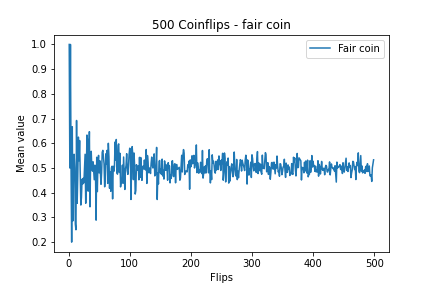
\includegraphics[width=4in]{img/05_1/fair_coinflip.png}
	\caption[Fair Coinflip]
	{A simulated fair coin flip, with 500 iterations of either \textit{heads} (1) or \textit{tails} (0). }
\end{figure}
If we repeat the experiment with an unfair coin instead, our assumption of a fair coin will now still lead us to assume the probabilities for \textit{heads} and \textit{tails} were $0.5$, just like in a perfect system. Here we are still assuming that if we observe enough events, the probabilities should be verified by the experiment. Statistical uncertainty in observing a fair coin could shift the observed probabilities for a while, but will always converge. Only after observing many events, we would start to question the assumptions we had at the beginning, e.g. of the coin being fair, because convergence is slow. 
\begin{figure}[h!]%Coinflip Comparison fair and unfair coin
	\centering
	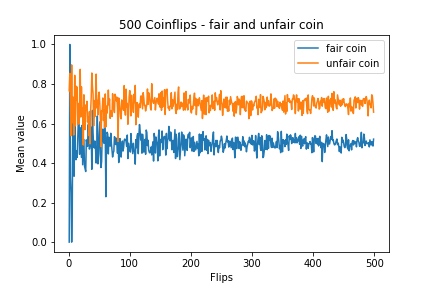
\includegraphics[width=4in]{img/05_1/unfair_coinflip.png}
	\caption[Fair and unfair coinflip comparison]
	{A simulated fair coin flip (blue) compared to the unfair coin flip (orange). Even though both tend towards different values for large sample sizes, in the first few flips, it is very hard to distinguish which coin is fair. Experimental conditions are the same as with the simulated fair coin flip.}
\end{figure}
So, from the frequentists perspective, if we were in the situation of playing coinflip with an unkown coin, it would take a long time, until we would accept the possibility that our model could be wrong. This inherent trust into the models is therefore used mostly in fields like physics, where the theory is assumed to reflect the ground truth no matter what, with the assumption that constants are always constant and the set of rules never changes, independent of where you are in the universe. This is called the Noether theorem, but since it only applies to the set of rules in physics, where controlling variables can be enforced with great precision, other fields need a more flexible theory to determine the probability of an event. So, assuming there are variables influencing our system in ways we cannot foresee with absolute precision, we need to be able to update the expected probabilities as a function of our observations. Since the probabilities are a crucial part of the model we applied to reality in the first place, we need to find a model that can be updated each time an observation took place. Bayesian statistics allows us to update our beliefs along the way. It dates back to Thomas Bayes, who in his essay "\textit{An essay towards solving a problem in the doctrine of chances}" [xxx] introduced the first version of this idea. Our percieved reality can always be flawed, not limited to a fair or unfair coin, but models for reality of all sorts can have intrinsic flaws, that can be quantified using this method of determining probabilities and updating models, along the way. Through this, probabilities become dependent on believability and credibility, confidence in decisions or environmental variables of the problem. Creating a model in bayesian statistics also allows for a causal bias introduced into the model, before observations even took place. So, if for example you would consider playing against someone with a coin you do not yet know to be fair, it is best to assume the coin is unfair at first. Noticing that a coin is unfair faster, and with higher probability, to update the model is valuable information. Previously we noticed, that the flexibility of bayesian models allow us to take into account environmental variables, but how many of those will actually lead to better predictions from the model? Occams Razor (xxx) is a good rule to follow, which would roughly translate to "\textit{choose a model as complicated as necessary but no more than that}". Or, in other words, a more complex model with more hyperparameters will in the end lead to better explanation ("a better fit") of the observed data, but prediction power will intrinsically decrease along the way, due to more noise being learned as a feature. 
\label{sec:introduction}
\cleardoubleoddpage

\subsection{Bayesian Statistics}
Models using the bayesian framework of statistics rely on conditional probability. These probabilities are conditioned on previous assumptions about the general environment. This can be surroundings, game states, environmental variables, etc. Since the properties of complex systems are majorly influenced by these traits, incorporating them into the model is of utmost importance. The general case of Bayes rule combines prior knowledge of the model, called a prior probability, with the observed evidence and its likelihood to form the posterior probability. The posterior probability can be interpreted as the probability of observing a certain set of observations dependent on the likelihood of the observations, given the model. 
\begin{equation}%Bayes Rule
	P(A|B) = \frac{P(B|A) P(A)}{P(B)}
\label{Bayes Rule for probabilities. }
\end{equation}
Here, A is the proposition and B the evidence, and we try to get the posterior $P(A|B)$, the degree of belief in $A$ if we have accounted $B$ to be true. $P(A)$ is the prior, the initial belief in $A$, while $P(B)$ is the likelihood of the evidence being true. This rule currently applies only to probabilities, but it can just as well be scaled up to probability distributions.
\begin{equation}%Bayes rule distributions
	p(A|B) = \frac{p(B|A) p(A)}{p(B)}
\label{Bayes Rule for probability distributions. }
\end{equation}
Probability distributions, which are factors defining models, can be tested for reliability via Bayes rule too. Also using Bayes rule, we can test our model assumptions and compare models. 
\begin{equation}%Bayes Rule Models and Data
	p(M|D,I) = \frac{p(D|M,I) p(M|I)}{p(D|I)}
\label{Bayes Rule for Model Comparison}
\end{equation}
Here, $M$ is the model in question, while $D$ is the observed Data, and $I$ is the previously known information of the system. We can then formulate a hierarchical Bayesian workflow.
\begin{enumerate}%Bayesian Workflow
	\item Use Bayes Rule to construct a naive model using only prior knowledge
	\item Update knowledge inside naive model 
	\item Create more complex model using Bayes rule for models
	\item Update knowledge about complex model
	\item repeat steps 1-4 until KL-Divergence converges to 0.
\end{enumerate}
%When we maximize the likelihood trough the Maximum Likelihood Method, we can approximate the true parameters through the model parameters. [xxx]
Every bit of knowledge we have about the system is now encoded in probability distributions, but to calculate this workflow, we need some class of probability distributions, that is sensible to use in most models, and which can preferrably be solved analytically. In experiments, we will see that this workflow is not as easy as expected, since the evidence is often intractable (xxx look up from VB Wikipedia), which then can only be evaluated approximately. Also, we need to take into account, that the total solution space of Bayesian priors may not contain the solution we try to achieve, because the true model may be something very different, from what we originally thought it was. Here Occams Razor is again the doctrine we use to make decisions about model choice: Our model shall be complicated enough to grasp the underlying dynamic, but needs to be naive enough to not learn noise as a feature. This leads to Gaussian processes, since they have a lot of convenient properties. The priors of Gaussian Processes ($\mathcal{GP}$) are appropriate and have infinite basis functions. These are flexible enough for nonlinear models, but still retain analytic solutions. Through this, they are especially computationally feasible. Also, Student-\textit{t}-processes, as they are scaled Gaussian processes, seem to be a logical choice. Even though they are more restrained in the amount of computation tasks that can be done analytically, compared to the Gaussian Processes. 

%prior VB section
In applications of the Bayes rule there are posterior terms containing the information about the data, but sometimes they have combinatorially large search spaces. This leads to the intractability of these terms, represented by $\int_X P(Y,X)dX$.
\begin{equation}%Bayes with intractable term
	P(X|Y) = \frac{P(Y|X)P(X)}{P(Y)} = \frac{P(Y|X)P(X)}{\int_Z P(Y,X)dX}
	\label{eq:Bayes_with_intractable_term}
\end{equation}
To obtain the approximation using Variational Bayes, we introduce a variational distribution. 
\begin{equation}%Variational Distribution
	Q(X) \approx P(X|Y)
	\label{eq: Variational Distribution}
\end{equation}
This distribution $Q(X)$ is restricted to be of a family of simpler distributions than the true distribution, e.g. a posterior, $P(X|Y)$. The distribution family is selected with the intention of finding a $Q(X)$ similarly enough to $P(X|Y)$ so that $Q(X)$ can be used instead of $P(X|Y)$. We use KL-divergence to measure the dissimilarity of the distributions, but with a slight variation. Instead of using a KL-version $D_{KL}(p|q)$ that is applied in the expectation propagation algorithm, we use the reverse KL-divergence. 
\begin{equation}%Expectation maximisation KL-Divergence
	D_{KL}(Q|P) \triangleq \sum_{X} Q(X) \log \frac{Q(X)}{P(X|Y)}
	\label{eq: Expectation maximisation KL-Divergence}
\end{equation}
given, that
\begin{equation}%ELBO Intro
	P(X|Y) = \frac{P(Y,X)}{P(Y)},
	\label{eq: ELBO Intro}
\end{equation}
the KL Divergence here can be rewritten as
\begin{subequations}%new KL for ELBO
	\label{eq:new_KL_ELBO}
	\begin{align}
		D_{KL}(Q|P) = \sum_{X}Q(X) \Big[\log \frac{Q(X)}{P(X,Y)}+\log P(Y)\Big]  \\
		= \sum_{X}Q(X) [\log Q(X) - \log P(X,Y)] + \sum_{X}Q(X)[\log P(Y)]. 
	\end{align}
\end{subequations}
After seeing that $P(Y)$ is constant with respect to $X$ and $\sum_{X}Q(X)=1$ because $Q(X)$ is a distribution, and rewritten with the definition of the expected value for a discrete random variable, we arrive at
\begin{equation}%evidence log
	\log P(Y) = D_{KL}(Q|P) - \mathbb{E}_X[\log Q(Y) - \log P(X,Y)] = D_{KL}(Q|P) + \mathcal{L}(Q)
	\label{eq:evidence_log}
\end{equation} 
Since $P(Y)$ is fixed under $Q$, maximizing $\mathcal{L}(Q)$ minimizes the KL Divergence from Q to P. $\mathcal{L}(Q)$ is also known as the Evidence Lower Bound, which will be important to the evaluation of models later on. The variational distribution is usually assumed to factorize over some partition of the latent Variables $X$. 
\begin{equation}%Variational Distribution Factorisation
	Q(X) = \prod_{i=1}^{M} q_i(X_i)
	\label{eq: Variational Distribution Factorisation}
\end{equation}
Using Variational Calculus we find that the best distribution in a Bayesian workflow with Variational Bayes is
\begin{equation}%VB best Distribution
	q_j^* (X_j|Y) = \frac{\exp(\mathbb{E}_{i\neq j}[\ln p(X,Y)])}{\int \exp(\mathbb{E}_{i\neq j}[\ln p(X,Y)]) dZ_j},
	\label{eq: VB best Distribution}
\end{equation}
where $\mathbb{E}_{i\neq j}[\ln p(X,Y)]$ is the expectation value of the logarithm of the joint probability of data and latent variables not in the partition. Due to circular depencies between the parameters, the evaluation of these in a program offers to be solved iteratively. With this, due to the type of the distribution $Q(X)$, an analytical approximation for the posterior probability can be achieved, allowing the iterative calculation of parameters of the model. Variational Bayes can be used out of the box. Stan provides an implementation known as Automatic Differentiation Variational Inference (ADVI, Kucukelbir) that approximates the posterior with a Gaussian as the variational approximation. For more details, see section \ref{sec:stochastic_gradient_ascent}.
\label{sec:bayes}
\cleardoubleoddpage

\subsection{Gaussian Processes}
Supervised Learning Machine Learning can be divided into two classes of problems, regression and classification. Where in Classification the machine learning algorithm should decide between discrete class labels, the output of a regression algorithm is usually a continuous quantity. Due to the nature of the Gaussian Processes suiting regression problems, a focus is put on these, even though Gaussian Processes can also solve classification problems \cite{Rasmussen_06}. There are several ways of interpreting a Gaussian process, the function space view, and the weight-space view. In the weigth space view, the Gaussian Process is pictured as a process, with infinity many basis functions with corresponding weights. In the function space view, the gaussian process is a distribution over functions, and inference takes place in the function space defined by the process. The Gaussian process, as mentioned in section \ref{sec:capm} and \ref{sec:apt}, is mainly used to find the covariance matrices, that encode the covariance structure of the problem. 

\subsubsection{Weight Space View}
A simple Gaussian process will be derived here. Starting with a standard linear regression model with Gaussian noise
\begin{subequations}%Linear Regression Gaussian
	\label{eq:Linear Regression Model}
	\begin{align}
	f(x) = \bm{x}^\top \bm{w}         \label{eq: linear regression function} \\
	y = f(\bm{x}) + \epsilon         \label{eq: observed target value} \\
	\epsilon \thicksim \mathcal{N}(0, \sigma_{n}^{2})
	\end{align}
\end{subequations}
Here $\bm{x}$ is the input vector, $\bm{w}$ is the vector containing the weigths, $f$ is the function value and $y$ the observed target value. Also, $\epsilon$ is the independent noise, and it follows an independent, identically distributed Gaussian distribution with zero mean and variance $\sigma_{n}^{2}$. The likelihood, as probability density of observations given parameters factors over the cases of the training set. 
\begin{subequations}%Likelihood in Weight Space View
	\label{eq:Likelihood Weight Space View}
	\begin{align}
	p(\bm{y}|X,\bm{w}) = \prod_{i=1}^{n} p(y_i|\bm{x}_{i}, \bm{w}) =  \prod_{i=1}^{n} \frac{1}{\sqrt{2\pi}\sigma_{n}} \exp \Big( -\frac{(y_i -\bm{x}_{i}^{\top}\bm{w})^2}{2\sigma^2_n}\Big)      \label{eq:likelihood wieght space 1} \\
	= \frac{1}{(2\pi\sigma_n^2)^{n/2}} \exp \Big( -\frac{1}{2\sigma_n^2 }|\bm{y}-X^{\top}\bm{w}|^2 \Big) = \mathcal{N}(X^{\top}\bm{w}, \sigma_n^2 I)         \label{eq:likelihood weight space 2}.
	\end{align}
\end{subequations}
$X$ is all the data points from the input, and $|x|$ stands for the euclidian length of a vector $x$. Also, a prior must be specified, containing our beliefs about the parameters before observing the input. Therefore, we will distribute the weights using a zero mean Gaussian prior with covariance matrix $\Sigma_p$, 
\begin{equation}%Weights Distribution
	\bm{w} \thicksim \mathcal{N}(\bm{0}, \Sigma_p).
\label{Distribution of weights using a zero mean Gaussian with covariance matrix.}
\end{equation}
To apply Bayes rule, we need a marginal likelihood, which acts as a normalizing constant, and is independent of the weights by integrating them out. 
\begin{equation}%marginal likelihood
	p(\bm{y}|X) = \int p(\bm{y}|X,\bm{w}) p(\bm{w}) d\bm{w}
\label{eq: Marginal likelihood as normalizing constant}
\end{equation}
The full Bayes rule in this case then becomes the following
\begin{equation}%Bayes Rule for Linear Regression
	p(\bm{w}|\bm{y},X) = \frac{p(\bm{y}|X,\bm{w})p(\bm{w})}{p(\bm{y}|X)}
\label{Bayes Rule for linear Regression}
\end{equation}
Using complete the square and ignoring the marginal likelihood, we find
\begin{equation}%unnormalized posterior
	p(\bm{w}|X,\bm{y}) \thicksim \mathcal{N}(\frac{1}{\sigma_n^2}(\frac{1}{\sigma_n^2}XX^{\top}+ \Sigma_p^{-1}), (\frac{1}{\sigma_n^2}XX^{\top}+ \Sigma_p^{-1})^{-1})
\label{Unnormalized posterior}
\end{equation}
With this, we can easily find the predictive distribution for $f_* \triangleq f(\bm{x}_*)$, by averaging the output of all possible linear models with respect to the Gaussian posterior,
\begin{subequations}%Gaussian posterior predictive distribution
	\label{eq:Gaussian posterior predictive distribution}
	\begin{align}
		p(f_*|\bm{x}_*,X,\bm{y}) = \int p(f_*|\bm{x}_*, \bm{w})p(\bm{w}|X,\bm{y}) d\bm{w}    \label{eq:predictive distribution 1} \\
		= \mathcal{N}(\frac{1}{\sigma_n^2}\bm{x}_*^{\top}(\frac{1}{\sigma_n^2}XX^{\top}+ \Sigma_p^{-1})^{-1}X\bm{y}, \bm{x}_*^{\top}(\frac{1}{\sigma_n^2}XX^{\top}+ \Sigma_p^{-1})^{-1}\bm{x}_*).         \label{eq: predicitve distribution 2}
	\end{align}
\end{subequations}
This model can easily be expanded by transforming the input into some high dimensional space using a set of basis functions and subsequently applying the linear model in this higher dimensional space. Applying the map $\phi(x) = (1,x,x^2,x^3,x^4,...)^{\top}$ would for example implement polynomial regression, during which a $D$-dimensional input vector $x$ is mapped into an $N$-dimensional feature space. This allows us to rewrite the model as
\begin{subequations}%Feature Space Gaussian process
	\label{eq:Feature Space Gaussian process}
	\begin{align}
	f(\bm{x}) = \phi(\bm{x})^{\top} \bm{w}         \label{eq: feature space model} \\
	f_*|\bm{x}_*,X,\bm{y}  \thicksim \mathcal{N}\Big( \frac{1}{\sigma_n^2}\phi(\bm{x}_*)^{\top}(\sigma_n^{-2}\Phi \Phi^{\top} + \Sigma_p^{-1})^{-1} \Phi \bm{y} , \label{eq: predictive distribution mean} \\
	 \phi(\bm{x}^{\top})(\sigma_n^{-2}\Phi \Phi^{\top} + \Sigma_p^{-1})^{-1} \phi(\bm{x}_*) \Big)        \label{eq: predictive distribution covariance} 
	\end{align}
\end{subequations}
where $\Phi(X)$ is the aggregation of all columns $\phi(\bm{x})$ for all cases in the data set in the transformed space. It presents a computational time benchmark when executing such a model, since the inversion of $N\times N$ matrices is of $\mathcal{O}(N^3)$ complexity. With high-dimensional feature spaces, reducing the argument of the complexity function is valuable. So, sometimes rewriting the equations as
\begin{equation}%rewritten Feature Space Gaussian Process evaluated in data space. 
	f_*|\bm{x}_*,X,\bm{y} \thicksim \mathcal{N}\Big( \phi_*^{\top}\Sigma_p\Phi(K+ \sigma_n^2 I)^{-1}\bm{y}, \phi_*^{\top} \Sigma_p \phi_* - \phi_*^{\top} \Sigma_p \phi_*(K+ \sigma_n^2 I)^{-1}\phi_*^{\top} \Sigma_p \phi_* \Big)
\label{Rewritten Feature Space Gaussian Process evaluated in data space.}
\end{equation}
is useful, since the complexity $\mathcal{O}(n^3)$ is the maximum complexity possible for $n$ datapoints \cite{Rasmussen_06}. Then, the kernel function $k(\bm{x},\bm{x'}) = k(\cdot , \cdot) = \phi_*^{\top} \Sigma_p \phi_*$ is easily identified. The kernel is often also called covariance function. \newline

\subsubsection{Function Space View}
This derivation can also be done in function space. Here, we can define a Gaussian Process as a collection of random variables, any finite number of which have a joint Gaussian distribution. Since a Gaussian process is solely defined by its mean and kernel function, it can be written as
\begin{subequations}%Gaussian process function space view
	\label{eq:Gaussian_process_function_space_view}
	\begin{align}
	m(x) =\mathbb{E}[f(x)]         \label{eq:function space view mean} \\
	k(\bm{x},\bm{x'}) = \mathbb{E}[(f(\bm{x})-m(\bm{x}))(f(\bm{x'})-m(\bm{x'})))]         \label{eq:function space view covariance function} \\
	f(x) \thicksim \mathcal{GP}(m(\bm{x}), k(\bm{x}, \bm{x'})).               \label{fuinction space view gaussian process}
	\end{align}
\end{subequations}
The Function space view notation will be the notation further on used in this thesis. Here, $\mathcal{GP}$ stands for a Gaussian Process, $m(\bm{x})$ is the mean function, and $k(\bm{x}, \bm{x'})$ is the kernel function. The consistency requirement, also marginalization property, states, that for a $\mathcal{N}$ $(y_a, y_b) \thicksim \mathcal{N}(\bm{\mu}, \Sigma)$ with general mean vector $\bm{\mu} = (m(\bm{x}_a), m(\bm{x}_b))^{\top}$ and covariance matrix $\Sigma$, the underlying $\mathcal{N}(y_a)$ is specified by $y_a \thicksim \mathcal{N}(\mu_a, \Sigma_{aa})$. $\Sigma_{aa}$ then is the submatrix of $\Sigma$ relevant to the distribution for $y_a$. Since the submatrixes are not intertwined in $\Sigma$, the examination of a larger set of variables does not change the distribution of a subset. Using the previously discussed linear regression model $f(x) = \phi(\bm{x})\bm{w}^{\top}$ with a gaussian prior on $\bm{w}$ we have mean and covariance
\begin{subequations}%Function space view linear regression mean and covariance
	\label{eq:Function space view linear regression mean and covariance}
	\begin{align}
	\mathbb{E}[f(\bm{x})] = \phi(\bm{x})^{\top} \mathbb{E}[\bm{w}] = 0         \label{eq:function space linear mean} \\
	\mathbb{E}[f(\bm{x})f(\bm{x'})] = \phi(\bm{x})^{\top} \mathbb{E}[\bm{w}\bm{w}^{\top}]\phi(\bm{x}) = \phi(\bm{x})^{\top}\Sigma_p\phi(\bm{x'}).         \label{eq:function space linear covariance}
	\end{align}
\end{subequations}
Given a kernel function, we can generate a random sample from a GP with Covariance matrix $K(X_*, X_*)$, where $X_*$ is the matrix containing all input points. 
\begin{equation}%Random Gaussian prior samples
	\bm{f_*} \thicksim \mathcal{N}(\bm{0}, K(X_*, X_*))
\label{Random Gaussian vector}
\end{equation}
The most used kernel function is the squared exponential,
\begin{equation}%squared exponential
	k_{sqe}(\bm{x_i}, \bm{x_j}) = exp(-\frac{1}{2l^2}d_{ij}^2).
	\label{eq:squared-exponential}
\end{equation}
Incorporating the knowledge of the training data for noise free predictions then leads us to
\begin{equation}%Joint Distribution according to prior
	\begin{bmatrix}	\bm{f} \\ \bm{f_*} \end{bmatrix} \thicksim \mathcal{N} \Bigg(0, \begin{bmatrix} K(X,X) & K(X,X_*) \\ K(X_*,X) & K(X_*,X_*) \end{bmatrix} \Bigg),
\label{eq:joint_distribution_according_to_prior}
\end{equation}
where now all variables without $_*$ are training variables, and all variables with $_*$ are the respective test variables. This gives 
\begin{equation}%conditioned/joint Gaussian prior
	\bm{f}_*|X_*,X,\bm{f} \thicksim \mathcal{N}(K(X_*,X)K(X,X)\bm{f}, K(X_*,X_*)-K(X_*,X)K(X,X)^{-1}K(X,X_*))
\label{conditioned/joint Gaussian prior}
\end{equation}
for the conditioned, joint Gaussian prior distribution on observations. Extending the model to incorporate noise on the data, we find
\begin{equation}%Joint Gaussian distribution according to prior with noise
	\begin{bmatrix}	\bm{y} \\ \bm{f_*} \end{bmatrix} 
	\thicksim \mathcal{N} \Bigg(0, 
	\begin{bmatrix} K(X,X)+\sigma_n^2 I & K(X,X_*) \\ K(X_*,X) & K(X_*,X_*) \end{bmatrix} \Bigg),
\label{eq:joint_gaussian_distribution_according_to_prior_with_noise}
\end{equation}
where the key predictive equations for Gaussian process regression are
\begin{subequations}%Key predictive equations for Gaussian process regression
	\label{eq: Key predictive equations for Gaussian process regression}
	\begin{align}
	\bm{f}_*|X,\bm{y},X \thicksim \mathcal{N}(\overline{\bm{f}_*}, cov(\bm{f}_*)),         \nonumber \\
	\overline{\bm{f}_*} \triangleq \mathbb{E}[\bm{f}_*|X,\bm{y},X_*] = K(X_*,X)[K(X,X) + \sigma_n^2 I]^{-1}\bm{y},        \nonumber \\
	cov(\bm{f_*}) = K(X_*,X_*) - K(X_*,X)[K(X,X)+ \sigma_n^2 I]^{-1}K(X,X_*).       
	\end{align}
	\label{eq:Key_predictive_equations_for_GP_reg}
\end{subequations}
Introducing the marginal likelihood $p(\bm{y}|X)$ again, we find
\begin{equation}%Marginal Likelihood function space view
	p(\bm{y}|X) = \int p(\bm{y}|\bm{f},X) p(\bm{f}|X) d\bm{f}.
\label{eq:marginal_likelihood_function_space_view}
\end{equation}
Solving this integral analytically it results to
\begin{equation}%Log Marginal likelihood
	log \Big(p(\bm{y}|X)\Big) = -\frac{1}{2}\bm{y}^{\top}(K+ \sigma_n^2 I)^{-1}\bm{y} -\frac{1}{2}log|K+ \sigma_n^2 I| - \frac{n}{2}log ( 2\pi).
\label{eq:Log_marginal_likelihood}
\end{equation}
Using this, we have derived the regular Gaussian process. It is easy to see, that iterative usage of the learning equations (previously: key predictive equations) is the same as learning from all data points at once due to the marginalization property. The following figures provide an example. At first, we introduce random prior samples  in figure \ref{fig:prior_squ_exp}, specified by a squared exponential kernel centered around a mean of 0 and with a covariance of 2. 
\begin{figure}[h!]%prior example squared exponential
	\centering
	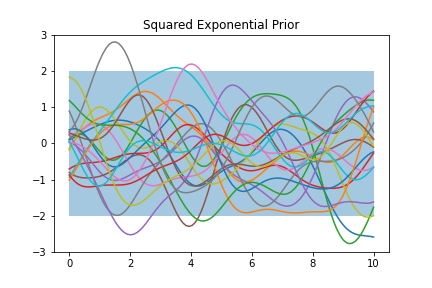
\includegraphics[width=4in]{img/05_3/gp_prior.png}
	\caption[GP prior samples]
	{Samples from a Gaussian Process prior with a squared exponential kernel. To add to the draws, the 95\% confidence interval is highlighted with a blue background. }
	\label{fig:prior_squ_exp}
\end{figure}
Then, we introduce data points, which were randomly generated using a modified sine function with added gaussian noise, see figure \ref{fig:generated_data}. 
\begin{figure}[h!]%data points to train on
	\centering
	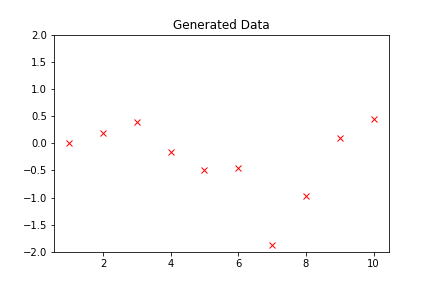
\includegraphics[width=4in]{img/05_3/generated_data.png}
	\caption[Random data from sine function with Gaussian noise]
	{Data generated from a sine function with added Gaussian noise.}
	\label{fig:generated_data}
\end{figure}
Using the learning equations \ref{eq:Key_predictive_equations_for_GP_reg}, we can train a Gaussian process on the data points and find the following posterior samples, see figure \ref{fig:GP_sqexp_samples} and confidence intervals, having solved the Gaussian Process. 
\begin{figure}[h!]
	\centering
	\begin{minipage}{0.45\textwidth}
		\centering
		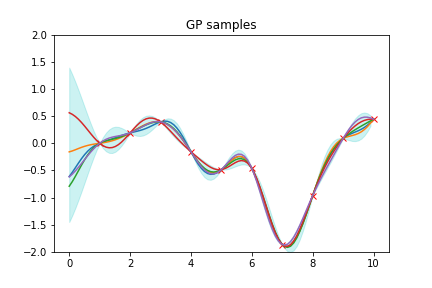
\includegraphics[scale=0.6]{img/05_3/gp_samples.png} % first figure itself
		\caption[Trained GP samples with covariance interval]{The GP conditioned on the generated dataset, with the 95\% confidence interval and 5 samples drawn from the GP. }
		\label{fig:GP_sqexp_samples}
	\end{minipage}\hfill
	\begin{minipage}{0.45\textwidth}
		\centering
		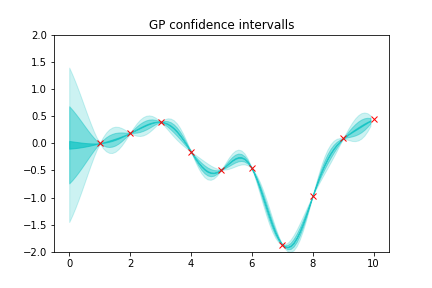
\includegraphics[scale=0.6]{img/05_3/gp_confints.png} % second figure itself
		\caption[Trained GP with covariance intervals]{The GP conditioned on the generated dataset, with confidence intervals drawn into the graph as blue shading. }
		\label{fig:GP_confidence_intervals}
	\end{minipage}
\end{figure}
The confidence intervals in figure \ref{fig:GP_confidence_intervals} have 1, 2, and 3 $\sigma$. This depiction also highlights the interpretation of GP predictions as probability distributions. \newpage
\label{sec:gp}
\cleardoubleoddpage

\subsection{Gaussian Kernel Functions}
A covariance function, or kernel function is a key part of the model used. Since not any function linking two inputs $x$ and $x'$ will in general be a viable kernel function, necessary, as well as useful properties of kernel functions need to be discussed. First, kernel functions must be positive semidefinite, 
\begin{equation}%positive semidefiniteness of kernel functions
	\int k(\bm{x},\bm{x'})f(\bm{x})f(\bm{x'})d\mu(\bm{x})d\mu(\bm{x'}) \geq 0.
\label{eq:positive_semidefiniteness_of_kernel_functions}
\end{equation}
Here, $\mu$ denotes a respective measure. Kernel functions also can be stationary, when it is a function of $\bm{x} - \bm{x'}$, exhibiting translation invariance in input space. A kernel function can be isotropic, a function of $|\bm{x} - \bm{x'}|$, making it invariant to all rigid motions. Isotropic kernel functions are also known as radial basis functions (RBF). If the kernel function is a function of $\bm{x} \cdot \bm{x'}$, it is called a dot-product kernel function. These are invariant to a rotation of coordinates about the origin, but not translation. Kernel functions also are the underlying reason for some properties concerning the total process, e.g. mean-square continuity and differentiability. \newline
\textbf{Continuity:} Continuity is a property of the Gaussian process, directly exhibited from the choice of kernel function. A stochastic process is continuous, if in a sequence of points $x_1, x_2, ..$ with another fixed point $_x*$ in $\mathbb{R}^D$ $|\bm{x}_k - \bm{x}_*| \to 0$ as $k \to \infty$. Then a process $f(x)$ is continuous in mean-square at $x_*$ if $\mathbb{E}[|f(x_k)-f(x_*)|^2] \to 0$, as $k \to \infty$. If this holds for all $x_* \in A$ where $A$ is a subset of $\mathbb{R}^D$, then $f(x)$ is said to be continuous in mean square over $A$. A random field is continuous in mean square if and only if its covariance function is continuous at $x=x_*=x'$. 
For stationary covariance funtions this reduces to checking continuity at $k(0)$. \newline
\textbf{Differentiability:} Using the mean square derivative of $f(x)$ in \textit{i}th direction 
\begin{equation}%mean square derivative of i-th direction
	\frac{\partial f(x)}{\partial x_i} = \lim_{h \to 0} \frac{f(x+h\bm{e}_i)-f(x)}{h},
\label{eq:mean_square_derivative_of_i-th_direction}
\end{equation}
and checking if the limit exists for order $2k$ and is finite at $x=0$, then the \textit{k}th order limit exists as a mean square limit. Here, the properties of the kernel around $0$ determine the smoothness properties of a stationary process. \newline \newline
Following, some of the more prominent kernel functions are presented, with some practical properties. Almost all of the following are stationary and non-degenerate, meaning they are stationary and of infinite rank.\newline
\begin{equation}%linear kernel function
	k_{linear}(\bm{x_i}, \bm{x_j}) = \sigma^2 \bm{x_i}^{\top} \cdot \bm{x_j} 
\label{eq:linear_kernel_function}
\end{equation}
is the linear kernel. As the most simple of kernels, it is as an exceptional case in this listing neither stationary, nor non-degenerate. 
\begin{equation}%exponential kernel function
	k_{exp}(\bm{x_i}, \bm{x_j}) = exp(-\frac{1}{2l}d_{ij}),
\label{eq:exponential_kernel_function}
\end{equation}
the exponential kernel, where $d_{ij} = ||\bm{x}_i - \bm{x}_j||_2$ is the Euclidian distance between the input arguments. 
\begin{equation}%squared exponential kernel
	k_{sqe}(\bm{x_i}, \bm{x_j}) = exp(-\frac{1}{2l^2}d_{ij}^2)
\label{eq:squared_exponential_kernel}
\end{equation}
is the squared exponential kernel. It is also known as radial basis function. 
\begin{equation}%matern 32 kernel
	k_{mat32}(\bm{x_i}, \bm{x_j}) = \Bigg( 1 + \frac{\sqrt{3}d_{ij}}{l} \Bigg) exp \Bigg( - \frac{\sqrt{3}}{2l} d_{ij} \Bigg)
\label{eq:matern_32_kernel}
\end{equation}
is the Matern3/2 kernel. it is a special case like the Matern5/2 kernel
\begin{equation}%matern 52 kernel
	k_{mat52} = \Bigg( 1+ \frac{\sqrt{5}d_{ij}}{l} + \frac{5r^2}{3l^2} \Bigg)exp\Bigg( \frac{\sqrt{5}d_{ij}}{l} \Bigg)
\label{eq:matern_52_kernel}
\end{equation}
of the Matern class of kernels
\begin{equation}%matern kernel class
	k_{mat} = \frac{2^{1-\nu}}{\Gamma(\nu)} \Big( \frac{\sqrt{2\nu}d_{ij}}{l} \Big)^\nu K_\nu \Big( \frac{\sqrt{2 \nu}d_{ij}}{l} \Big) .
\label{eq:matern_kernel_class}
\end{equation}
The matern kernels can be constructed with positive parameter $\nu$, $K_\nu$ is a modified Bessel function. Also, as $\nu \to \infty$ the function becomes the smooth squared exponential kernel, for $\nu = 1/2$ the Matern class kernel becomes the Ornstein-Uhlenbeck kernel. This kernel gives rise to a continuous-time AR(p) Gaussian process. But since this kernel was not used in the further work, it will not be discussed more. Kernel functions are used to calculate the entries of the covariance matrices. Different kernel functions apply better or worse to different problems. Even though there sometimes are kernel function choices that seem more applicable to a problem from prior assumptions, different kernel functions should be used and compared to ensure better models. 
\newline \newline
On another note, novel kernels can be created through different methods, for example by combining different existing kernels. Since kernels are always independent, kernels can be added to create a new kernel. For the same reason the multiplication of two kernels also produces a new kernel. In addition, new kernels can be created using rescaling, where kernels are e.g. normalized, or through convolution, where the kernels are mapped onto other spaces. Another major part of the properties of kernel functions are hyperparameters. These influence for example the frequency of changes exhibited by a kernel function. This hyperparameter, usually denoted as $l$ is often called kernel lengthscale. An example, of how this parameter influences the model is shown in figure \ref{fig:lengthscale}.
\begin{figure}%lengthscale
	\label{fig:lengthscale}
	\centering
	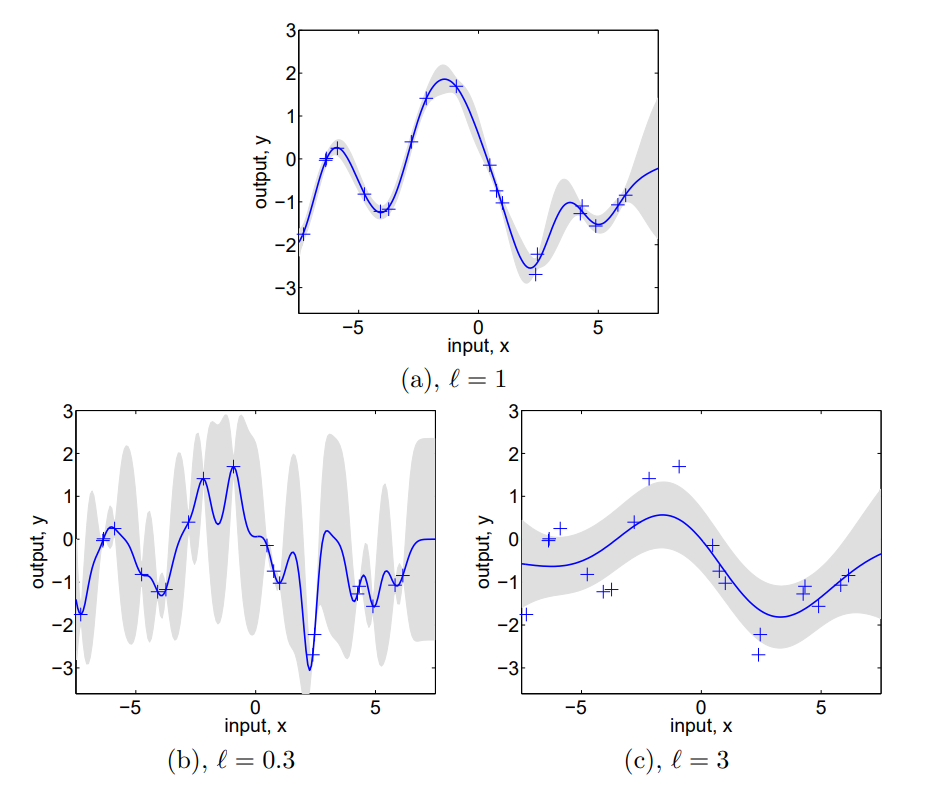
\includegraphics[width=4in]{img/05_4/lengthscale.png}
	\caption[Lengthscale influence on samples]
	{Comparison of hyperparameters for the squared exponential kernel function. A large lengthscale exhibits properties where the function does not react to changes quickly, while a small lengthscale gives the opportunity to react to changes almost immediately. While small lengthscales usually lead to better fits, the prediction power often decreases since more information from noise is incorporated into the covariance matrix. The data is generated from a GP with $l_a=0.3$, $l_b=1$, $l_c=3$, $\sigma_f=1$, and $\sigma_n=0.1$ \cite{Rasmussen_06}. The panel a has lengthscale $l_a$, panel b has lengthscale $l_b$, and panel c $l_c$.}
\end{figure}
The variances, often denoted by $\sigma_n$ for the noise variance, and $\sigma_f$ for the kernel function variance, influence the confidence interval in which we assume the functions to lie. $\sigma_n$ stems from the noise we attribute to the special systemic noise of the problem at hand, while $\sigma_f$ stems from just observing data that is noisy. A large noise variance and kernel variance will exhibit the kernel matrix incorporating a larger error tolerance. This can be seen in the enlargening of the confidence intervals on the draws of functions from the same process. Higher Variances lead to more flexible fitting, while lower variances will be more rigid. On the other hand, if variances are too high or too low, essential information about the structure of the problem can get lost.
\label{sec:kernels}
\cleardoubleoddpage

\section{Gaussian Process Latent Variable Models}
Latent variables are variables of an experiment or theory, that influence the outcome of an experiment without being directly measurable. The only way to obtain a latent variable is to infer it from the information that can be observed in the experiment. Intelligence, for example, is a latent variable. It is not directly measurable, but is influencing the outcome of some experiments in psychology. While tests for intelligence try to measure intelligence by inferring it, they can only give a general direction of the true value, assuming it exists and can be ascertained to a single value in a controlled environment. The test then tries to measure what we believe to be components of intelligence, e.g. skills in logic, pattern recognition and grammar. The measured scores are then used to calculate an overall score, which we believe to be a measure for intelligence. While latent variable models, such as the one used in psychology to infer intelligence from a test, enable scientists to more accurately describe phenomena we already have a general understanding about, the models also enable us to infer data in other fields. Since latent variable models are already directly connected to statistics, it is not a far stretch to apply some of them in fields that previously used almost exclusively statistical methods to describe phenomena. Also, latent variable models could reveal relations between different variables of the system, if different variables are dependent on the same set of latent variables, and therefore change with a behaviour that can be infered by knowing the state of the latent variables. \newline
Assume that a data matrix $Y \in \mathbb{R}^{N\times D}$ is given and the goal is to find a lower dimensional representation $X \in \mathbb{R}^{N\times Q}$ of the matrix, without loosing a major share of the information encoded in the data matrix. Previous models have mostly used Principal Component Analysis (PCA) to achieve this dimensionality reduction. Principal Component Analysis has also been shown to be the maximum likelihood solution to a particular form of Gaussian Latent Variable Model \cite{Tipping_Bishop_1999_1}\cite{Tipping_Bishop_1999_2}. PCA here embeds $\mathcal{Y}$, the data space, via linear mapping into a latent space $\mathcal{X}$. Later on, the Gaussian Process Latent Variable Model was introduced as a non-linear extension to probabilistic PCA \cite{Lawrence_2005}. \newline \newline
Probabilistic PCA (P-PCA) is a model derived by using the probabilistic framework. While P-PCA facilitates statistical testing and Bayesian workflows, it can also be applied to problem sets, where PCA previously could not be used efficiently. This is especially the case for missing data in the dataset. Also, P-PCA can be represented as a general Gaussian density model, which can efficiently be solved through computing maximum likelihood estimates for the parameters associated with the covariance matrix from principal components. This promises effective classification and novelty detection. Starting with factor analysis, a linear relation between the observation vector $\bm{t} \in \mathbb{R}^d$ and the vector of latent variables $\bm{x} \in \mathbb{R}^q \text{, } d>q$ can be established like 
\begin{equation}%Factor analysis
	\bm{t} = W\bm{x} + \bm{\mu} + \bm{\epsilon}
\label{eq:Factor_Analysis}
\end{equation}
with noise $\bm{\epsilon} \sim \mathcal{N}(\bm{0, \Sigma})$ and mean vector $\bm{\mu}$ to permit the model with a non-zero mean. It promises a parsimonious explanation of dependencies between observations. If $\bm{x}$ is assumed to be standard Gaussian, we can find the distribution for $t$ 
\begin{equation}%factor analysis results
	\bm{t} \sim \mathcal{N}(\bm{\mu}, WW^{\top} + \Sigma).
\label{eq: Factor analysis results}
\end{equation}
Now, when constraining the covariance matrix $\Sigma$ to be a diagonal matrix, we will have only autocorrelation in observed variables (conditional independence), given the latent variables $\bm{x}$ and the mapping $W$. The latent variables are therefore used to explain correlations between observation variables. \newline
With this, we can find P-PCA by considering the $\bm{x}$-conditional probability distribution over $\bm{t}$-space
\begin{equation}%x-conditional probability dist over t-space
	\bm{t}|\bm{x} \sim \mathcal{N}(W\bm{x} + \bm{\mu}, \sigma^2I)
\label{eq: x-conditional probability dist over t-space}
\end{equation}
Integrating out the latent variables, we arrive at the Gaussian marginal distribution for $\bm{t}$
\begin{equation}%marginal distribution t
	\bm{t} \sim \mathcal{N}(\bm{\mu}, WW^{\top} + \sigma^2I)
\label{eq: marginal distribution t}
\end{equation}
with corresponding log-likelihood
\begin{equation}%log likelihood p-pca
	\log p(\bm{t}) = -\frac{N}{2} \Big(d \ln(2\pi) + \ln|WW^{\top} + \sigma^2I| + \text{tr}((WW^{\top} + \sigma^2I)^{-1}\frac{1}{N}\sum_{n=1}^{N}(\bm{t}_n - \bm{\mu})(\bm{t}_n - \bm{\mu})^{\top}) \Big).
\label{eq: log likelihood p-pca}
\end{equation}
Iterative maximisation of the log-likelihood now presents a fast and reliable way to optimise the P-PCA. From this model, standard PCA can be recovered when $\sigma^2 \to 0$ and $ WW^{\top} + \sigma^2I \to (W_{ML}^{\top}W_{ML})$. 
\newline \newline
Considering the GPLVM, we can find the generating procedure to be
\begin{equation}%generating procedure GPLVM
	Y_{n,:} = \bm{f}(X_{n,:}) + \bm{\epsilon}_n,
\label{eq: generating procedure GPLVM}
\end{equation} 
closely resembling the linear model of a GP, equation \ref{eq:Factor_Analysis} again. Here, $\bm{f} = f(f_1,...,f_D)$ is a group of $D$ independent samples from a Gaussian process $f_d \sim \mathcal{GP}(0, k(\cdot,\cdot))$. $X$ is the matrix containing the latent space ($\mathcal{X}$) positions.  Due to the structure of the problem at hand, the rows of the data matrix $Y$ are assumed to be jointly Gaussian distributed, while the columns are independent. This can be interpreted as every data point (return rate) of a single day being Gaussian distributed, while there is no time-dynamic. Each sample of $Y_{:,d} \sim \mathcal{N}(Y_{:,d}|\bm{0}, K)$ is assumed to incorporate noise inside the covariance matrix $K = k(X,X) + \sigma^2 I$, where $\sigma^2$ is the variance of the noise $\bm{\epsilon}$, which is assumed to be random. We find the marginal likelihood of $Y$ to be
\begin{equation}%marginal likelihood of data gplvm
	p(Y|X) = \prod_{d=1}^{D} \mathcal{N}(Y_{:,d}|\bm{0},K) = \frac{1}{(2\pi)^{ND/2}|K|^{D/2}} \exp \Bigg(-\frac{1}{2}tr(K^{-1}YY^{\top})\Bigg).
\label{eq: marginal likelihood of data gplvm}
\end{equation}
The covariance matrix $K$ gives the dependency on the kernel hyperparameters as well as the latent space positions $X$. Lawrence (2005) suggested to optimize the log-marginal-likelihood $\log p(Y|X)$, with the hyperparameters and latent space positions as the parameters used for optimisation. 
\label{sec:GPLVM}
\cleardoubleoddpage

\subsection{Student-t-Process}
An alternative to the Gaussian processes provide the Student-t-processes \cite{Shah_14}. They can be regarded as a generalized Gaussian process. Assuming an inverse Wishart prior for the kernel of a Gaussian process will result in a Student-t process. Due to this, we can also think of the Student-t process as a prior over functions, that is non-parametric. Also belonging to the family of elliptical processes, the Student-t process ($\mathcal{TP}$) offers more robustness to outliers inherent to the process, due to the broader flanks of the Student-t distribution. It is the most general elliptically symmetric process for which analytical marginal and predictive distributions exist. While some argue \cite{Shah_14}, that the predictive covariances of a Gaussian process do not depend on the training observations, the predictive covariances from a Student-t process do depend on training observations. Deriving the Student-t process, we will start with a Wishart process $W_n(\nu,K)$. The Wishart distribution is a distribution over the set of real-valued symmetric matrices, of size $n\times n$, that are positive definite $\Pi(n)$. The density function is
\begin{subequations}%Wishart distribution
	\label{eq:}
	\begin{align}
	\Sigma \sim W_n(\nu,K) \text{, if }         \label{eq:Wishart Distribution} \\
	p(\Sigma) = \Big(|K|^{\nu/2}2^{\nu n/2} \Gamma_n(\nu/2)\Big)^{-1}|\Sigma|^{(\nu-n-1)/2} exp \Big(-\frac{1}{2}tr(K^{-1}\Sigma)\Big)         \label{eq:Wishart distribution definition}
	\end{align}
\end{subequations}
with $\nu > n-1,\text{ } \nu \in \mathbb{R}_+$. This definition exhibits the marginalisation property, just like a GP. But since for $\nu \to \infty$ almost surely $\nu^{-1}\Sigma \to K$, thereby loosing the usefulness of the process. This property is not exhibited in the inverse Wishart process ($Iw_n(\nu, K)$) \cite{Dawid_1981}.
\begin{subequations}%Inverse Wishart Distribution
	\label{eq:}
	\begin{align}
	\Sigma \sim IW_n(\nu,K) \text{ if }         \label{eq:Inverse Wishart distribution} \\
	p(\Sigma) = \Big(\frac{|K|^{(\nu+n-1)/2}}{2^{(\nu+n-1)n/2}\Gamma_n((\nu+n-1)/2)}\Big)^{-1}|\Sigma|^{-(\nu+n-1)/2} exp \Big(-\frac{1}{2}tr(K\Sigma^{-1})\Big)         \label{eq:Inverse Wishart distribution definition}
	\end{align}
\end{subequations}
This formulation requires $\nu > 2$ and $\mathbb{E}[\Sigma] = (\nu-2)^{-1}K$, for the mean and the covariance to exist. Both Wishart distributions place prior mass on every possible matrix $\Sigma$ stemming from the set $\Pi(n)$. It was also previously shown, that the Inverse Wishart distribution is consistent under marginalization. Any submatrix $\Sigma_{11}$ will be $Iw_{n1}(\nu_1K-\Sigma_{11})$ distributed. With this, we can define a Inverse Wishart Process analogous to a Gaussian process with a base kernel $k:\mathcal{X} \times \mathcal{X}\to \mathbb{R}$
\begin{equation}%Inverse Wishart Process
	\sigma \sim \mathcal{IWP}(\nu,k(\cdot,\cdot)).
\label{eq: Inverse Wishart Process}
\end{equation}
If the Inverse Wishart process is applied as prior on the kernel function of a $\mathcal{GP}$, a Student-t process 
\begin{subequations}%Student-t process
	\label{eq:Student-t process}
	\begin{align}
	\sigma \sim \mathcal{IWP}(\nu,k_\theta)         \label{eq:inverse wishart covariance kernel} \\
	\bm{y}|\sigma \sim \mathcal{GP}(\mu, (\nu-2)\sigma)         \label{eq:hierarchical gaussian process with iwp kernel}
	\end{align}
\end{subequations}
generative approach is achieved. We find the data to be Student-t distributed if the density is of the structure
\begin{subequations}%student-t distributed data
	\label{eq:multivariate Student-t distributed data}
	\begin{align}
	\bm{y} \sim \mathcal{MVT}_n(\nu,\bm{\mu},K)         \label{eq:multivariate Student-t shorthand} \\
	p(\bm{y}) = \frac{\Gamma(\frac{\nu+n}{2})}{((\nu-2)\pi)^{\pi/2}\Gamma(\nu/2)}|K|^{-1/2}\Big(1+\frac{(\bm{y}-\bm{\mu})^{\top}K^{-1}(\bm{y}-\bm{\mu})}{\nu-2}\Big)^{-(\nu+n)/2} ,        \label{eq:multivariate Student-t distributed data def}
	\end{align}
\end{subequations}
for which the mean and covariance are given by
\begin{subequations}%mean and cov studt
	\label{eq:mean and cov studt}
	\begin{align}
	\mathbb{E}[\bm{y}] = \mathbb{E}[\mathbb{E}[\bm{y}|\Sigma]] = \bm{\mu}         \label{eq:mean studt} \\
	cov[\bm{y}] = \mathbb{E}[\mathbb{E}[(\bm{y}-\bm{\mu})(\bm{y}-\bm{\mu})^{\top}|\Sigma]]         \label{eq:cov studt}
	\end{align}
\end{subequations}
\cite{Shah_14}. The Student-t process is consistent under marginalisation. As a shorthand, we write $f \sim \mathcal{TP}(\nu, \bm{\mu},K)$ for a joint Student-t process over a finite collection of function values, as a similar counterpart to the Gaussian process over function values \ref{eq:Gaussian_process_function_space_view}. The student-t process generalizes the Gaussian process through the introduction of the degree of freedom parameter $\nu$. For  $\nu \to \infty$ we arrive at a Gaussian process, while at $\nu = 1$ we have a Cauchy process. Analyzing this hyperparameter, we find that it controls how much probability mass lies in the tails of a distribution, directly influencing how large of a variance samples from a Student-t process have compared to a Gaussian process.
\begin{figure}[h!]%Comparison GP and TP samples
	\centering
	\begin{minipage}{0.75\textwidth}
		\centering
		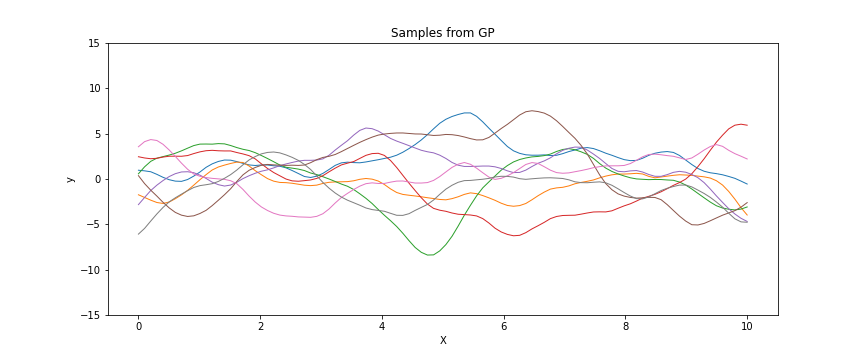
\includegraphics[scale=0.4]{img/05_8/GP_samples.png} % first figure itself
		\caption[GP samples example]{Samples from a GP.}
		\label{fig:GP_samples}
	\end{minipage}\hfill
	\begin{minipage}{0.75\textwidth}
		\centering
		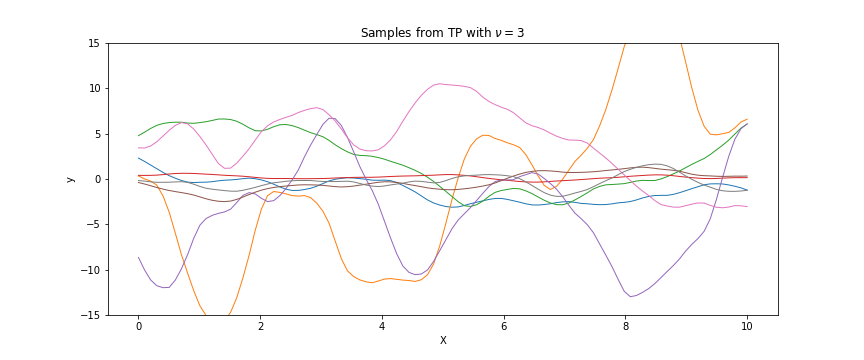
\includegraphics[scale=0.4]{img/05_8/TP_samples.png} % second figure itself
		\caption[TP samples example]{Samples from a TP.}
		\label{fig:TP_samples}
	\end{minipage}
\end{figure}
In figures \ref{fig:GP_samples} and \ref{fig:TP_samples}, the comparison of Gaussian process prior samples (upper) and Student-t (lower) process prior samples are shown. In general the Student-t samples have a broader credibility predictive sample interval compared to the Gaussian process. This leads to a higher tolerance for outliers in the data sets, since the outliers do not impact the covariance as much as with a Gaussian process. A higher parameter $\nu$ leads to a more narrow credibility interval.
After analysing the properties of a Student-t process prior, the conditional distributions can be analyzed. Splitting up a data set into e.g. a test ($\bm{y}_*$) and training ($\bm{y}$) dataset, the respective multivariate Student-t process becomes
\begin{subequations}%multivariate student t conditional distribution
	\label{eq:multivariate student t conditional distribution}
	\begin{align}
	\scriptstyle
	\bm{y}_*|\bm{y} \sim \mathcal{MVT}_{n_*}(\nu+n, K(X_*,X)K(X,X)^{-1}(\bm{y}-\bm{\mu})+\bm{\mu_*},  \nonumber \\
	\scriptstyle
	 \frac{\nu+(\bm{y}-\bm{\mu})^{\top}K(X,X)^{-1}(\bm{y}-\bm{\mu})-2 }{\nu+n-2}(K(X_*,X_*)-K(X_*,X)K(X,X)^{-1}K(X,X_*))) 
	\end{align}
\end{subequations}
with number of datapoints $n_*$ in $\bm{y}_*$ and $n$ in $\bm{y}$ respectively. 
\label{sec:student-t}
\cleardoubleoddpage


\section{Algorithms for stochastic problem computation}
Markov Chain Monte Carlo (MCMC) methods \cite{Geyer_2011} are a class of algorithms that are used to sample a probability distribution that is analytically intractable, or just very complex. A Markov Chain is constructed, that has the same distribution as the target distribution, and recording the chain, the target distribution is uncovered. Since MCMC methods only uncover the true target distribution for very large chain lengths, or even infinite length, a practical convergence criterion is needed to numerically approximate the target multidimensional distributions. We know, that target distributions are calculated via solving integrals of the form \ref{eq:Bayes_with_intractable_term}, so MCMC methods are a likely choice to base further evaluations on. An example of this is depicted in the following figure, where an algorithm is shown that lets the test distribution converge towards the target distribution using the metropolis hastings algorithm.
\begin{figure}[h!]%Metropolis Hastings Convergence Example
	\centering
	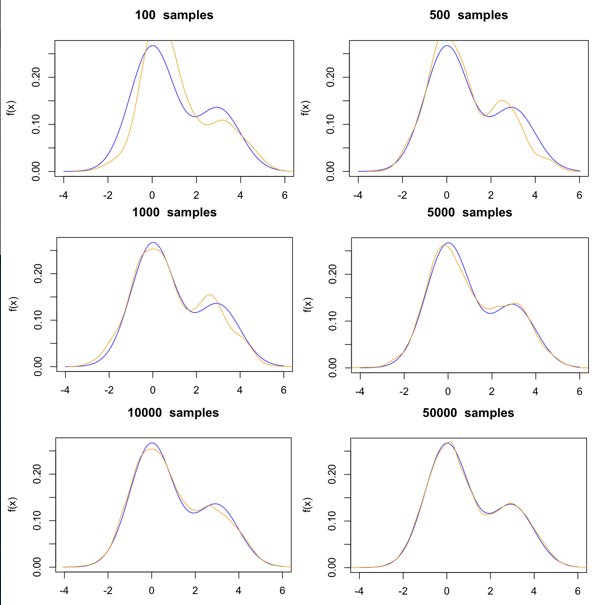
\includegraphics[width=4in]{img/05_6/MetropolisHastingsConvergence.png}
	\caption[Metropolis Hastings Convergence Example]
	{Convergence of the Metropolis Hastings algorithm as an example for Markov chain Monte Carlo methods approximating the target distribution of a bayesian problem. It is clear that more samples lead to a better approximation of the target distribution.}
\end{figure}
A necessary precondition is that the probability density of the target random variable is given up to a constant. If the integral is intractable, MCMC methods can evaluate the integral statistically by generating an ensemble of chains starting at arbitrarily chosen points. A chain is a stochastic process, that moves around randomly on this high dimensional probability surface where moves are generated via Monte Carlo sampling, and then an evaluation of the contribution of this place to the integral is carried out. If the posterior mass is low in some regions, the chain will move away faster from this location, while on the other hand it will spend more moves in regions with higher posterior mass. These Markov chains then have an equilibrium distribution proportional to the target distribution. MCMC methods, even though outperforming generic Monte Carlo algorithms, still suffer from the curse of dimensionality, where regions of higher probability tend to stretch due to a high number of dimensions. Regions with higher probability mass then do not get the proportion of moves necessary in the faster scaling volume of high dimensional space, and contribute less to the solution. This method also implies a problem of when to accept a chain to be converged to a stationary distribution with a reasonable error. Here, the term of rapid mixing becomes important, describing the phenomenon of stationary distributions being reached quickly while starting from arbitrary positions, highlighting the need to sample several chains for non-variational inference algorithms. An extension of the central limit theorem, the Markov chain central limit theorem \cite{Andrieu_2003}, states that for a sequence of random elements forming a Markov chain with the Markov property, the mean of the Markov chain will tend towards a normal distribution. Formally, we have a sequence of random elements $X_1, X_2, X_3, ...$ of some set $\mathcal{X}$ forming the Markov chain with a stationary probability distribution. Also, the initial distribution of the process, the distribution leading to $X_1$ has to be stationary, which entails that $X_1, X_2, X_3, ...$ are identically distributed. Then, the Markov property is necessary, and we need a measurable real-valued function $g$ with $var(g(X_1))<+\infty$.
\begin{subequations}%markov chain central limit theorem prerequisites
	\label{eq:markov chain central limit theorem prerequisites}
	\begin{align}
	\mu = \mathbb{E}(g(X_1)),                                                    \label{eq:mean of initial markov chain step} \\
	\sigma^2 = var(g(X_1)) + 2\sum_{k=1}^{\infty}cov(g(X_1), g(X_{1+k})),         \label{eq:variance markov steps} \\
	\hat{\mu}_n = \frac{1}{n} \sum_{k=1}^{n}g(X_k).                               \label{eq:expected mean markov process}
	\end{align}
\end{subequations}
For $n \to \infty$, we find:
\begin{equation}%markov chain convergence
	\label{eq:markov chain convergence}
	\sqrt{n}(\hat{\mu_n}-\mu) \to \mathcal{N}(0, \sigma^2),         
\end{equation}
resulting in an important feature for convergence. Furthermore, a solution to the curse of dimensionality would be to accept higher autocorrelation and expensive computations by using smaller steps of the chain, which is impractical. More sophisticated methods, like Hamiltonian Monte Carlo reduce autocorrelation while keeping the chain in the desired regions of the probability surface. 

\subsubsection{Hamiltonian Monte Carlo}
Hamiltonian Monte Carlo (HMC) \cite{Duane_1987} is a MCMC method that applies derivatives of the density function to generate efficient transitions when approximating the posterior. The dynamics of the chain is given by Hamiltons equations of motion. The Hamiltonian dynamics simulation is carried out using numerical integration. To achieve this, HMC uses auxiliary momentum variables to form a joint density to draw from. 
\begin{equation}%HMC joint density for regular and auxiliar variables
	p(\rho, \theta) = p(\rho | \theta) p(\theta),
\label{eq: HMC joint density for regular and auxiliar variables}
\end{equation}
where $\rho$ are the auxiliary momentan variables, and $\theta$ are the parameters of the model. By choosing the following distribution for $\rho$, it becomes independent of $\theta$.
\begin{equation}%HMC independent auxiliary variables
	\rho \thicksim \mathcal{N}(0,M).
\label{eq:HMC_independent_auxiliary_variables}
\end{equation}
Here, $M$ is the Euclidian metric, which is just a transformation of parameter space to enhance the efficiency of sampling. The joint density of auxiliary and regular parameters then leads to the combined Hamiltonian
\begin{equation}%HMC Hamiltonian
	H(\rho,\theta) = -log(p(\rho, \theta)) = -log(p(\rho | \theta)) - log(p(\theta)) = T(\rho | \theta) + V(\theta),
\label{eq: HMC Hamiltonian}
\end{equation}
where we define $T(\rho | \theta)$ and $V(\theta)$ as kinetic energy and potential energy respectively, directly analogous to physics. in statistics we find that $T(\rho | \theta) = -log(p(\rho | \theta))$ and $V(\theta) = log(p(\theta))$. The potential energy is often in a statistical context regarded as a log density. From this on, we can use Hamilton´s equations to find find the momentum needed for state transitions. The momentum parameter values are independently drawn using \ref{eq:HMC_independent_auxiliary_variables}, so that momentum is changing across iterations. We use
\begin{subequations}%HMC Hamiltonian equations
	\label{eq:HMC Hamiltonian equations}
	\begin{align}
	\frac{d\theta}{dt} = \frac{\partial H}{\partial \rho} = \frac{\partial T}{\partial \rho},         \label{eq:HMC parameter Hamilton equation} \\
	\frac{d\rho}{dt} = -\frac{\partial H}{\partial \theta} = \frac{\partial T}{\partial \theta} - \frac{\partial V}{\partial \theta} = - \frac{\partial V}{\partial \theta},         \label{eq:HMC auxiliary Hamiltonian equation}
	\end{align}
\end{subequations}
where we have recognized the momentum density $\partial T/\partial \theta$ to be zero, due to the independence of momentum density and target density. This two-state differential equation can then be solved using many integrators. We will discuss the Leapfrog integrator here, since it is most widely used in HMC implementations. In general the Leapfrog integrator uses half integer time steps to calculate velocities and integer time steps to calculate  positions, which pans out to the following updating equations:
\begin{subequations}%HMC Leapfrog update equations
	\label{eq:HMC Leapfrog update equations}
	\begin{align}
	\rho \leftarrow \rho - \frac{\epsilon}{2}\frac{\partial V}{\partial \theta},         \label{eq:LF update rule momentum} \\
	\theta \leftarrow \theta + \epsilon M^{-1}\rho.         \label{eq:LF update rule pamaeters}  
	\end{align}
\end{subequations}
Here, the first update rule is carried out twice, once at the start of a timestep and once at the end. The symplectic Leapfrog integrator has a $\mathcal{O}(\epsilon^3)$ error per step, and globally an error of $\mathcal{O}(\epsilon^2)$. Following a calculated transition, the Metropolis acceptance step begins, where evaluation of the energy of the Hamiltonian leads to accepting the proposed step, or throwing this set of parameters away. The probability of keeping a step can be calculated via
\begin{equation}%Metropolis Acceptance probability of a HMC step
	min(1, exp(H(\rho, \theta))-exp(H(\rho^*, \theta^*))),
\label{eq: Metropolis Acceptance probability of a HMC step.}
\end{equation}
where $\rho^*, \theta^*$ are the proposed values and $\rho, \theta$ the origin of the proposed transition. We do not have to implement HMC by ourself. We can use probabilistic programming languages such as stan. For that, we onl yghave to define the unnormalized posterior density and the approximation thereof is carried out by stan.

\subsubsection{Stochastic Gradient Ascent}
\label{sec:stochastic_gradient_ascent}
Stans variational inference algorithm, Automatic Differentiation Variational Inference \cite{Kucukelbir_2015}, optimizes the ELBO in real-coordinate space. The stochastic gradient ascent obtains unbiased, yet noisy gradients through automatic differentiation and evaluates the ELBO using Monte Carlo integration. Along these gradients, the algorithm ascends using a sequence of adaptive stepsizes. Typically, in practice, the ELBO is sampled with around 100 samples, so that the true ELBO value can be approximated with reasonably high confidence. The ELBO is only evaluated every few iterations, to save computation time, but inside high dimensional manifolds, this seems not to be a problem in practice \cite{stan_manual}. The gradients are also approximated using Monte Carlo Integration, but usually only one sample is drawn, as experience has shown that, while remaining high computational efficiency, stochastic gradient ascent is capable of following such gradients nonetheless. Adaptive step sizes are optimized during a warmup phase where a good value for the single exposed parameter is selected from values spanning multiple orders of magnitude \cite{stan_manual}. This parameter is then used in combination with a finite memory version of adaGrad \cite{Duchi_2011}. In the end, every calculation needs to asses convergence, but since there are no closed form analytical expressions available, the progression of the ELBO values has to be tracked. Using a rolling window, which is heuristically determined, in which the average and median change of the ELBO are computed, we assume convergence if either of those values has fallen below a certain threshold. 
\label{sec:mcmc}
\cleardoubleoddpage

	
	\chapter{Methods}

\section{Mathematical Models}
This work compares different models on metrics of how good a prediction is on the dataset. Different datasets have been used in this evaluation, to compare the results of different models, as well as different subsets of the S\&P500 stocks. The GPLVM, described in section \ref{sec:GPLVM} is the basis for all the models. All explicit kernel functions will be provided with the example of a squared exponential kernel.

\subsection{Gaussian Process Latent Variable Model in Finance}
\ref{sec:gplvm_finance}
The GPLVM, as explained earlier in section \ref{sec:GPLVM}, considers the same variance for each stock and also the same noise variance. Stocks, however, have different volatilities, which in turn are displayed in the model as variances. Therefore, we reparametrize the model. Given the data matrix $Y = (\bm{y}_1, ..., \bm{y}_N)^{\top} \in \mathbb{R}^{N \times D}$ and the latent spaces $X = (\bm{x}_1, ..., \bm{x}_N)^{\top} \in \mathbb{R}^{N \times Q}$, the model becomes 
\begin{equation}%eq:financial_model_gplvm
	Y_n \thicksim \mathcal{N}(0,K),
	\label{eq:financial_model_gplvm}
\end{equation}
where the mean is assumed to be $0$, and the covariance matrix to be given by $K$. The covariance matrix is constructed using the $X$s, the time dependent correlation matrix $K_{\text{corr}}(t)$, noise variances $\sigma_i$ and the variance matrix $\Sigma = \text{diag}(\sigma_i)$. 
\begin{equation}%eq:constructed_cov_matrix
	K = \Sigma K_{corr}(d) \Sigma + \sigma_k \mathbb{1}
	\label{eq:constructed_cov_matrix}
\end{equation}
An entry of the resulting covariance matrix $K$ looks like
\begin{equation}%eq:GPLVM_Kx_entry
	k(d_i,d_j) = \alpha^2 exp\Big[-\frac{1}{2l^2}(d_i-d_j)\Big]+ \delta_{ij}(\sigma^2 + g),
	\label{eq:GPLVM_Kx_entry}
\end{equation}
where $k(d_i,d_j)$ is the covariance function, $\alpha$ and $l$ are the kernel hyperparameters, $\sigma$ is the variance and $g$ is a very small value (jitter) added to the diagonal of the matrix, to prohibit singular covariance matrices and thus ensure invertibility. This describes a nonlinear mapping from latent space positions to data space, 
\begin{equation}%eq:nonlinear_map
	Y_{:,d} = f_d(X_{:,d}) + \epsilon_{:,d}.
	\label{eq:nonlinear_map}
\end{equation}
Here, the function $f_d$, that is the map, is a $\mathcal{GP}(0,k)$, with a nonlinear kernel function $k$. The noise term is $\epsilon_{:,d} \thicksim \mathcal{N}(0,\text{diag}(\bm{\sigma_{n}}^2))$, which directly leads us towards accepting different volatilities for different stocks. We can then decompose the covariance Matrix $K$ into a correlation matrix and diagonal noise matrices. 
\begin{equation}%eq:covariance_decomposition
	K = \Sigma K_{\text{corr}} \Sigma,
	\label{eq:covariance_decomposition}
\end{equation}
which, for a stationary kernel becomes
\begin{equation}%eq:stationary_decomposition
	K_{\text{stationary}} = \Sigma k_{\text{stationary}}(X,X) \Sigma + k_{\text{noise}}(X,X)
	\label{eq:stationary_decomposition}
\end{equation}
and the likelihood of the full model is given by
\begin{equation}%eq:gplvm_likelihood
	p(Y|B,\bm{\theta}) = \prod_{d=1}^{D} \mathcal{N}(Y_{:,d}|\bm{0}, K) = \frac{1}{(2\pi)^{0.5 \cdot ND} K^{0.5 \cdot D}} \exp(-0.5\text{tr}(K^{-1}YY^{\top}))
	\label{eq:gplvm_likelihood}
\end{equation}
The generative process for this model then becomes
\begin{subequations}%eq:generative_process_gplvm_finance
	\label{eq:generative_process_gplvm_finance}
	\begin{align}
		l \thicksim \text{Inv-Gamma}(3,1),         \nonumber \\
		\alpha \thicksim \text{Inv-Gamma}(3,1),         \nonumber \\
		\sigma_n \thicksim \mathcal{N}(0,0.5),         \nonumber \\
		\sigma_k \thicksim \mathcal{N}(0,0.5),         \nonumber \\
		X[n] \thicksim \mathcal{N}(0,1),         \nonumber \\
		Y[d] \thicksim \mathcal{N}(0,K).          \\
	\end{align}
\end{subequations}


\subsection{Time Dynamic Gaussian Process Latent Variable Model}
\label{sec:td_gplvm}
The Time Dynamic Gaussian Process Latent Variable Model (TD-GPLVM) allows the latent space positions to vary over time. Instead of describing $Y \in \mathbb{R}^{N \times D}$ and $X \in \mathbb{R}^{N \times Q}$, which is fixed in latent space, we increase the dimension of $X$ to $X \in \mathbb{R}^{N \times Q \times D}$, where $X_d \in \mathbb{R}^{N \times Q}$ and $X_{n,q,:} \in \mathbb{R}^{D}$. $X_{n,q,:}$ then follows a Gaussian Process.  
\begin{equation}%TD-GPLVM Latent Space
	 X_{n,q,:}  \sim \mathcal{N}(0, K_{DD})
\label{eq: TD-GPLVM Latent Space}
\end{equation}
The computational complexity of this process is of order $\mathcal{O}(D^3)$, because of the inversion of $K_{DD} \in \mathbb{R}^{D \times D}$. Therefore, only a few days of observations can be modelled simultaneously.  
The idea of this model is to incorporate a time dependent correlation of latent variables, which may exist for certain datasets. In matrix notation, the covariance matrices are formed through the quadratic diagonal form of the time dependent correlation matrix $K_{corr}(t)$, noise variance $\sigma_n$ and variance matrix $\Sigma = \text{diag}(\sigma_i)$.
\begin{equation}%TD-GPLVM matrix form
	K = \Sigma K_{corr}(d) \Sigma + \sigma_n \mathbb{1}
\label{eq: TD-GPLVM matrix form}
\end{equation}
An entry of the resulting covariance matrix $K_x$ looks like
\begin{equation}%TD-GPLVM K_x entry
	K_{ij}=k(x_i,x_j) = \alpha_i\alpha_j exp\Big[-\frac{1}{2l^2}(d_i-d_j)\Big]+ \delta_{ij}(\sigma_i^2 + g),
\label{eq: TD-GPLVM K_x entry}
\end{equation}
where $k(x_i,x_j)$ is the covariance function, $\alpha_i\alpha_j$ and $l$ are the kernel hyperparameters, $\sigma_i$ are the variances and $g$ is a very small value (jitter) added to the diagonal of the matrix, to prohibit singular covariance matrices and thus ensure invertibility. The inputs to the covariance function are $d_i$ and $d_j$, the $i$th or $j$th entry of a vector containing ordered timesteps $\bm{d} = (d_1, d_2, d_3, ... , d_D)^{\top}$. The covariance function of $K_y$ then becomes
\begin{equation}%TD-GPLVM K_y entry
	k_y(x_i[d], x_j[d]) = \alpha_i\alpha_j exp\Big[-\frac{1}{2l_y^2} (x_i[d]-x_j[d])\Big] + \delta_{ij}(\sigma_i^2 + g)
\label{eq: TD-GPLVM K_y entry}
\end{equation}
where again, $k_y(x_i[d], x_j[d])$ is the kernel function, $\alpha_i\alpha_j$ and $l_y^2$ are the kernel hyperparameters, and $\sigma_y$ is the variance. Also, $g$ continues to be a very small value added as jitter to the diagonal of the covariance matrix to prevent singularity and $x_{i}[d]$ and $x_{j}[d]$ are the positions of asset $i$ and $j$ at time point $d$ in latent space $\mathcal{X}$. After conditioning the model was parametrised by
\begin{subequations}
	\label{eq:TD-GPLVM conditioning}
	\begin{align}
	l \sim \text{gamma}(10,5)         \nonumber \\
	l_y \sim \text{inv-gamma}(3,1)         \nonumber \\
	\sigma_k \sim \mathcal{N}(0, 0.5) \nonumber \\
	\sigma_n \sim \mathcal{N}(0, 0.05) \nonumber \\
	X[n,q,:] \sim \mathcal{N}(\bm{0}, K_x) \nonumber \\
	Y[:,d] \sim \mathcal{N}(\bm{0}, K_y[d]) \nonumber
	\end{align}
\end{subequations}
the stan code can be found in Appendix \ref{sec:model_code}, as \textit{gplvm-time.stan}.

\subsection{Volatility Gaussian Process Latent Variable Model}
\label{sec:v_gplvm}
Another model that may solve problems of simpler models is the Volatility Gaussian Process Latent Variable Model (V-GPLVM). The V-GPLVM works similar to the regular GPLVM, but the diagonal matrix with the variances, which work as a placeholder for the proportional volatility, is time dependent. 
\begin{equation}%V-GPLVM matrix form
	K_d = \text{diag}\Big(\Sigma(:,d)\Big) K_{corr} \text{ diag}\Big(\Sigma(:,d)\Big) + \text{diag}(\sigma_i)
\label{eq: V-GPLVM matrix form}
\end{equation}
Again, $\sigma_n$ are the noise variances, and $K_{corr}$ is the correlation matrix. $\text{diag}(\Sigma(:,d))$ is the time dependent diagonal variance matrix, which will be inferred throughout the process. While evaluating the programm, these matrices are constructed from columns of the total variance matrix $\Sigma \in \mathbb{R}^{N\times D}$, representing the inferred values for variances for stocks on a given time step. The latent space Gaussian Process prior is just a standard normal distribution $\mathcal{N}(0,1)$, while the Gaussian Process over the data space if more complex. 
\begin{equation}%V-GPLVM K_y Element
	K[d]_{ij} = \Sigma[d,i] \Sigma[d,j] \Bigg( exp\Big(-\frac{1}{2l^2}(x_i-x_j)\Big)\Bigg)+ \delta_{ij}(\sigma_k^2 + g)
\label{eq: V-GPLVM K_y Element}
\end{equation}
After conditioning the model priors were parametrised like
\begin{subequations}
	\label{eq:V-GPLVM conditioning}
	\begin{align}
	X[n] \sim \mathcal{N}(0,1)                  \nonumber \\
	\log\Sigma[d] \sim \mathcal{N}(0,1)         \nonumber \\
	\sigma_k \sim \mathcal{N}(0,1)              \nonumber \\
	l \sim \text{inv-gamma}(3,1)                \nonumber \\
	Y[:,d] \sim \mathcal{N}(\bm{0}, K[d]), \nonumber
	\end{align}
\end{subequations}
where $K$ is evaluated after Cholesky factorising the kernel matrix slices $K[d] \in \mathbb{R}^{N\times Q}$ through Cholesky decomposition $K = LL^*$, where the matrix is decomposed into a lower triangular matrix $L$. Using the Cholesky Decomposition reduces computing time, while maintaining numerical stability. The method is more stable and cost efficient for matrix inversion, which, as previously discussed, is the major bottleneck for computing time, since using the decomposition reduces the needed number of evaluations to half. The stan code can be found in Appendix \ref{sec:model_code} as \textit{gplvm-vola.stan}.
\label{sec:models}
\cleardoubleoddpage

\section{Programs}
\subsection{Programm Sequence}
\begin{figure}%fig:program_sequence
	\label{fig:program_sequence}
	\centering
	\includegraphics[width=60mm]{img/06_1/ThesisOverview.png}
	\caption[Overview of the program sequence.]
	{Program Sequence overview according to DIN 66001 \cite{DIN66001}.}
\end{figure}
As shown in the program sequence overview \ref{fig:program_sequence}, the process executed starts with a second programm, decoupled from the acutal calculations, downloading stock market data from yahoo finance \cite{yahoo_finance} with previously specified tickers from the S\&P500 index over an also specified time period, where the full time period is 2010/01/01-2013/01/01. In the calculation sequence a dataset is downloaded, and lists of values for latent dimensions (Qs), kernel functions (kernels), and different models are specified. With these, the models written in stan are compiled by the stan model compile function, and saved as a pickled model. This model is then executed for all combinations of Qs and kernels using the variational bayes algorithm. Variational Bayes outputs diagnostic information of the model, and samples for all parameters specified in either the parameter block or the generated quantities block of the stan model. These are both saved as files for later checking of the models diagnostic, through both the diagnostic information, most notably ELBO values from the variational inference, and the samples, from which e.g. $R^2$ values can be calculated. With this, different sanity checks are applied, like plotting the true measured values against the predictions calculated from the models learned structure, checking the values from different sampled variables agains the expectations. All of these will be discussed in detail in the results section \ref{sec:results}. 

\subsection{The stan language}
The stan language was referenced a few times before, in this section a little more light will be shed on how to apply it. To recap, stan \cite{stan_overview} is a program that compiles an efficient \textit{c++} program from a textfile in which in the stan language a statistical model is specified. This text file is comprised of up to 9 blocks, in which different parts of the model are specified and whose compiled program parts are executed at different times during the execution of the compiled program. This will be henceforth referenced to as "evaluation of a block". At first, the data block is evaluated. It specifies the variables that are fixed, and are handed to the compiled program for execution. Typical entries are a number of which kernel function to use, the data matrix $Y$, as well as some initially fixed variables like a jitter or the number of dimensions of the latent space $Q$. This block can be preceded by a functions block, which is not needed for execution, but can be convenient when the model has some parts of code that need to be executed several times. After the data block, a block called transformed data can be introduced, in which constants and transforms of the content of the data block can be specified. This can be used to e.g. create null-vectors, which in a lot of models are used as starting parameters of a mean. Then follows the parameters block, which is filled with variables that are to be inferred, reckoning sampled or optimized, during the execution of the program. mPosterior distributions of variables specified as parameters of the model in the parameters block are approximated during variational inference. The parameters can be transformed in the transformed parameters block. No statements are allowed in the previous blocks, except for transformed data and transformed parameters block. In the model block, the log of the unnormalized posterior density is specified, and the sampling statements of parameters are selected. Finally, the generated quantities block allows for the creation of derived variables, containing the variables from the parameters block. \newline \newline
Formally, all blocks are optional, but a typical sensible program will have at least a data block, parameters, and a model block. This ordering of the blocks is necessary, and disobeying it will break the program. In the following listing, a simple Gaussian process is depicted \cite{stan_manual}.
\lstset{basicstyle=\tiny, style=Stan}
\begin{lstlisting}
	data {
		int<lower=1> N;
		real x[N];
	}
	transformed data {
		matrix[N, N] K = cov_exp_quad(x, 1.0, 1.0);
		vector[N] mu = rep_vector(0, N);
		for (n in 1:N)
		K[n, n] = K[n, n] + 0.1;
	}
	parameters {
		vector[N] y;
	}
	model {
		y ~ multi_normal(mu, K);
	}
\end{lstlisting}
Variables declared in a program block will have scope over all blocks, in a way be global, and functions may be used in all appropriate blocks. Exceptions to this rule are, that variables from the model block are local, and variables declared in a later block are not yet known to an earlier block. Functions that generate random numbers are limited to the transformed data and generated quantities block, and functions that modify log probability may only be used in the transfomred parameters and model block. This stan language, with a syntax close to that of other high-level programming languages like \textit{python} or \textit{c++}, is comparably easy to write and learn, while compiling very efficient programs. Writing down the model in mathematical terms almost directly translates to the stan model, which makes application of stan very practical, especially for users without intensive training in computer science \cite{stan_manual}. A compiled stan model can be used different ways. One can optimize the defined log posterior density, approximate their posterior using variational inference or sample from the posterior using Hamiltonian Monte Carlo. In the following figure, a more complex model is shown, which is referred to as GPLVM throughout this work.
\lstset{basicstyle=\tiny, style=Stan}
\begin{lstlisting}
functions {
	matrix cov_linear(vector[] X1, vector[] X2, real sigma){
		int N = size(X1);
		int M = size(X2);
		int Q = num_elements(X1[1]);
		matrix[N,M] K;
		{
			matrix[N,Q] x1;
			matrix[M,Q] x2;
			for (n in 1:N)
				x1[n,] = X1[n]';
			for (m in 1:M)
				x2[m,] = X2[m]';
			K = x1*x2';
		}
		return square(sigma)*K;
	}
	
	matrix cov_matern32(vector[] X1, vector[] X2, real sigma, real l, real jitter){
		int N = size(X1);
		int M = size(X2);
		matrix[N,M] K;
		real dist;
		for (n in 1:N)
			for (m in 1:M){
				dist = sqrt(squared_distance(X1[n], X2[m]) + jitter);
				K[n,m] = square(sigma)*(1+sqrt(3)*dist/l)*exp(-sqrt(3)*dist/l);
		}
		return K;
	}
		
	matrix cov_matern52(vector[] X1, vector[] X2, real sigma, real l, real jitter){
		int N = size(X1);
		int M = size(X2);
		matrix[N,M] K;
		real dist;
		for (n in 1:N)
			for (m in 1:N){
				dist = sqrt(squared_distance(X1[n], X2[m]) + jitter);
				K[n,m] = square(sigma)*(1+sqrt(5)*dist/l+5*square(dist)/(3*square(l)))*exp(-sqrt(5)*dist/l);
		}
		return K;
	}
	
	matrix cov_exp_l2(vector[] X1, vector[] X2, real sigma, real l, real jitter){
		int N = size(X1);
		int M = size(X2);
		matrix[N,M] K;
		real dist;
		for (n in 1:N)
			for (m in 1:M){
				dist = sqrt(squared_distance(X1[n], X2[m]) + jitter);
				K[n,m] = square(sigma) * exp(-0.5/l * dist);
		}
		return K;
	}
	
	matrix cov_exp(vector[] X1, vector[] X2, real sigma, real l, real jitter){
		int N = size(X1);
		int M = size(X2);
		matrix[N,M] K;
		real dist;
		int Q = rows(X1[1]);
		for (n in 1:N)
			for (m in 1:M){
				dist = 0;  
				for (i in 1:Q)
					dist = dist + fabs(X1[n,i] - X2[m,i]);
					K[n,m] = square(sigma) * exp(-0.5/l * dist);
		}
		return K;
	}
	
	matrix kernel_f(vector[] X1, vector[] X2, real sigma, real l, 
	real a, int kernel, vector diag_stds, real jitter){
		int N = size(X1);
		int M = size(X2);
		matrix[N,M] K;
		if (kernel==1)
		K = cov_linear(X1, X2, a);
		else if (kernel==2){
			K = cov_exp_quad(X1, X2, sigma, l);
			for (n in 1:N)
			K[n,n] = K[n,n] + jitter;
			K = quad_form_diag(K, diag_stds);
		}
		else if (kernel==3){
			K = cov_exp(X1, X2, sigma, l, jitter);
			K = quad_form_diag(K, diag_stds);
		}
		else if (kernel==4){
			K = cov_matern32(X1, X2, sigma, l, jitter);
			K = quad_form_diag(K, diag_stds);
		}
		else if (kernel==5){
			K = cov_matern52(X1, X2, sigma, l, jitter);
			K = quad_form_diag(K, diag_stds);
		}
		return K;
	}
}
data {
	int<lower=1> N;
	int<lower=1> D;
	int<lower=1> Q;
	matrix[N,D] Y;
	int<lower=1,upper=5> kernel;
	real<lower=0> jitter;
}
transformed data {
	vector[N] mu = rep_vector(0, N);
}
parameters {
	vector[Q] X[N];                       
	real<lower=0> kernel_lengthscale;     
	vector<lower=0>[N] diag_stds;        
	vector<lower=0>[N] noise_std;          	
	real<lower=0> alpha;                  
}
transformed parameters {
	matrix[N,N] L;
	real R2 = 0;
	{
		matrix[N,N] K = kernel_f(X, X, 1., kernel_lengthscale, 
		alpha, kernel, diag_stds, jitter);
		
		for (n in 1:N)
		K[n,n] = K[n,n] + pow(noise_std[n], 2) + jitter;
		L = cholesky_decompose(K);
		
		R2 = sum(1 - square(noise_std) ./diagonal(K) )/N;
	}
}
model {
	for (n in 1:N)
	X[n] ~ normal(0, 1);
	
	diag_stds ~ normal(0, .5);
	noise_std ~ normal(0, .5);
	kernel_lengthscale ~ inv_gamma(3.0,1.0);
	alpha ~ inv_gamma(3.0, 1.0);             
	
	for (d in 1:D) 
	col(Y,d) ~ multi_normal_cholesky(mu, L);
}
generated quantities {
	matrix[N,N] K = kernel_f(X, X, 1., kernel_lengthscale, 
	alpha, kernel, diag_stds, jitter);
}
\end{lstlisting}

\subsection{Conditioning}
Stan´s algorithms approximate the density, or penalized maximum likelihood, step-, and gradient based. This leads to the statistical efficiency of the stan programs relying on posterior curvature, which is not captured by these algorithms. To solve this problem, one has first to look at the Hessian, which is defined in a statistical context by
\begin{equation}%Hessian Conditioning
	H(\theta) = \nabla \nabla log (p(\theta | y))
\label{eq: Conditioning with Hessian principle}
\end{equation}
where again, $\theta$ is the parameter vector, and y is the data. Here, the Hessian is a second order approximation to curvature, which can be expressed in matrix form as
\begin{equation}%Hessian Conditioning Matrix Form
	H_{i,j}(\theta) = \frac{\partial^2 log (p(\theta | y))}{\partial \theta_i \partial \theta_j}.
\label{eq: Conditioning with Hessian Matrix}
\end{equation}
Using this, we find that comparing the largest and smallest eigenvalue of $H$ as a ratio gives a good estimation of how much of a problem the aforementioned curvature presents. That ratio represents the largest and smallest curvature values, where typically the step size of a gradient based algorithm is bounded by the highest curvature value. Optimizing this highest curvature leads to better conditioning of the model, which in turn enhances computation cost and time. In all models, except the most simple ones (e.g. multivariate normal distributions), the Hessian will vary as the set of parameters $\theta$ varies. And for the assumption of fixed adaptation parameters, which is true in all algorithms except Riemannian Hamiltonian Monte Carlo, which in turn is not implemented in stan and computationally very expensive, a high variance of curvature will lead to worse adaptations covering the entire density sufficiently. Variable transformations are often proposed with the aim of improving the conditioning of the Hessian. This usually entails, or is transferable with making the Hessian more consistent across relevant parts of the density. For variational inference the iterative algorithm then finds a single point as curvature of the path from the initial values of the parameters to the solution. Taking this into account, another way of improving statistical efficiency is reparameterising the model in such a fashion, that the same results may be calculated, using a better conditioned density or maximum likelihood. Diving into this would entail redefining bayesian posteriors as to what they technically are, probability measures, so this is left for further work. 
\label{sec:programs}
\cleardoubleoddpage
	
	\chapter{Results}

\section{GPLVM}
%Notes:   
%Reason for assumption that mean of this distribution is the most likely the correct value, due to nature of the distributions. 
%scalar samples from vb is symmetrically weighted to both sides? interpretation?
%Possible influences on this deviation from the expected predictions: 
% absolute return value (higher returns get underestimated, lower returns get overestimated, leads to models with incorporated volatility, or broader flanks), 
% input data size (possible masking of data structure through sheer size, size prop. complexity of data structure in regime of N >= x1(???), possible data sizes not reflecting all structure due to missing inputs N<=x1, find optimum.), 
% choice of data (randomized stocks, structured stocks by ressort, structured stocks by alphabet in company name list) and observed pros and cons of these choices, 
% number of observed days for training (influence of training days and influence of how the progression of time influences prediction accuracy), 
% influence of hyperparameters (kernel lengthscale prop. to flexibility of change in single function draws from function space, function noise as prop. to self correlation since only added to diagonal, influence of jitter for numerical stability, influence of kernel noise prop. to e.g. volatility as it is unique to every stock (even though it is observed only during once)), 
% influence of latent positions/correlations (how does the grouping change with N-size, D-size) and 
% sampler ELBO convergence (should the convergence ratio be chosen smaller to definitely land in a minimum, should sampler do more runs because differences between found minima is large, etc.). 
% PLOTS Percentage of overpredicted and underpredicted stocks (in dependence of N-size, stock-groups, effect of stock groups rising and falling together (source???)). Influences of kernels, Qs. 

The Gaussian process latent variable model (GPLVM) is the basis of all following models. This stochastic process tries to learn a covariance structure from the data. All stocks are assigned a position in latent space, which influences the covariance structure the process can reproduce. This influences the covariance matrix, which is the key element of the learning equation of the GPLVM, representing the covariance structure learned. Data is fed into the model as a matrix of size $\mathbb{R}^{NxD}$, with $N$ stocks' returns observed over a timespan of $D$ days. If no data was available, the spot in the matrix was assumed to be 0, which is a reasonable assumption, since returns over small timespans are close to zero with only a small drift towards positive values. Then, the calculation specified by the model, as explained in more detail in the previous chapter \ref{sec:models}, is carried out. Samples from the Variational Bayes algorithm are generated and used to calculate the mean prediction for a specific entry of a matrix, vector, or simply a scalar. With these, the interpretation is carried out. 
\begin{figure}[h!]%cov_entries_gplvm
	\centering
	\begin{subfigure}[b]{0.4\textwidth}
		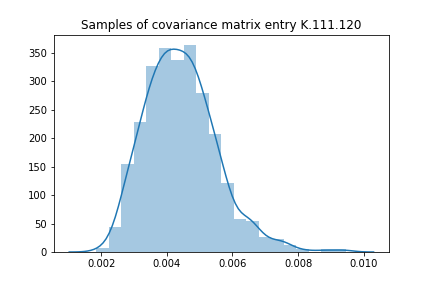
\includegraphics[width=\textwidth]{img/07_0/K_111_120_samples.png}
		\caption{The entry 111/120 of the covariance matrix of the GPLVM model trained on a dataset of $N=120$, $D=754$. For this covariance entry, the algorithm has converged sufficiently and sufficiently fast.}
		\label{fig:K_111_120_gplvm}
	\end{subfigure}
	\begin{subfigure}[b]{0.4\textwidth}
		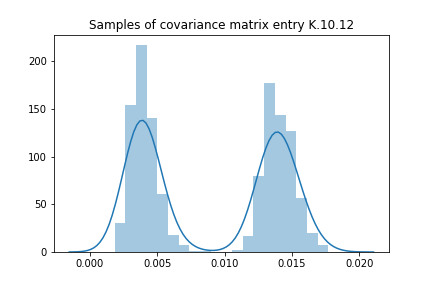
\includegraphics[width=\textwidth]{img/07_0/K_10_12_samples.png}
		\caption{The entry 10/12 of the covariance matrix of the GPLVM model trained on a dataset of $N=120$, $D=754$. For this covariance entry, the algorithm has not converged sufficiently or sufficiently fast.}
		\label{fig:K_10_12_gplvm}
	\end{subfigure}
	\caption{}
	\label{fig:cov_entries_gplvm}
\end{figure}
The plots in \ref{fig:cov_entries_gplvm} show the distribution sampled by the variational inference algorithm as kde and histogram plot of two entries of the covariance matrix. The ratio of sampled values in the main peak compared to the other peaks, as well as the position of the global maximum of this distribution compared to the effectively used value, which is the overall mean and further on used quantity, give a good estimate of the error that is effecting the further results for a calculation where the ELBO has converged. Entry K.10.12, figure \ref{fig:K_10_12_gplvm}, shows critical behavior where the algorithm probably has not converged sufficiently, or where different values seem to provide stable solutions. This is especially interesting, since time-dependent solutions to the covariance between two stocks seem like a viable alternative. The entry K.111.120, figure \ref{fig:K_111_120_gplvm} instead provides a clearer image of what was expected, where the mean is closer to the maximum of probability mass. The learning equation,
\begin{equation}%GPLVM Learning Equation
	\hat{Y}_{GPLVM} = K [(K+\delta_{ij}\sigma_{n})Y],
	\label{eq:GPLVM_learning_equation}
\end{equation}
is used to calculate predictions from the model. Testing the prediction power of models is usually done in several steps, where the first step is to test it against predicting the initial data. With the predictions, we can calculate errors based on the model reproducing the dataset it was trained on, resulting in $\hat{Y}$, a matrix of equal size as $Y$. Since the model includes uncertainty and noise, we do not expect a perfect reconstruction of the data fed into the model. Comparing the data with the predictions yields interesting insight, since several possible errors can be directly visible from these results. But first, it is necessary to discuss various ways of quantifying the quality of a model. The Evidence Lower Bound, which was introduced in chapter \ref{sec:bayes}, is a unit-less measure of the quality of a model. The higher the ELBO, the better the results. Comparing the ELBO values gives insight into how good a model was able to reproduce the true posterior with the variational inference distribution approximation of the true posterior, using KL-Divergence. The initial expectation is that models with more dimensions taken into account in the latent space (higher values of Q) perform better, and how more sophisticated kernels outperform less sophisticated kernels like the linear kernel \cite{Nirwan_2019}. As another measure of performance, the $R^2$ values of the models are calculated and plotted in the same fashion as the ELBO values. These are calculated of the data and predictions using the \textit{LinearRegression} model from \textit{arviz} \cite{arviz_2019}, which uses the regular definition of the coefficient of determination ($R^2$). 
\begin{equation}%Coefficient of Determination R^2
	R^2 = 1 - \frac{\sum (Y-\hat{Y})^2}{\sum (Y-\bar{Y})^2}
	\label{eq: GPLVM R^2 calculation}
\end{equation}
The coefficient of determination is a measure of how well the model has reconstructed the predictions as a function of the data, but it still has missing information. If we plot the data points against the corresponding predictions, we would expect a single straight line with slope 1 and intercept 0 for a perfect result. Since the model incorporates noise, we still would expect the model to have a slight deviation from this line, but it should be centered around the line. If the deviation is centered around the line, a Huber regression fit through the data-prediction pairs would also have a slope of 1 and an intercept of 0.  Huber regression was chosen over linear regression, due to the outliers in predictions only accounting linearly instead of quadratic when doing linear least squares optimization during regression, and therefore provided much more stable and reliable information about the intercept and slope values. For more information, see Appendix \ref{sec:huber_reg}. While reconstructing the model initially tested against these kind of data in \cite{Nirwan_2019}, the plots showed an abnormality.
\begin{figure}%CENTRAL IMAGE with problem statement of Y-Y_hat pairs reflecting problem.
	\centering
	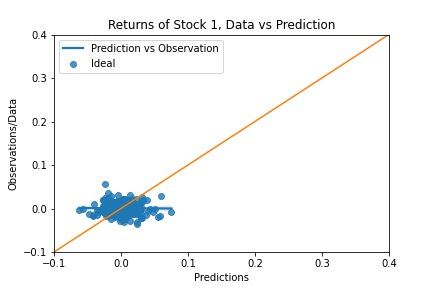
\includegraphics[width=4in]{img/07_0/problem.jpg}
	\caption[Data-Prediction Plot GPLVM]
	{An example of a Y-$\hat{Y}$-pair plot of a stock fit with a Stochastic Process Latent Variable Model. A linear least squares fit is added, highlighting the observed effect of the predictions not accurately reflecting the data. Predictions on a regular basis seem to underestimate comparably high returns, and overestimate comparably low returns, resulting in a slope of the linear fit that is way off of the expectation.}
	\label{fig:gplvm_pair_plot_central}
\end{figure}
The model at hand overestimates lower returns, and underestimate higher returns, resulting in non-optimal ELBO and $R^2$ values. Higher ELBO values represent better estimation of the true posterior, but are not able to be interpreted with a higher bound due to the nature of the KL-divergence. $R^2$ values, the coefficients of determination, are a measure of the prediction quality, as a numerical value of how similar data and predictions are. A value relatively close to one is optimal, but due to the nature of how noisy stock market data is, a value of 1 would not be desirable. Because then the model would have learned a lot of noise as feature. Models that show considerably lower values in ELBO compared to the respective other models sharing characteristics probably have not converged towards the optimal point on the energy landscape, for example $Q=3$ and $Q=6$ with the exponential kernel in figure \ref{fig:gplvm_ELBO_R2}. 
\begin{figure}
	\centering
	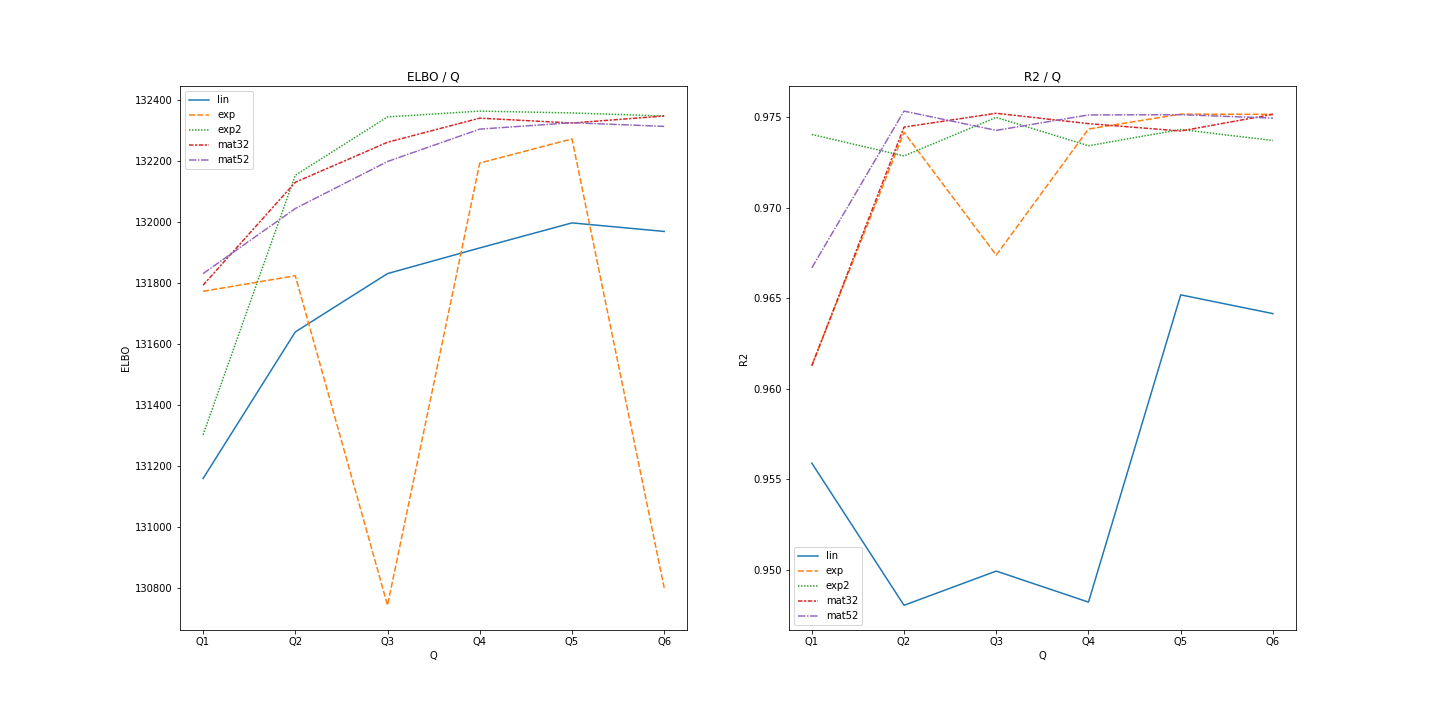
\includegraphics[width=7in]{img/07_0/modelGPLVM_Qs.png}
	\caption[ELBO and $R^2$ comparison for the GPLVM model]{ELBO and $R^2$ values for the GPLVM model and $N=60$, $D=754$. }
	\label{fig:gplvm_ELBO_R2}
\end{figure}
We can find another metric of model quality in the distribution and mean values of intercepts, as well as slope values. These distributions show how the model has predicted the slopes, figure \ref{fig:gplvm_slopes}, and intercepts, figure \ref{fig:gplvm_intercepts}, of all stocks entailed in the data matrix. Experiments show good agreement with expectations for the slopes, since they are close to the expected value of 1. Still they remain mostly to the left side of the bar at slope$=1$, coinciding with the expectation that a model can never learn everything about a naturally noisy system. The distributions of the intercepts should be centered around the vertical line at intercept$=0$, which would imply that almost the same number of stocks are over predicted as are under predicted.
\begin{figure}%Intercept distributions
	\centering
	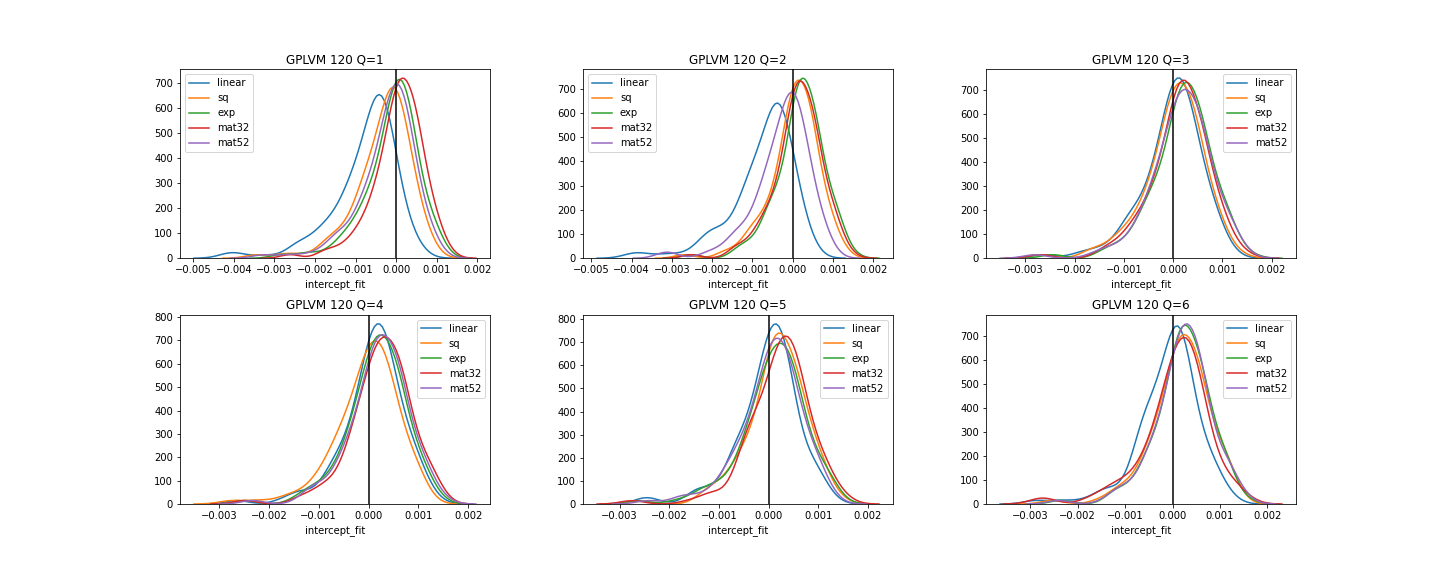
\includegraphics[width=7in]{img/07_0/intercept_fit_gplvm_120.png}
	\caption[Intercept Distributions for GPLVM]{Comparing the distributions of stock slope values from the GPLVM model with different kernel functions over the scope of all latent dimensions. }
	\label{fig:gplvm_intercepts}
\end{figure}
\begin{figure}%Slope distributions
	\centering
	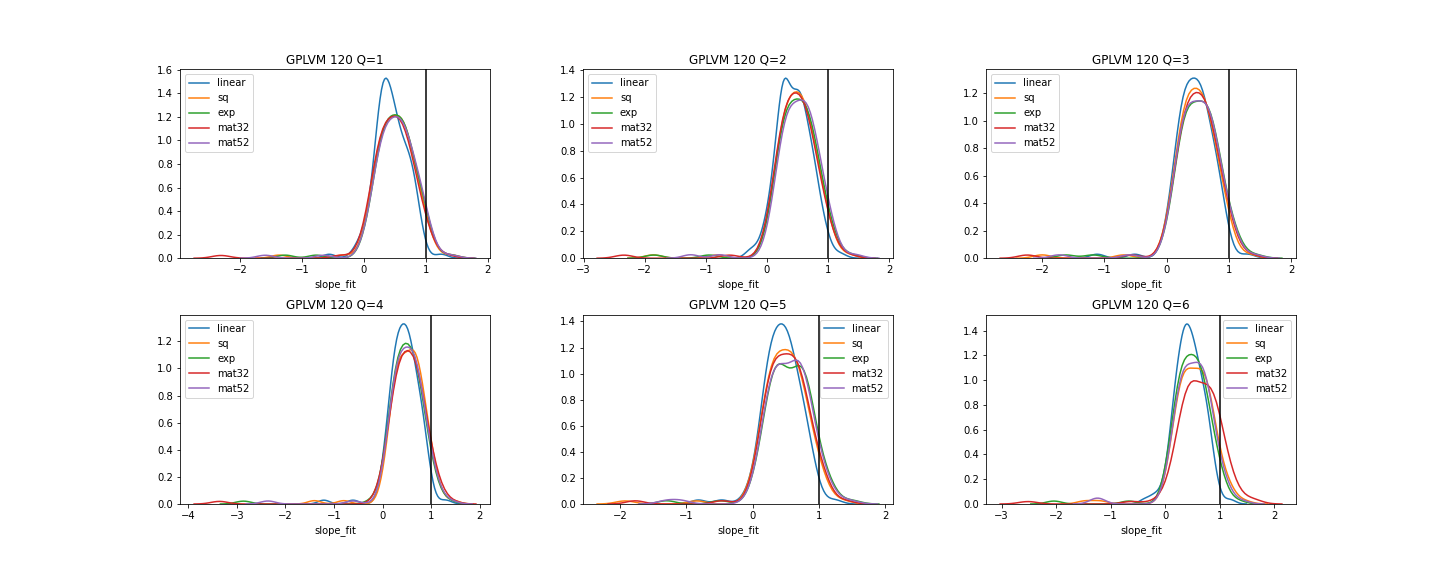
\includegraphics[width=7in]{img/07_0/slope_fit_gplvm_120.png}
	\caption[Slope distributions for GPLVM]
	{Comparing the intercept values of the GPLVM model with different kernel functions over the scope of all latent dimensions. }
	\label{fig:gplvm_slopes}
\end{figure}
\newline \newline
Several sanity checks for the model are displayed, where the distributions of the samples, or just the distributions of the values of the entries of the vector-like or matrix-like objects are plotted. Within these checks, larger samples of outliers can be detected, that may stem from local minima in the energy landscape in the variational inference solver. 
\begin{figure}%fig:gplvm_noises   Observation noise distribution sanity checks
	\centering
	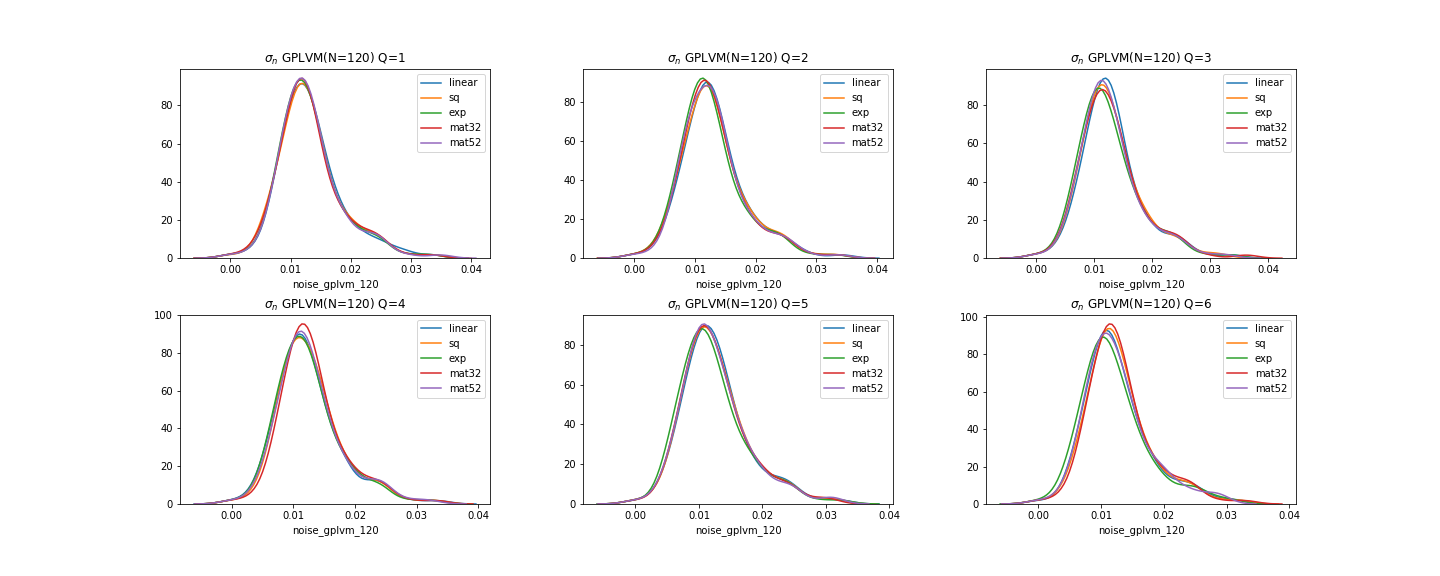
\includegraphics[width=7in]{img/07_0/noise_GPLVM_120.png}
	\caption[Signal Noise distributions GPLVM]
	{Distributions of vector elements of $\sigma_n$. The closer values are to 0, the more accurate the measurements are according to the model. The observation noise is non-isotropic.}
	\label{fig:gplvm_noises}
\end{figure}
Figure \ref{fig:gplvm_noises}, together with the learning equation, gives a direct interpretation of the kernel noise as the observation noise, since it is added to the diagonal of the covariance matrix. These entries resemble the self-correlation of the stocks. Also, it is necessary to point out, that these kernel density estimate plots of the variables can be misleading, since e.g. the noise is restricted to $\mathbb{R}_0^+$, since noise can not improve the measurement accuracy to be better than perfect.
\begin{figure}%fig:gplvm_variances     Variance noise distribution sanity checks ~ volatility per stock
	\centering
	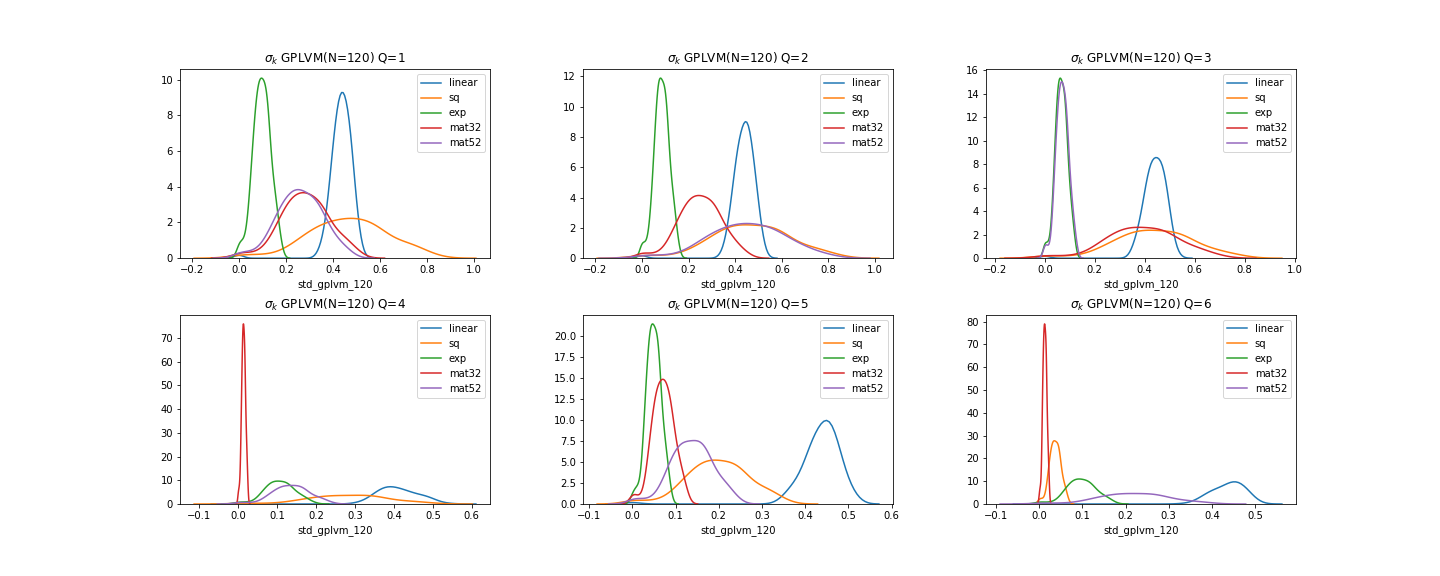
\includegraphics[width=7in]{img/07_0/std_GPLVM_120.png}
	\caption[Standard Deviation Distributions GPLVM]
	{Distributions of vector elements of $\sigma_k$. These values represent volatility in a financial context.}
	\label{fig:gplvm_variances}
\end{figure}
In figure \ref{fig:gplvm_variances} the variances are shown. These are estimated once for each stock, and then kept constant over time. The linear kernel is observed to more often need a higher volatility to function, even though it was outperformed by the other kernels. \newline
Similarly, the entries of the inferred covariance matrix entries' distribution can be plotted, like in figure \ref{fig:gplvm_covariances}. They resemble the statistical connection between two stocks, and should also be $\in\mathbb{R}_0^+$. This is due to covariance matrices, by definition, being positive semi-definite. Also having many entries $>1$ seems improbable, since that would imply a covariance of very great degree, in turn implying a correlation of an unusually high degree. A very large part of the values is close to 0, implying a sane model. 
\begin{figure}%Covariance matrices sanity checks
	\centering
	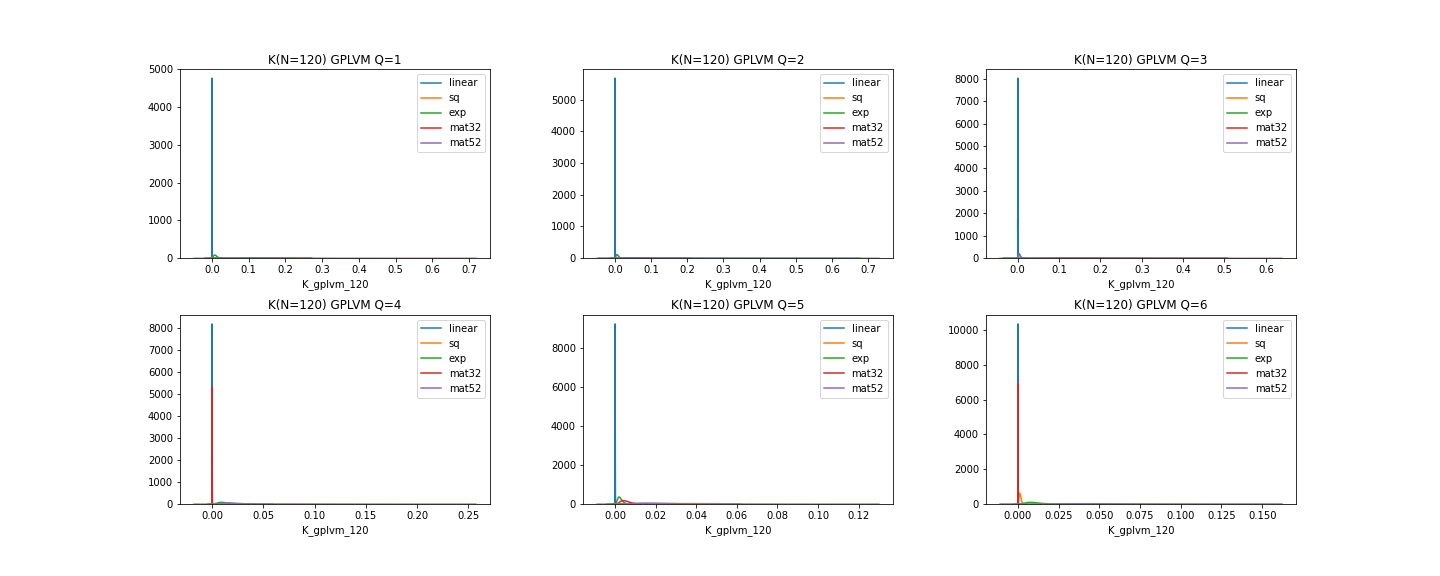
\includegraphics[width=7in]{img/07_0/K_GPLVM_120.png}
	\caption[Covariance Matrix Entry Distributions GPLVM]
	{Distributions of the values of the entries of the covariance matrices. }
	\label{fig:gplvm_covariances}
\end{figure}
After considering the sanity of the model compared to the expectations that can be deduced from observations of reality, different hypotheses can be formulated to explain the deviance from the expectation in the data-prediction-pair plot \ref{fig:gplvm_pair_plot_central}. At first, the effects of the size of the data matrices used to train the model were considered. For this, the size of the data matrix was scaled to include data matrices with different numbers of stocks, and different time periods over which the observations have taken place. We therefore look at different types of flaunty behaviour in the reconstruction, comparing figures \ref{fig:gplvm_N20_pairs}, \ref{fig:gplvm_N60_pairs}, \ref{fig:gplvm_N100_pairs} and \ref{fig:gplvm_N120_pairs}, which show typical behaviour of data-prediction pair plots for $N=20$ \ref{fig:gplvm_N20_pairs}, $N=60$ \ref{fig:gplvm_N60_pairs}, $N=100$ \ref{fig:gplvm_N100_pairs}, and $N=120$ \ref{fig:gplvm_N120_pairs}. 
\begin{figure}%fig:gplvm_N20_pairs
	\centering
	\begin{subfigure}[l]{0.3\textwidth}
		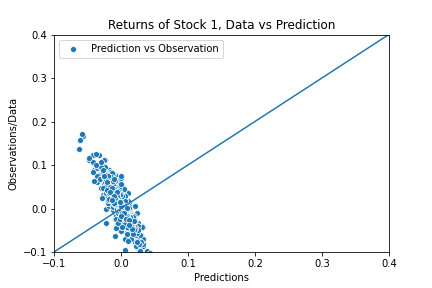
\includegraphics[width=\textwidth]{img/07_0/N20/Q3_kernel3_stock1_scatter.png}
	\end{subfigure}
	\begin{subfigure}[c]{0.3\textwidth}
		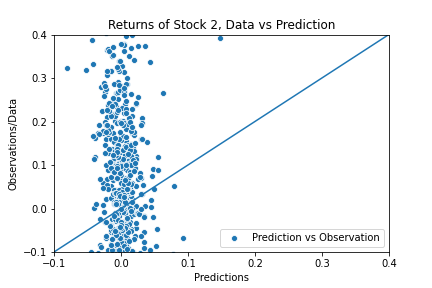
\includegraphics[width=\textwidth]{img/07_0/N20/Q3_kernel3_stock2_scatter.png}
	\end{subfigure}
	\begin{subfigure}[r]{0.3\textwidth}
		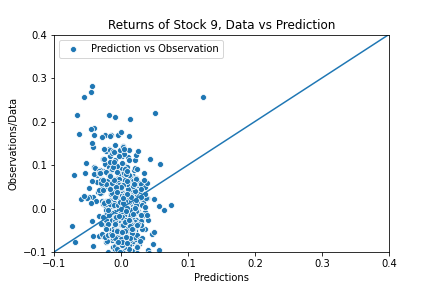
\includegraphics[width=\textwidth]{img/07_0/N20/Q3_kernel3_stock9_scatter.png}
	\end{subfigure}
	\caption[Y-$\hat{Y}$ pair plots for N=20 with the GPLVM model]{Plots from the GPLVM reconstruction with the $N=20$, $D=754$ dataset. The reconstruction failed, but the model had a fast convergence in distributions. }
	\label{fig:gplvm_N20_pairs}
\end{figure}
\begin{figure}%fig:gplvm_N60_pairs
	\centering
	\begin{subfigure}[l]{0.3\textwidth}
		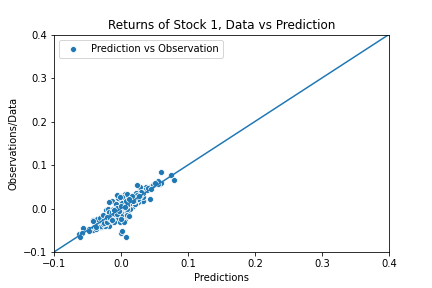
\includegraphics[width=\textwidth]{img/07_0/N60/Q1_kernel1_stock1_scatter.png}
	\end{subfigure}
	\begin{subfigure}[c]{0.3\textwidth}
		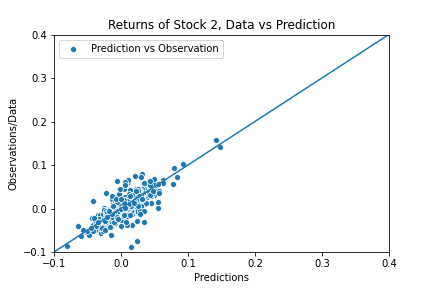
\includegraphics[width=\textwidth]{img/07_0/N60/Q1_kernel1_stock2_scatter.png}
	\end{subfigure}
	\begin{subfigure}[r]{0.3\textwidth}
		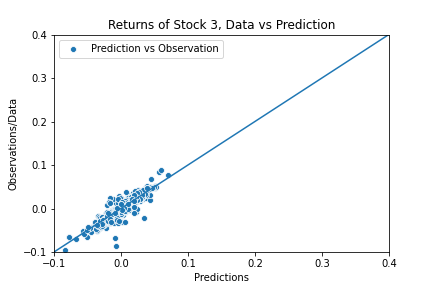
\includegraphics[width=\textwidth]{img/07_0/N60/Q1_kernel1_stock3_scatter.png}
	\end{subfigure}
	\caption[Y-$\hat{Y}$ pair plots for N=60 with the GPLVM model]{Plots from the GPLVM reconstruction with the $N=60$, $D=754$ dataset. The reconstruction worked properly. }
	\label{fig:gplvm_N60_pairs}
\end{figure}
\begin{figure}%fig:gplvm_N100_pairs
	\centering
	\begin{subfigure}[l]{0.3\textwidth}
		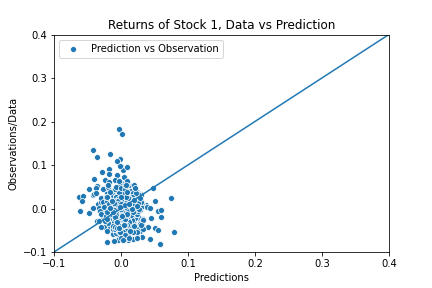
\includegraphics[width=\textwidth]{img/07_0/N100/Q1_kernel1_stock1_scatter.png}
	\end{subfigure}
	\begin{subfigure}[c]{0.3\textwidth}
		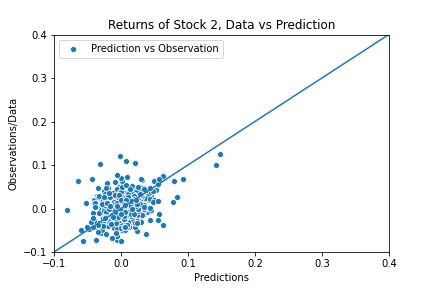
\includegraphics[width=\textwidth]{img/07_0/N100/Q1_kernel1_stock2_scatter.png}
	\end{subfigure}
	\begin{subfigure}[r]{0.3\textwidth}
		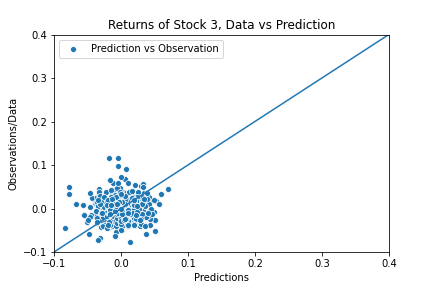
\includegraphics[width=\textwidth]{img/07_0/N100/Q1_kernel1_stock3_scatter.png}
	\end{subfigure}
	\caption[Y-$\hat{Y}$ pair plots for N=100 with the GPLVM model]{Plots from the GPLVM reconstruction with the $N=60$, $D=754$ dataset. The circular shape of the cloud indicates that the distributions of $Y$ and $\hat{Y}$ are well fit, but subpar reconstruction.}
	\label{fig:gplvm_N100_pairs}
\end{figure}
\begin{figure}%fig:gplvm_N120_pairs
	\centering
	\begin{subfigure}[l]{0.3\textwidth}
		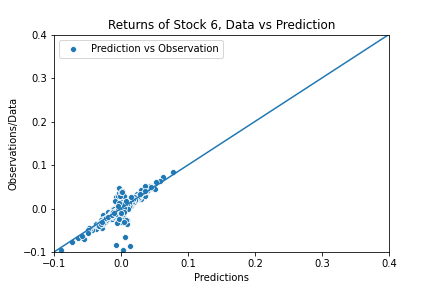
\includegraphics[width=\textwidth]{img/07_0/N120/Q1_kernel3_stock6_scatter.png}
	\end{subfigure}
	\begin{subfigure}[c]{0.3\textwidth}
		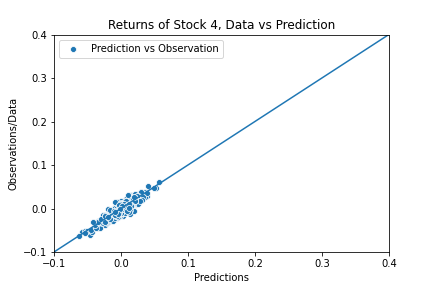
\includegraphics[width=\textwidth]{img/07_0/N120/Q6_kernel1_stock4_scatter.png}
	\end{subfigure}
	\begin{subfigure}[r]{0.3\textwidth}
		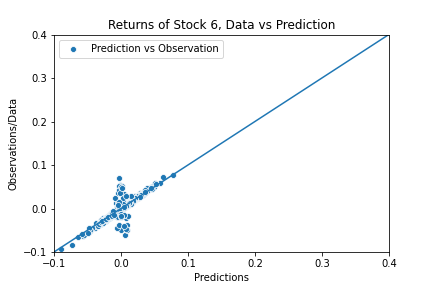
\includegraphics[width=\textwidth]{img/07_0/N120/Q3_kernel5_stock6_scatter.png}
	\end{subfigure}
	\caption[Y-$\hat{Y}$ pair plots for N=120 with the GPLVM model]{Plots from the GPLVM reconstruction with the $N=60$, $D=754$ dataset. We can find a good estimation of the true posterior, and a good reconstruction, but also find that in some cases, to match the data distribution some predictions are very close to 0, not representing the data at all.}
	\label{fig:gplvm_N120_pairs}
\end{figure} 
From this we can conclude, that the model has an intrinsic error reconstructing the covariance structure while still matching the target 1D-distributions of the data. In the following part of this chapter, different possible solutions to this problem are discussed. 
%%
%VOLATILITY CORRECTED GPLVM
%%
\subsection{Volatility normalized datasets}
Since the GPLVM model does not have time dependent volatility, different possible scenarios can not be incorporated into the model. For example, stocks with comparably high, but also highly varying volatility will not be represented very well, since the model will probably infer the mean volatility for this value. Therefore, the model was also tested against datasets where the stocks were normalized (VN - Volatility normalized) one by one, using the inferred volatility of a HCMC optimized GARCH process, compare sections \ref{sec:arch} and \ref{sec:mcmc}, as well as \cite{pyflux}. The results are again depicted through example pictures of the systematic deviation observed in the $Y-\hat{Y}$-pair plots. Also, sanity checks were performed, e.g. plotting noises and variances. Here, since the expected volatility was used to normalize the returns on their respective predicted volatilities, the variance in figure \ref{fig:variance_vcr} should be close to zero. This aspect was recognized correctly by the model. The inherent noise should be small, and is shown in \ref{fig:noise_vcr}. These figures also show, that the calculation does not resemble correctly our expectations of the model. Also, we acknowledge that another prior distribution would have been a better suited choice, since the kernel density estimate plots show values smaller than 0, which are forbidden through the generating process chosen. 
\begin{figure}[h!]
	\centering
	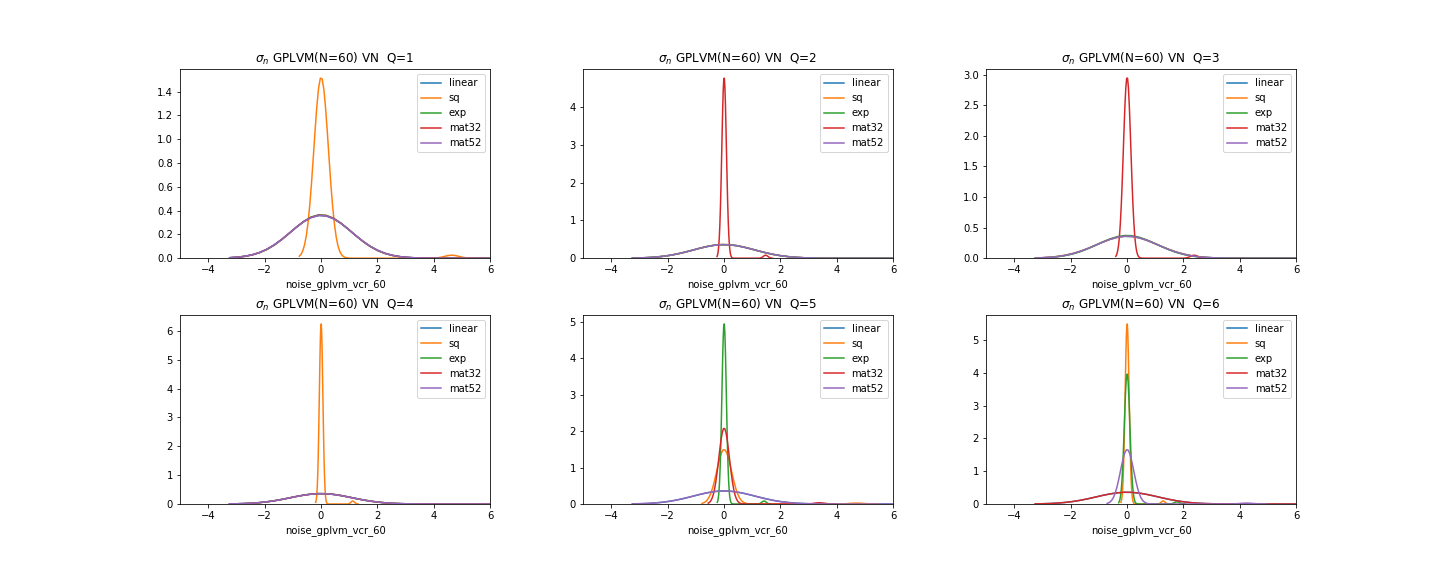
\includegraphics[width=7in]{img/07_0/noise_GPLVM_vcr_60.png}
	\caption[Noise Distribution of GPLVM with VCR dataset]{Distributions of $\sigma_{n}$, which were trained on a VN dataset with $N=60$ and $D=125$.}
	\label{fig:noise_vcr}
\end{figure}
\begin{figure}[h!]%fig:noise_variance_vcr
	\centering
	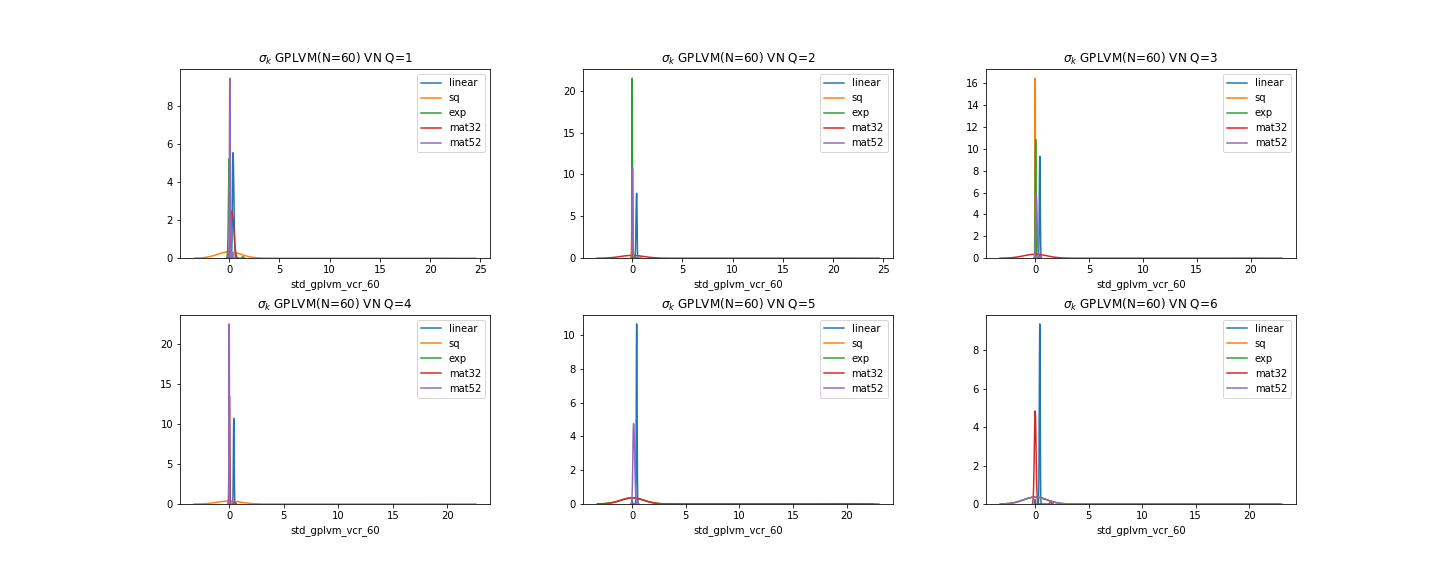
\includegraphics[width=7in]{img/07_0/std_GPLVM_vcr_60.png}
	\caption[Variance Distributions of GPLVM with VN dataset]{Distributions of $\sigma_{n}$, which were trained on a VN dataset with $N=60$ and $D=125$.}
	\label{fig:variance_vcr}
\end{figure}
Since we found a dependency on the size of the data matrix $Y$, we test the model with different sizes of datasets, shown in figure \ref{fig:dataset_size_init}. We recorded which sizes of data sets, within the confinement of the largest data set of $N=120$ and $D=754$, would successfully run without stan rejecting the initial values due to bad conditioning. Stan uses several hundreds of initial values for initialization. An orange dot is used if the model did not initialize. If the model did initialize, a blue dot is used. All experiments were carried out using a squared exponential kernel and using $Q=3$ latent dimensions.
\begin{figure}[h!]%Initializable Y-sizes with the GARCH-volatility-corrected dataset sizes. 
	\centering
	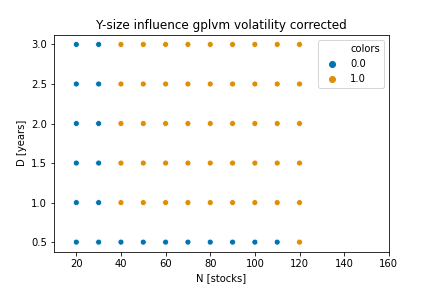
\includegraphics[width=4in]{img/07_0/size_influence-gplvm_vcr.png}
	\caption[Initialization of GPLVM model VN datasets]
	{Shown here, in the same style as with the regular datasets and the GPLVM-model is the influence of dataset sizes on initialization. Again, blue points represent input matrix sizes, that were successfully initialized, while orange points represent matrix sizes, where initialization failed.}
	\label{fig:dataset_size_init}
\end{figure}
We observe that the data sets that initialized successfully were either over very short time frames, or with very little stocks. We conclude therefore, that the used GARCH process breaks down for longer time frames due to errors propagating, as well as for more observed stocks, which reflect a more complicated part of the true covariance structure. In comparison, experiments showed that the regular, unnormalized, data set always initialized properly. \newline \newline
The example data set evaluated was $N=60$, $D=125$. It showed a range of behaviors when reproducing the data. Examples of these behaviors are shown in figures \ref{fig:gplvm_vcr_pairs}, where the model does a very good fit (\textit{left}), reproduces a very bad fit (\textit{center}), and shows the property to reproduce a correct target distribution but not with the right data points (\textit{right}). These pitfalls have also been seen before, in the GPLVM model, especially figures \ref{fig:gplvm_N20_pairs}, \ref{fig:gplvm_N100_pairs}, and \ref{fig:gplvm_N120_pairs}. The suspicion therefore arises, that normalizing the dataset either went wrong, or destroyed the overall covariance structure in such a way, that the model could not reconstruct it. 
\begin{figure}%fig:gplvm_N120_pairs
	\centering
	\begin{subfigure}[l]{0.2\textwidth}
		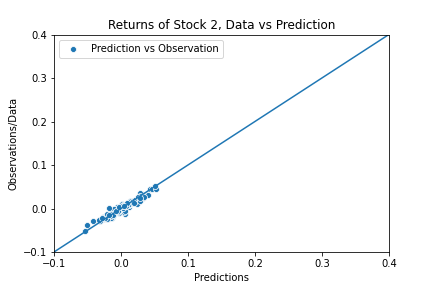
\includegraphics[width=\textwidth]{img/07_0/N60D123/Q1_kernel1_stock2_scatter.png}
	\end{subfigure}
	\begin{subfigure}[c]{0.3\textwidth}
		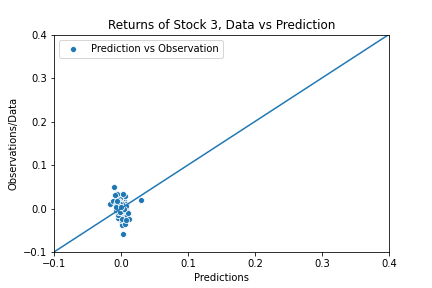
\includegraphics[width=\textwidth]{img/07_0/N60D123/Q1_kernel1_stock3_scatter.png}
	\end{subfigure}
	\begin{subfigure}[r]{0.3\textwidth}
		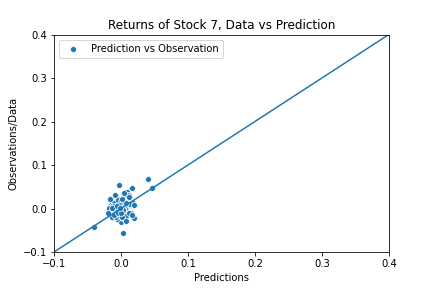
\includegraphics[width=\textwidth]{img/07_0/N60D123/Q1_kernel1_stock7_scatter.png}
	\end{subfigure}
	\caption[Y-$\hat{Y}$ pair plots for $N=60$, $D=125$ VN-data with the GPLVM model]{Plots from the GPLVM reconstruction with the $N=60$, $D=754$ dataset. We can find a good estimation of the true posterior, and a good reconstruction, but also find that in some cases, to match the data distribution some predictions are very close to 0, not representing the data at all.}
	\label{fig:gplvm_vcr_pairs}
\end{figure}
\label{res:gplvm}
\cleardoubleoddpage

\section{Student-t Process Latent Variable Model}
The Student-t Latent Variable Model (SPLVM) is based upon the notion that a Student-t process can more accurately fit data with a higher percentage of outliers due to broader flanks. This, in theory resembles a higher volatility, but it is not directly implemented into the model. Overall, expectations are, that the higher robustness towards outliers will improve upon the results of the GPLVM. \newline \newline
First, we implement the model, similar to the GPLVM model, but using a function that solves the model using multivariate Student-t distributions. Compare the model code in Appendix \ref{sec:model_code}. Analyzing the closed form solutions described in \ref{sec:student-t}, we find that the Student-t process will behave like the GPLVM, but with an additional multiplicative term giving more flexibility to the covariance matrix. Also, we observe that a Student-t process will become a Gaussian Process for the degree of freedom parameter $\nu \to \infty$, the evaluation of $\nu$ will be particularly interesting for interpretation. It can solve the question of whether a Gaussian process ($\nu \to \infty$), a Student-t Process ($\nu \in [2,\infty)$) solve the problem best, and even show tendencies since the interval is defined over all possible values for $\nu \in \mathbb{R}_0^+$. A rule of thumb in practice is, that from a value of $\nu \geq 30$ on, the Student-t distribution is sufficiently well approximated by a Gaussian distribution. 
The optimal inferred values of $\nu$ are shown in table \ref{tab:splvm_nu}, for the calculations the same input sizes are used as in the main GPLVM run, $N=120$, $D=754$. 
\begin{table}
    \centering
	\begin{tabular}{||l|r|r|r|r|r|r||}\hline
		$\nu$     & Q1        &  Q2       & Q3        & Q4        & Q5        & Q6        \\ \hline
		lin       &  8.847574 &  2.006339 &  2.001937 &  8.651835 &  2.007558 &  2.002983 \\
		exp       &  2.008647 &  2.003451 &  2.009492 &  2.003444 &  2.003168 &  2.001988 \\
		exp2      &  2.002464 &  2.007803 &  2.002753 &  8.199555 &  2.001955 &  2.009912 \\
		mat32     &  8.351861 &  2.002681 &  2.002718 &  2.003437 &  2.006565 &  2.009912 \\
		mat52     &  2.002612 &  2.011853 &  2.004670 &  2.002371 &  2.003071 &  2.001988 \\ \hline
	\end{tabular}
	\label{tab:splvm_nu}
\end{table}
Therefore, we can conclude temporarily that A more Student-t like stochastic process is probably better suited. We find the results of the Student-t model as figure \ref{fig:studt_ELBO_R2}, further exemplifying the notion that the Student-t process is better suited, if not by much. Again, the same holds as with the GPLVM, where the linear kernel underperforms, and higher numbers of latent dimensions perform better. 
\begin{figure}%fig:studt_ELBO_R2      ELBO/R2 values of SPLVM
	\centering
	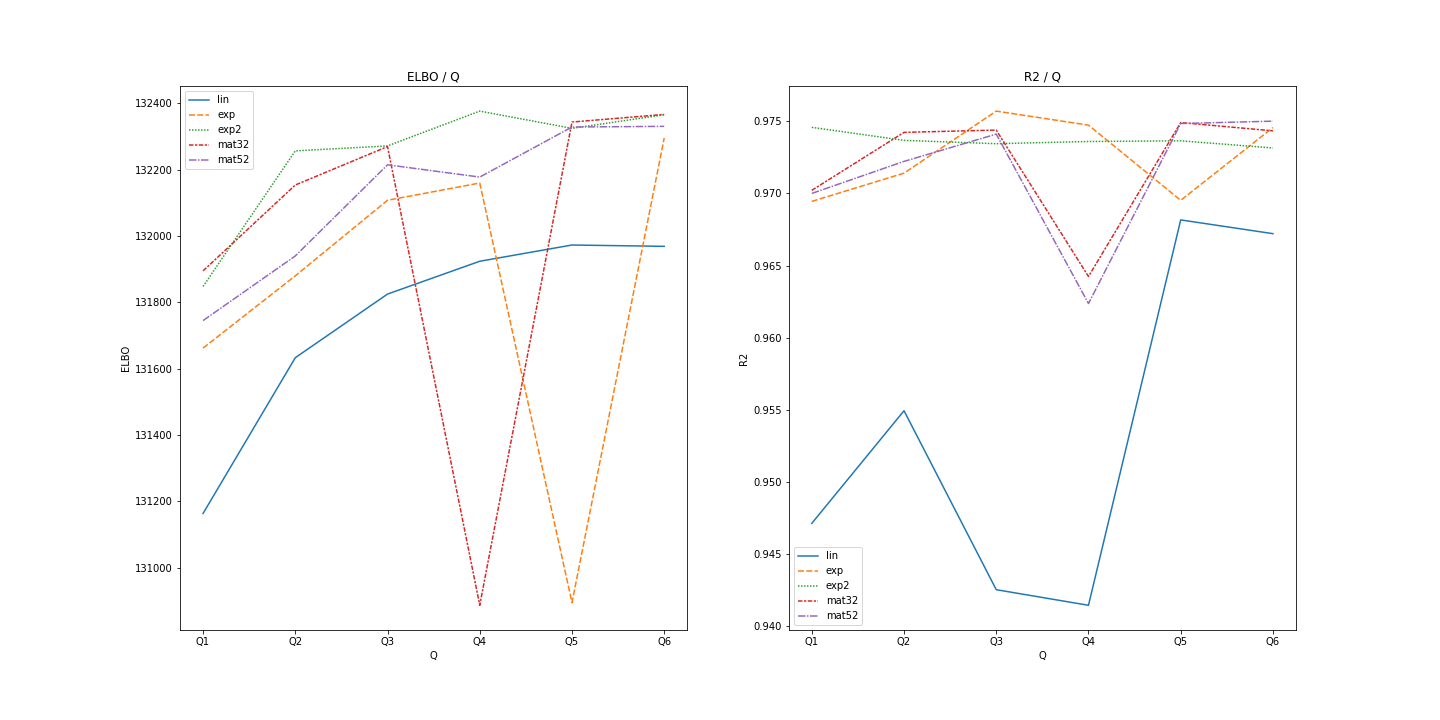
\includegraphics[width=4in]{img/07_1/modelSTUDT_Qs.png}
	\caption[SPLVM ELBO and $R^2$ values for the $N=120$, $D=754$ dataset.]{ELBO and R2 values of the Student-t Process Latent Variable Model (SPLVM).}
	\label{fig:studt_ELBO_R2}
\end{figure}
The distributions of intercept values and slope values of the 120 stocks are shown in figures \ref{fig:studt_intercepts} and \ref{fig:studt_slopes}. Here, we see that the SPLVM model again performs slightly better than the GPLVM. We attribute this performance increase to the broader flanks of the Student-t distribution. Therefore, the outliers seem to be a problem. This does not explain which influences result in those outliers. 
\begin{figure}%fig:studt_intercepts      SPLVM Intercept distributions
	\centering
	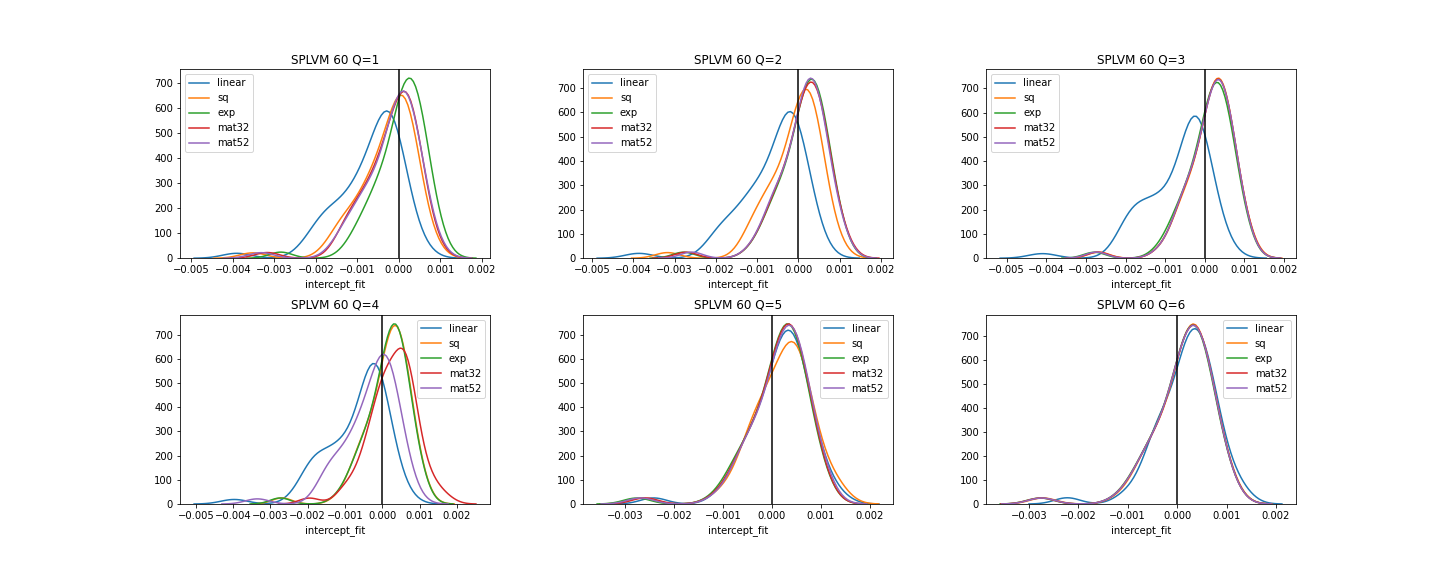
\includegraphics[width=7in]{img/07_1/intercept_fit_studt_120.png}
	\caption[SPLVM intercept values for $N=120$, $D=754$]{The distributions of the intercept values, which should be centered around the vertical line at $x=0$. }
	\label{fig:studt_intercepts}
\end{figure}
\begin{figure}%fig:studt_slopes      SPLVM Slope distributions
	\centering
	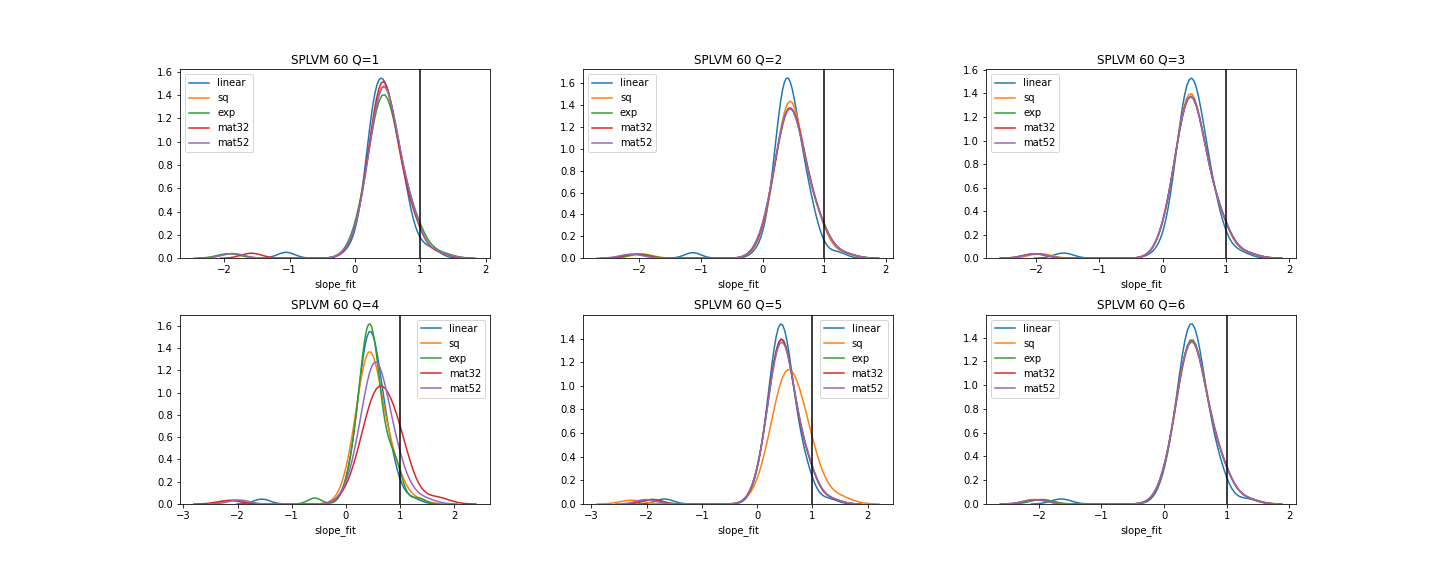
\includegraphics[width=7in]{img/07_1/slope_fit_studt_120.png}
	\caption[SPLVM slope values for $N=120$, $D=754$]{The distributions of the slope values, which should be centered around the left of the vertical line at $x=1$. }
	\label{fig:studt_slopes}
\end{figure}
Just as the GPLVM model, the SPLVM model initializes with any regular data set size, the noticeable difference here, is that it performs so much worse with the VN data sets, that it did not initialize at all. This leads to the assumption, that the volatility does contribute into the broader flanks of the Student-t distribution. Also, we conclude the same sanity checks as before in section \ref{res:gplvm}, looking at the noise and the variance entries. Figures \ref{fig:studt_noises} and \ref{fig:studt_variances} show that for all models, the noise and variance entries show no erroneous behavior. 
\begin{figure}%fig:studt_noises
	\centering
	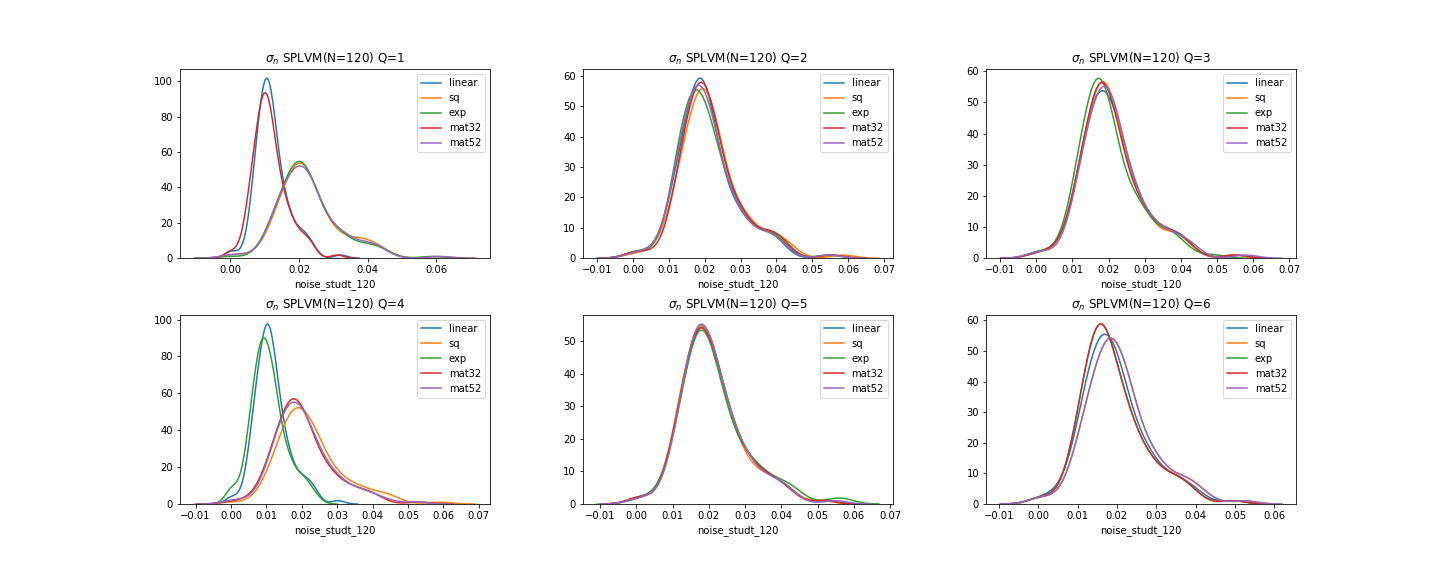
\includegraphics[width=7in]{img/07_1/noise_STUDT_120.png}
	\caption[SPLVM noise values for $N=120$, $D=754$]{The distributions of values of the vector $\sigma_n$. }
	\label{fig:studt_noises}
\end{figure}
\begin{figure}%fig:studt_variances
	\centering
	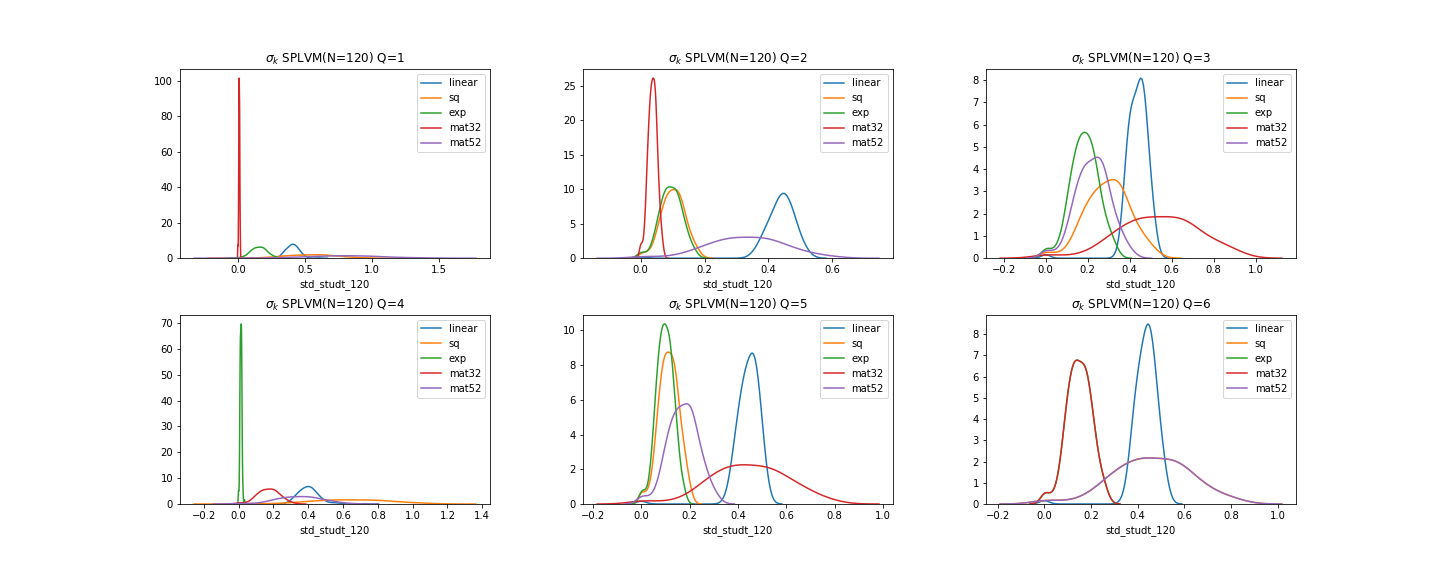
\includegraphics[width=7in]{img/07_1/std_STUDT_120.png}
	\caption[SPLVM variance values for $N=120$, $D=754$]{The distributions of values of the vector containing the variances.}
	\label{fig:studt_variances}
\end{figure}
The dependence of the SPLVM model on the size of data set was also determined by looking at different erroneous behaviors of reconstruction of the data, in figures \ref{fig:studt_N20_pairs}, \ref{fig:studt_N60_pairs}, \ref{fig:studt_N100_pairs} and \ref{fig:studt_N120_pairs}. Overall we observe that the systematic error observed in the GPLVM model results is lessened by applying the Student-t model to the same problem. 
\begin{figure}%fig:gplvm_N20_pairs
	\centering
	\begin{subfigure}[l]{0.3\textwidth}
		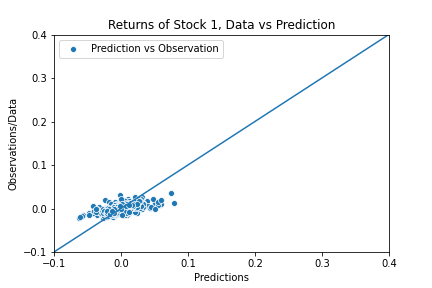
\includegraphics[width=\textwidth]{img/07_1/N20/Q1_kernel1_stock1_scatter.png}
	\end{subfigure}
	\begin{subfigure}[c]{0.3\textwidth}
		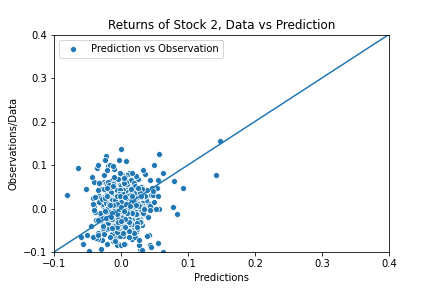
\includegraphics[width=\textwidth]{img/07_1/N20/Q1_kernel1_stock2_scatter.png}
	\end{subfigure}
	\begin{subfigure}[r]{0.3\textwidth}
		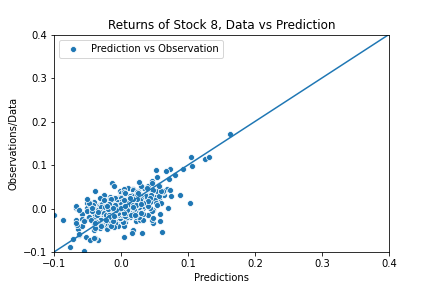
\includegraphics[width=\textwidth]{img/07_1/N20/Q1_kernel1_stock8_scatter.png}
	\end{subfigure}
	\caption[Y-$\hat{Y}$ pair plots for N=20 with the SPLVM model]{Plots from the SPLVM reconstruction with the $N=20$, $D=754$ dataset. The reconstruction failed showing the circular correct reconstruction of a 1D representation of the distribution of data points.}
	\label{fig:studt_N20_pairs}
\end{figure}
\begin{figure}%fig:gplvm_N60_pairs
	\centering
	\begin{subfigure}[l]{0.3\textwidth}
		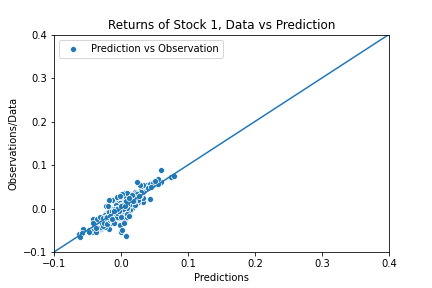
\includegraphics[width=\textwidth]{img/07_1/N60/Q1_kernel1_stock1_scatter.png}
	\end{subfigure}
	\begin{subfigure}[c]{0.3\textwidth}
		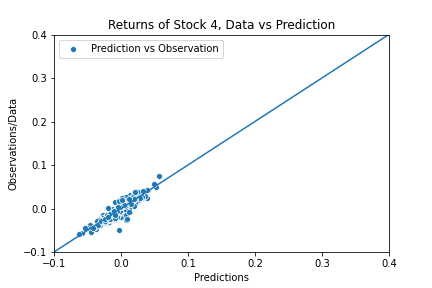
\includegraphics[width=\textwidth]{img/07_1/N60/Q1_kernel1_stock4_scatter.png}
	\end{subfigure}
	\begin{subfigure}[r]{0.3\textwidth}
		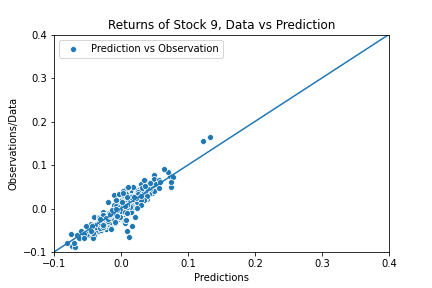
\includegraphics[width=\textwidth]{img/07_1/N60/Q1_kernel1_stock9_scatter.png}
	\end{subfigure}
	\caption[Y-$\hat{Y}$ pair plots for N=60 with the SPLVM model]{Plots from the SPLVM reconstruction with the $N=60$, $D=754$ dataset. The reconstruction worked properly. }
	\label{fig:studt_N60_pairs}
\end{figure}
\begin{figure}%fig:gplvm_N100_pairs
	\centering
	\begin{subfigure}[l]{0.3\textwidth}
		\includegraphics[width=\textwidth]{img/07_1/N100/Q1_kernel1_stock1_scatter.png}
	\end{subfigure}
	\begin{subfigure}[c]{0.3\textwidth}
		\includegraphics[width=\textwidth]{img/07_1/N100/Q1_kernel1_stock2_scatter.png}
	\end{subfigure}
	\begin{subfigure}[r]{0.3\textwidth}
		\includegraphics[width=\textwidth]{img/07_1/N100/Q1_kernel1_stock3_scatter.png}
	\end{subfigure}
	\caption[Y-$\hat{Y}$ pair plots for N=100 with the SPLVM model]{Plots from the SPLVM reconstruction with the $N=60$, $D=754$ dataset. The circular shape of the cloud indicates that the distributions of $Y$ and $\hat{Y}$ are well fit, but subpar reconstruction of the data has taken place.}
	\label{fig:studt_N100_pairs}
\end{figure}
\begin{figure}%fig:gplvm_N120_pairs
	\centering
	\begin{subfigure}[l]{0.3\textwidth}
		\includegraphics[width=\textwidth]{img/07_1/N120/Q1_kernel1_stock1_scatter.png}
	\end{subfigure}
	\begin{subfigure}[c]{0.3\textwidth}
		\includegraphics[width=\textwidth]{img/07_1/N120/Q1_kernel1_stock4_scatter.png}
	\end{subfigure}
	\begin{subfigure}[r]{0.3\textwidth}
		\includegraphics[width=\textwidth]{img/07_1/N120/Q1_kernel1_stock5_scatter.png}
	\end{subfigure}
	\caption[Y-$\hat{Y}$ pair plots for N=120 with the SPLVM model]{Plots from the SPLVM reconstruction with the $N=60$, $D=754$ dataset. We can find a good estimation of the true posterior, and a good reconstruction, while the off-diagonal that was observed with the GPLVM model is sufficiently smaller. }
	\label{fig:studt_N120_pairs}
\end{figure} 
\label{res:splvm}
\cleardoubleoddpage

\section{Volatility GPLVM}
The Volatility GPLVM (V-GPLVM) model is a generalization of the GPLVM model, as discussed in section \ref{sec:models}, where the volatility is reinterpreted as a time dependent quantity. Using the equations and generating process from section \ref{sec:v_gplvm}, we arrive at the model code found in \ref{sec:model_code}. Due to the large number of parameters that need to be stored in RAM at a time, the size of the data matrix $Y$ had to be sufficiently smaller, $Y\in\mathbb{R}^{N,D}=\mathbb{R}^{10,250}$. We find that the model does not apply well to the data, which can be seen from the kernel density estimates of the distributions of noise ($\sigma_n$) and variance ($\Sigma$) values in figures \ref{fig:vola_noises} and \ref{fig:vola_variances}. These estimates should not be having large parts of the estimation reach be outside $\mathbb{R}_0^+$, as this is forbidden by design. In addition, the values should not center around 1, again solidifying the evidence of a corrupted model. Also note, that 
\begin{equation}%eq:variance_volatility
	\Sigma \propto \log(\Sigma_V),
	\label{eq:variance_volatility}
\end{equation}
the variance $\Sigma$ is proportional to the logarithm of the volatility $\log(\Sigma_V)$. The values of the covariance entries, which mainly lie at value $1$ suggest, that the model finds and stays in a steep local minima on the energy surface, which seems unshirkable. It does not seem to be the global minimum though, since covariance entry values, ELBO values and $R^2$ values are far off from where we would expect them to be \ref{fig:vola_ELBO_R2}. We again see that the linear kernel under performs significantly, especially when looking at the volatility values, which need to be way higher, or even unreasonably high for the under performing model. More sophisticated kernels perform better in all tests, and again higher numbers of latent dimensions perform better than lower numbers. If we look at the results, we again can conclude, that not even all model specifications have landed securely in the suspected local minimum due to major differences in ELBO values and $R^2$ values. Also, the $R^2$ values shown in \ref{fig:vola_ELBO_R2} lead to the wrong conclusion, since they only can compare lower dimensional representations of the distributions. 
\begin{figure}[t]%fig:vola_noises
	\centering
	\includegraphics[width=7in]{img/07_2/noise_VOLA_elbo.png}
	\caption[V-GPLVM noise distributions]{V-GPLVM noise distributions for the $N=10$, $D=250$ data set.}
	\label{fig:vola_noises}
\end{figure}
\begin{figure}[b]%fig:vola_variances
	\centering
	\includegraphics[width=7in]{img/07_2/Sigma_VOLA_elbo.png}
	\caption[V-GPLVM Variance distributions]{V-GPLVM Variance distributions for the $N=10$, $D=250$ data set.}
	\label{fig:vola_variances}
\end{figure}
\begin{figure}[t]
	\centering
	\includegraphics[width=7in]{img/07_2/modelVOLA_Qs.png}
	\caption[V-GPLVM ELBO and $R^2$ model results]{ELBO and R2 values grouped by number of latent dimensions ($Q$) for the V-GPLVM model.}
	\label{fig:vola_ELBO_R2}
\end{figure}
Due to the differences in size in $Y$, these results can not be compared to the GPLVM results directly, but indirectly through looking at the behavior of the model reconstructing the input data in figures \ref{fig:vola_N10_pairs}. These plots again show the same erroneous behavior as the GPLVM model, with a lot of stocks being represented with circle-like shape (\textit{left}) that reproduces the distribution well, but does not reconstruct the higher dimensional representation of the pair plot correctly. This behavior can e.g. inflate $R^2$ values, misleading the reader. The \textit{center} frame shows the erroneous behavior found in the GPLVM model, where to match the distributions, some predictions are falsely set to 0. 
\begin{figure}[b]%fig:vola_N10_pairs
	\centering
	\begin{subfigure}[l]{0.3\textwidth}
		\includegraphics[width=\textwidth]{img/07_2/elbo/Q1_kernel1_stock1_scatter.png}
	\end{subfigure}
	\begin{subfigure}[c]{0.3\textwidth}
		\includegraphics[width=\textwidth]{img/07_2/elbo/Q1_kernel1_stock9_scatter.png}
	\end{subfigure}
	\begin{subfigure}[r]{0.3\textwidth}
		\includegraphics[width=\textwidth]{img/07_2/elbo/Q1_kernel1_stock2_scatter.png}
	\end{subfigure}
	\caption[Y-$\hat{Y}$ pair plots V-GPLVM model]{Y-$\hat{Y}$ pair plots with the V-GPLVM model $N=10$, $D=250$.}
	\label{fig:vola_N10_pairs}
\end{figure}
Also, we can observe the behavior of the model simply underestimating high returns and overestimating low returns, so that the intercept is far off the desired value of 1. This leads directly to the slope, figure \ref{fig:vola_slopes}, and intercept, figure \ref{fig:vola_intercepts}, distributions of the V-GPLVM model. 
\begin{figure}[t]%fig:vola_slopes
	\centering
	\includegraphics[width=7in]{img/07_2/slope_fit_vola_elbo.png}
	\caption[V-GPLVM slopes distributions]{V-GPLVM slopes distributions for the $N=10$, $D=250$ data set.}
	\label{fig:vola_slopes}
\end{figure}
\begin{figure}[b]%fig:vola_intercepts
	\centering
	\includegraphics[width=7in]{img/07_2/intercept_fit_vola_elbo.png}
	\caption[V-GPLVM intercepts distributions]{V-GPLVM intercept distributions for the $N=10$, $D=250$ data set.}
	\label{fig:vola_intercepts}
\end{figure}
Again, the model did not initialize sufficiently well with the volatility normalized data sets, as to provide an interpretation. Compared to the other models previously discussed, the slope and intercept distributions giving a quick overview of all the different possible Y-$\hat{Y}$-pair plots, are far off from the optimum. Therefore, we conclude that the model, even though not explicitly comparable, does not measure up with the previous models. 
\label{res:vola}
\cleardoubleoddpage

\section{Time-dependent Latent Space GPLVM}
The Time-dependent Latent Space GPLVM model allows the GPLVM extra flexibility through the stocks representations in latent space having mobility. The distance between the instances in latent space implies higher correlation if it is smaller, and lower correlation if it is larger. We proceed with the same sanity checks and model evaluations as before. It is necessary to note, that the model did not produce symmetric covariance matrices for kernels of the Matern-class. Therefore, these are not part of the evaluation. Also, due to the size of the matrices needed to express this model, only the small data matrix that was used in the V-GPLVM ($N=10$, $D=250$) could be used. 
\begin{figure}[t]
	\centering
	\includegraphics[width=7in]{img/07_3/noise_time_elbo.png}
	\caption[T-GPLVM noise distributions]{T-GPLVM data space ($Y$) observation noise distributions.}
	\label{fig:tgplvm_noise}
\end{figure}
\begin{figure}[b]
	\centering
	\includegraphics[width=7in]{img/07_3/std_time_elbo.png}
	\caption[T-GPLVM variance distributions]{T-GPLVM data space ($Y$) variance distributions.}
	\label{fig:tgplvm_variance}
\end{figure}
\begin{figure}[t]
	\centering
	\includegraphics[width=7in]{img/07_3/K_time_elbo.png}
	\caption[T-GPLVM covariance matrix entries distributions]{Covariance matrix entries distributions from the T-GPLVM model run.}
	\label{fig:tgplvm_covariance}
\end{figure}
Figure \ref{fig:tgplvm_noise} shows good agreement with expectations, observation noise is comparably low for all different versions of the model. On the other hand figure \ref{fig:tgplvm_variance}, displaying the variance, shows erroneous behavior, and probably would have been better approximated with some other, most likely asymmetric distribution. At last figure \ref{fig:tgplvm_covariance} shows values close to 0 dominating, implying comparably small covariance between stocks.
\begin{figure}[b]
	\centering
	\includegraphics[width=7in]{img/07_3/modelTIME_Qs.png}
	\caption[T-GPLVM ELBO and $R^2$ results]{ELBO and $R^2$ values from the T-GPLVM model run, without the Matern class kernels.}
	\label{fig:tgplvm_ELBO_R2}
\end{figure}
Figure \ref{fig:tgplvm_ELBO_R2} then provides a problem of interpretation. While the ELBO values of the linear kernel are lower, the lower dimensional representation of the reconstruction in form of the $R^2$ values is considerably higher for the linear kernel. Overarching still is the fact, that the ELBO values and $R^2$ values still can not compete with the GPLVM model, just like the V-GPLVM model. 
\begin{figure}[t]
	\centering
	\includegraphics[width=7in]{img/07_3/slope_fit_time_elbo.png}
	\caption[T-GPLVM slope distributions]{Distributions of slopes from the Y-$\hat{Y}$ pairs for the T-GPLVM model.}
	\label{fig:tgplvm_slopes}
\end{figure}
\begin{figure}[b]
	\centering
	\includegraphics[width=7in]{img/07_3/intercept_fit_time_elbo.png}
	\caption[T-GPLVM intercept distributions]{Distributions of intercepts from the Y-$\hat{Y}$ pairs for the T-GPLVM model.}
	\label{fig:tgplvm_intercepts}
\end{figure}
This conclusion is further exemplified in figures \ref{fig:tgplvm_slopes} and \ref{fig:tgplvm_slopes}, where intercepts can compete with the other models, but slopes of the Huber regression still produce distributions with values so far off from the desired value. Last, but not least, evaluating some examples of the Y-$\hat{Y}$-pair plots makes abundantly clear, that the model still has issues in need to be fixed. All examples show, that distributions match only in lower dimensional representations. The covariance structure of 10 stocks was not enough to be representative of the underlying structure. 
\begin{figure}[t]%fig:gplvm_N120_pairs
	\centering
	\begin{subfigure}[l]{0.3\textwidth}
		\includegraphics[width=\textwidth]{img/07_3/Q1_kernel1_stock1_scatter.png}
	\end{subfigure}
	\begin{subfigure}[c]{0.3\textwidth}
		\includegraphics[width=\textwidth]{img/07_3/Q1_kernel1_stock2_scatter.png}
	\end{subfigure}
	\begin{subfigure}[r]{0.3\textwidth}
		\includegraphics[width=\textwidth]{img/07_3/Q2_kernel1_stock4_scatter.png}
	\end{subfigure}
	\caption[Y-$\hat{Y}$ pair plots for N=10 with the T-GPLVM model]{Plots from the T-GPLVM reconstruction with the $N=10$, $D=250$ dataset.}
	\label{fig:T-Gplvm_pairs}
\end{figure} 
\label{res:time}
\cleardoubleoddpage

\section{Time-dependent Latent Space SPLVM}
The Time-dependent Latent Space SPLVM model (T-SPLVM) is in comparison to the T-GPLVM what the SPLVM is to the GPLVM. Figure \ref{fig:tsplvm_noise} is showing distributions of the data space observation noise. These plots show healthy behavior, even though some stocks are inferred by the model to have 0 observation noise. 
\begin{figure}
	\centering
	\includegraphics[width=7in]{img/07_4/noise_timet_elbo.png}
	\caption[]{}
	\label{fig:tsplvm_noise}
\end{figure}
Figure \ref{fig:tsplvm_variance} follows, displaying the same unhealthy behavior as the data space process variance did in the T-GPLVM chapter \ref{res:time}. The entries of the covariance matrix then also show unexpected kernel density estimates, ranging to extremely high values. This leads to the conclusion, that the T-SPLVM model still lacks in quality. 
\begin{figure}
	\centering
	\includegraphics[width=7in]{img/07_4/std_timet_elbo.png}
	\caption[]{}
	\label{fig:tsplvm_variance}
\end{figure}
\begin{figure}
	\centering
	\includegraphics[width=7in]{img/07_4/K_timet_elbo.png}
	\caption[]{}
	\label{}
\end{figure}
Checking the ELBO and $R^2$ values, after identifying erroneous behavior is but a formality, still it is easy to see that the model, scoring comparably to the T-GPLVM model, is not able to compete with the GPLVM or SPLVM model. Here, as the initial expectation suggests, the linear kernel performs considerably worse than the more sophisticated kernels. 
\begin{figure}
	\centering
	\includegraphics[width=7in]{img/07_4/modelTIMET_Qs.png}
	\caption[]{}
	\label{fig:tsplvm_ELBO_R2}
\end{figure}
The second to last test of the model, looking at slope and intercept distributions, again proves this model as not competitive. While intercepts, as with all models, are close enough to the desired value of 0 to meet expectations.
\begin{figure}
	\centering
	\includegraphics[width=7in]{img/07_4/slope_fit_timet_elbo.png}
	\caption[]{}
	\label{fig:tsplvm_slopes}
\end{figure}
\begin{figure}
	\centering
	\includegraphics[width=7in]{img/07_4/intercept_fit_timet_elbo.png}
	\caption[]{}
	\label{fig:tsplvm_intercepts}
\end{figure}
The last test of the model, comparing Y-$\hat{Y}$-pair plots \ref{fig:tsplvm_pairs} provides us with the evidence to also not consider this model for further evaluation, showing no behavior close to the expectation. 
\begin{figure}%fig:gplvm_N120_pairs
	\centering
	\begin{subfigure}[l]{0.3\textwidth}
		\includegraphics[width=\textwidth]{img/07_4/timet_elbo/Q1_kernel1_stock1_scatter.png}
	\end{subfigure}
	\begin{subfigure}[c]{0.3\textwidth}
		\includegraphics[width=\textwidth]{img/07_4/timet_elbo/Q1_kernel1_stock6_scatter.png}
	\end{subfigure}
	\begin{subfigure}[r]{0.3\textwidth}
		\includegraphics[width=\textwidth]{img/07_4/timet_elbo/Q4_kernel2_stock8_scatter.png}
	\end{subfigure}
	\caption[Y-$\hat{Y}$ pair plots for N=10 with the T-SPLVM model]{Plots from the SPLVM reconstruction with the $N=10$, $D=250$ dataset.}
	\label{fig:tsplvm_pairs}
\end{figure} 
We find defective behavior to hold for all examples of these plots, in all variants of the model. 
\label{res:timet}
\cleardoubleoddpage
	\label{sec:results}
	
	\chapter{Conclusion and Outlook}
In this thesis, we provide alternative models for the previously used GPLVM for financial applications \cite{Nirwan_2019}. The added models include the Student-t version of the GPLVM, the SPLVM \ref{sec:student-t}, as well as the generalization of the GPLVM with both time dependent volatility (V-GPLVM) in section \ref{sec:v_gplvm}, as well as a time dynamic on the latent space of the GPLVM in section \ref{sec:td_gplvm}. The latter is then generalized to the T-SPLVM, the Student-t Process Latent Variable Model with a time dynamic on the latent space. All models are written down in terms of their mathematical formulation, and the generating process is laid out. After that, the application of these models using the stan \cite{stan_overview} language is described, where the variational bayes algorithm is used to evaluate the models. The main focus of this work is laid on the development of the models, which shows in the results chapter \ref{sec:results}. Here, also due to restraints of the size of calculations on the used computer cluster, the models including a time dynamic could only be solved with insufficiently high numbers of stock observations. The GPLVM and SPLVM model, in sections \ref{res:gplvm} and \ref{res:splvm} on the other hand were carried out with much higher numbers of parallel observations. \newline \newline
In the results section \ref{sec:results} the models are again introduced and their pitfalls are explained. At first, the GPLVM is shown, and the central systematic error in the reconstruction of the covariance structure is shown. Several sanity tests for the models are introduced and explained, which mainly consist of checking distributions of the inferred parameter values, comparing them to the expected values. Then, several other factors are taken into account, like the distributions of slope and intercept values of the stocks fit with Huber Regression, which directly relate to the observed systematical error. This systematical error is analyzed thoroughly, with the main factor being the number of stocks in the data matrix $Y$. A data set of returns normalized on volatility, using a HCMC optimized GARCH process, is also applied to the GPLVM, but fails due to problems that seem related to the GARCH process quality breaking down after half a year of trading days with observations. Afterwards the Student-t Process Latent Variable Model is applied to the same problem. The broader flanks of the Student-t distribution reduces the extent of the systematic error, but does not completely rid the model of it. The three models with a time dynamic are introduced afterwards, but they already fail during the sanity checks of the models, all while not being competitive with ELBO and coefficient of determination values. To make better assumptions about the models though, they would need to be compared not only to each other, but the GPLVM and SPLVM with entirely equal problem settings.
Putting the models into context, especially GPLVM and the SPLVM provide a high quality way of obtaining good covariance matrix estimates, that are necessary for e.g. market analysis, and even market predictions. \newline \newline
Further research and development into these models is needed, especially considering they can be used for all kings of regression and even classification tasks. The potential of the V-GPLVM, T-GPLVM and T-SPLVM, when applied with larger sizes of data matrices is also an untapped resource. As a statistical machine learning model these models have the potential to be applied usefully in different areas of research, since they have the potential to find correlation and infer the degree of causality. Also, when applied to financial markets, the sensible number of latent market variables, as they correspond to the number of latent dimensions of these models, can be approximated.
	
	\chapter{Appendix}

\section{Appendix A - Huber Regression}
When analyzing Y-$\hat{Y}$-plots, a single higher deviation from the optimal line is possibly attributing for a high percentage of how the slope and intercept value turns out. But since way more points are located around the suspected optimal line, this value should reflect the accuracy of reconstruction better. Therefore Huber regression was used to fit the values of slope and intercept onto the data-prediction pairs. Huber regression is also a linear regression, but outside of an interval of $beta$ times the standard deviation of data, the data points contribute less to the least squares optimization of the linear fit, by contributing linearly and not quadratically. To see that this enhances the predictions, we show an example of some stocks data-prediction plots, Figure \ref{fig:huber_stock_plots}, with the optimized fits of Huber regression (hr, green lines), linear regression (lr, red lines), and the optimal line (y=x, blue lines). 
\begin{figure}[h!]%fig:huber_stock_plots
	\label{fig:huber_stock_plots}
	\centering
	\includegraphics[width=4in]{img/AA/comparison_huber_linear.png}
	\caption[Comparison Huber Regression on pair plots]
	{Several stocks, that exhibit strong cases of outliers in data-prediction pairs are shown, all with linear regression fits using least squares optimization (red), huber regression using least squares inside the interval of $alpha=1.35$ standard deviations around the fit and linear contribution of outliers (green) and the optimal line with slope 1 and intercept 0 (blue). Using the convention of this thesis, the data are shown on the x-axis, and predictions on the y-axis. }
\end{figure}
Huber regression shows more robustness towards outliers. This is also reflected when looking at the population of all days of a single stock, fitted once with linear regression (left, Figure \ref{fig:linear_reg_population}) and once with Huber regression (right, Figure \ref{fig:huber_reg_population}). 
\begin{figure}[h!]%fig:linear_reg_population, fig:huber_reg_population
	\centering
	\begin{subfigure}[b]{0.45\textwidth}
		\includegraphics[width=\textwidth]{img/AA/lin_reg.png}
		\caption[Linear regression populations]{The populations of slope (top panel) and intercept (bottom panel) values as densities of a dataset of a single stock using linear least squares regression.}
		\label{fig:linear_reg_population}
	\end{subfigure}
	\begin{subfigure}[b]{0.45\textwidth}
		\includegraphics[width=\textwidth]{img/AA/hub_reg.png}
		\caption[Huber regression populations]{The populations of slope (top panel) and intercept (bottom panel) values as densities of a dataset of a single stock using Huber regression.}
		\label{fig:huber_reg_population}
	\end{subfigure}
\end{figure}

\label{sec:huber_reg}
\cleardoubleoddpage

\section{Appendix B - Stan model code}
\subsection{gplvm\_finance.stan}
\lstset{basicstyle=\tiny, style=Stan}
\begin{lstlisting}
functions {
	matrix cov_linear(vector[] X1, vector[] X2, real sigma){
		int N = size(X1);
		int M = size(X2);
		int Q = num_elements(X1[1]);
		matrix[N,M] K;
		{
			matrix[N,Q] x1;
			matrix[M,Q] x2;
			for (n in 1:N)
				x1[n,] = X1[n]';
			for (m in 1:M)
				x2[m,] = X2[m]';
			K = x1*x2';
		}
		return square(sigma)*K;
	}
	
	matrix cov_matern32(vector[] X1, vector[] X2, real sigma, real l, real jitter){
		int N = size(X1);
		int M = size(X2);
		matrix[N,M] K;
		real dist;
		for (n in 1:N)
			for (m in 1:M){
				dist = sqrt(squared_distance(X1[n], X2[m]) + jitter);
				K[n,m] = square(sigma)*(1+sqrt(3)*dist/l)*exp(-sqrt(3)*dist/l);}
		return K;
	}
	
	matrix cov_matern52(vector[] X1, vector[] X2, real sigma, real l, real jitter){
		int N = size(X1);
		int M = size(X2);
		matrix[N,M] K;
		real dist;
		for (n in 1:N)
			for (m in 1:N){
				dist = sqrt(squared_distance(X1[n], X2[m]) + jitter);
				K[n,m] = square(sigma)*(1+sqrt(5)*dist/l+5*square(dist)/(3*square(l)))*exp(-sqrt(5)*dist/l);}
		return K;
	}
	
	matrix cov_exp_l2(vector[] X1, vector[] X2, real sigma, real l, real jitter){
		int N = size(X1);
		int M = size(X2);
		matrix[N,M] K;
		real dist;
		for (n in 1:N)
			for (m in 1:M){
				dist = sqrt(squared_distance(X1[n], X2[m]) + jitter);
				K[n,m] = square(sigma) * exp(-0.5/l * dist);}
		return K;
	}
	
	matrix cov_exp(vector[] X1, vector[] X2, real sigma, real l, real jitter){
		int N = size(X1);
		int M = size(X2);
		matrix[N,M] K;
		real dist;
		int Q = rows(X1[1]);
		for (n in 1:N)
		for (m in 1:M){
			dist = 0;  //sqrt(squared_distance(X1[n], X2[m]) + jitter);
			for (i in 1:Q)
				dist = dist + fabs(X1[n,i] - X2[m,i]);
				K[n,m] = square(sigma) * exp(-0.5/l * dist);}
		return K;
	}
	
	matrix kernel_f(vector[] X1, vector[] X2, real sigma, real l, 
	real a, int kernel, vector diag_stds, real jitter){
		int N = size(X1);
		int M = size(X2);
		matrix[N,M] K;
		if (kernel==1)
		K = cov_linear(X1, X2, a);               // K = a^2*X1*X2.T
		else if (kernel==2){
			K = cov_exp_quad(X1, X2, sigma, l);
			for (n in 1:N)
				K[n,n] = K[n,n] + jitter;
			K = quad_form_diag(K, diag_stds);}
		else if (kernel==3){
			K = cov_exp(X1, X2, sigma, l, jitter);
			K = quad_form_diag(K, diag_stds);}
		else if (kernel==4){
			K = cov_matern32(X1, X2, sigma, l, jitter);
			K = quad_form_diag(K, diag_stds);}
		else if (kernel==5){
			K = cov_matern52(X1, X2, sigma, l, jitter);
			K = quad_form_diag(K, diag_stds);}
		return K;
	}
}
data {
	int<lower=1> N;
	int<lower=1> D;
	int<lower=1> Q;
	matrix[N,D] Y;
	int<lower=1,upper=5> kernel;
	real<lower=0> jitter;
}
transformed data {
	vector[N] mu = rep_vector(0, N);
}
parameters {
	//vector[N] mu;
	vector[Q] X[N];                       // latent space
	real<lower=0> kernel_lengthscale;     // kernel lengthscale
	vector<lower=0>[N] diag_stds;         // std for each stock
	vector<lower=0>[N] noise_std;         // observation noise ... non isotropic a la factor model
	real<lower=0> alpha;                  // kernel std for linear kernel
}
transformed parameters {
	matrix[N,N] L;
	real R2 = 0;
	{
		matrix[N,N] K = kernel_f(X, X, 1., kernel_lengthscale, 
		alpha, kernel, diag_stds, jitter);
		
		for (n in 1:N)
		K[n,n] = K[n,n] + pow(noise_std[n], 2) + jitter;
		L = cholesky_decompose(K);
		
		R2 = sum(1 - square(noise_std) ./diagonal(K) )/N;
	}
}
model {
	for (n in 1:N)
	X[n] ~ normal(0, 1);
	
	diag_stds ~ normal(0, .5);
	noise_std ~ normal(0, .5);
	kernel_lengthscale ~ inv_gamma(3.0,1.0);// inv_gamma for zero-avoiding prop
	alpha ~ inv_gamma(3.0,1.0);             // kernel std for linear kernel
	
	for (d in 1:D) 
	col(Y,d) ~ multi_normal_cholesky(mu, L);
}
generated quantities {
	matrix[N,N] K = kernel_f(X, X, 1., kernel_lengthscale, 
	alpha, kernel, diag_stds, jitter);
}
\end{lstlisting}
\cleardoubleoddpage

\subsection{gplvm\_vola.stan}
\lstset{basicstyle=\tiny, style=Stan}
\begin{lstlisting}
functions {
	matrix cov_linear(vector[] X1, vector[] X2, real sigma){
		int N = size(X1);
		int M = size(X2);
		int Q = num_elements(X1[1]);
		matrix[N,M] K;
		{
			matrix[N,Q] x1;
			matrix[M,Q] x2;
			for (n in 1:N)
			x1[n,] = X1[n]';
			for (m in 1:M)
			x2[m,] = X2[m]';
			K = x1*x2';
		}
		return square(sigma)*K;
	}
	
	matrix cov_matern32(vector[] X1, vector[] X2, real sigma, real l, real jitter){
		int N = size(X1);
		int M = size(X2);
		matrix[N,M] K;
		real dist;
		for (n in 1:N)
		for (m in 1:M){
			dist = sqrt(squared_distance(X1[n], X2[m]) + jitter);
			K[n,m] = square(sigma)*(1+sqrt(3)*dist/l)*exp(-sqrt(3)*dist/l);}
		return K;
	}
	
	matrix cov_matern52(vector[] X1, vector[] X2, real sigma, real l, real jitter){
		int N = size(X1);
		int M = size(X2);
		matrix[N,M] K;
		real dist;
		for (n in 1:N)
		for (m in 1:N){
			dist = sqrt(squared_distance(X1[n], X2[m]) + jitter);
			K[n,m] = square(sigma)*(1+sqrt(5)*dist/l+5*square(dist)/(3*square(l)))*exp(-sqrt(5)*dist/l);}
		return K;
	}
	
	matrix cov_exp_l2(vector[] X1, vector[] X2, real sigma, real l, real jitter){
		int N = size(X1);
		int M = size(X2);
		matrix[N,M] K;
		real dist;
		for (n in 1:N)
		for (m in 1:M){
			dist = sqrt(squared_distance(X1[n], X2[m]) + jitter);
			K[n,m] = square(sigma) * exp(-0.5/l * dist);}
		return K;
	}
	
	matrix cov_exp(vector[] X1, vector[] X2, real sigma, real l, real jitter){
		int N = size(X1);
		int M = size(X2);
		matrix[N,M] K;
		real dist;
		int Q = rows(X1[1]);
		for (n in 1:N)
		for (m in 1:M){
			dist = 0;  //sqrt(squared_distance(X1[n], X2[m]) + jitter);
			for (i in 1:Q)
			dist = dist + fabs(X1[n,i] - X2[m,i]);
			K[n,m] = square(sigma) * exp(-0.5/l * dist);}
		return K;
	}
	
	matrix kernel_f(vector[] X1, vector[] X2, real sigma, real l, 
	real a, int kernel, vector diag_stds, real jitter){
		int N = size(X1);
		int M = size(X2);
		matrix[N,M] K;
		if (kernel==1)
		K = cov_linear(X1, X2, a);               // K = a^2*X1*X2.T
		else if (kernel==2){
			K = cov_exp_quad(X1, X2, sigma, l);
			for (n in 1:N)
			K[n,n] = K[n,n] + jitter;
			K = quad_form_diag(K, diag_stds);}
		else if (kernel==3){
			K = cov_exp(X1, X2, sigma, l, jitter);
			K = quad_form_diag(K, diag_stds);}
		else if (kernel==4){
			K = cov_matern32(X1, X2, sigma, l, jitter);
			K = quad_form_diag(K, diag_stds);}
		else if (kernel==5){
			K = cov_matern52(X1, X2, sigma, l, jitter);
			K = quad_form_diag(K, diag_stds);}
		return K;
	}
}
data {
	int<lower=1> N;                       // number of stocks
	int<lower=1> D;                       // number of days
	int<lower=1> Q;                       // number of latent dimensions
	matrix[N,D] Y;                        // input Data
	int<lower=1,upper=5> kernel;
	real<lower=0> jitter;
}
transformed data {
	vector[N] mu = rep_vector(0, N);
}
parameters {
	vector[Q] X[N];
	vector<lower=0>[N] noise_std;
	real<lower=0> kernel_l;
	matrix<lower=0>[N,D] Sigma;
}
transformed parameters{
	matrix[N,N] K;
	matrix[N,N] L_;
	matrix[N,N] L[D];
	
	K = kernel_f(X, X, kernel_l,  kernel, rep_vector(0,N), jitter);
	L_ = cholesky_decompose(K);
	
	{
	for (d in 1:D){
			L[d] = diag_post_multiply(L_, Sigma[:,d]);
		}
	}
}
model {
	for (n in 1:N){              //latent space process
		X[n] ~ normal(0.0, 1.0);
		Sigma[n] ~ normal(0.0, 1.0);
	}{
		noise_std ~ normal(0.0, 1.0);
		kernel_l ~ normal(0.0, 1.0);
	} 
	for (d in 1:D)
		col(Y,d) ~ multi_normal_cholesky(mu, L[d]);
}
\end{lstlisting}
\cleardoubleoddpage

\subsection{gplvm\_time.stan}
\lstset{basicstyle=\tiny, style=Stan}
\begin{lstlisting}
functions{
	matrix cov_lin(vector[] X1, vector[] X2, real sigma){
		int N = size(X1);
		int M = size(X2);
		matrix[N,M] K;
		{
			for (n in 1:N){
				for (m in 1:M){
					K[n,m] = square(sigma) * X1[n,n] * X2[m,m];
				}
			}
		}
		return K;
	}
	
	matrix cov_linear(vector[] X1, vector[] X2, real sigma){
		int N = size(X1);
		int M = size(X2);
		int Q = rows(X1[1]);
		matrix[N,M] K;
		{matrix[N,Q] x1;
		matrix[M,Q] x2;
		for (n in 1:N)
			x1[n,:] = X1[n]';                //'=Transpose
		for (m in 1:M)
			x2[m,:] = X2[m]';
		K = x1*x2';}
		return square(sigma)*K;
	}
	
	matrix cov_exp(vector[] X1, vector[] X2, real sigma, real l, real jitter){
		int N = size(X1);
		int M = size(X2);
		matrix[N,M] K;
		real dist;
		int Q = rows(X1[1]);
		for (n in 1:N)
			for (m in 1:M){
				dist = 0;
				for (q in 1:Q)
					dist = dist + fabs(X1[n,q] - X2[m,q]);
		K[n,m] = square(sigma) * exp(-0.5/l * dist);}
		return K;
	}
	
	matrix cov_exp_2(vector[] X1, vector[] X2, real sigma, real l, real jitter){
		int N = size(X1);
		int M = size(X2);
		matrix[N,M] K;
		real dist;
		int Q = rows(X1[1]);
		for (n in 1:N)
			for (m in 1:M){
				dist = 0;
				for (q in 1:Q)
					dist = dist + square(fabs(X1[n,q] - X2[m,q]));
		K[n,m] = square(sigma) * exp(-0.5/l * dist);}
		return K;
	}
	
	matrix cov_matern32(vector[] X1, vector[] X2, real sigma, real l, real jitter){
		int N = size(X1);
		int M = size(X2);
		matrix[N,M] K;
		real dist;
		int Q = rows(X1[1]);
		for (n in 1:N)
			for (m in 1:M){
				dist = 0;
				for (q in 1:Q)
					dist = dist + fabs(X1[n,q] - X2[m,q]);
		K[n,m] = square(sigma)*(1+sqrt(3)*dist/l)*exp(-sqrt(3)*dist/l);}
		return K;
	}
	matrix cov_matern52(vector[] X1, vector[] X2, real sigma, real l, real jitter){
		int N = size(X1);
		int M = size(X2);
		matrix[N,M] K;
		real dist;
		int Q = rows(X1[1]);
		for (n in 1:N)
			for (m in 1:N){
				dist = 0;
				for (q in 1:Q)
					dist = dist + fabs(X1[n,q] - X2[m,q]);
		K[n,m] = square(sigma)*(1+sqrt(5)*dist/l+5*square(dist)/(3*square(l)))*exp(-sqrt(5)*dist/l);}
		return K;
	}
	
	matrix kernel_f_time(vector[] X1, vector[] X2, real l, real sigma, real jitter, int kernel_n){
		int D = size(X1);
		matrix[D,D] L;
		matrix[D,D] K;
		if (kernel_n==1){
			K = cov_lin(X1, X2, l);
			for (d in 1:D)
				K[d,d] = K[d,d] + pow(sigma, 2) + jitter;
			L = cholesky_decompose(K);}
		else if (kernel_n==2){
			K = cov_exp_2(X1, X2, 1., l, jitter);
			for (d in 1:D)
				K[d,d] = K[d,d] + pow(sigma, 2) + jitter;
			L = cholesky_decompose(K);}
		else if (kernel_n==3){
			K = cov_exp(X1, X2, 1., l, jitter);
			for (d in 1:D)
				K[d,d] = K[d,d] + pow(sigma, 2) + jitter;
			L = cholesky_decompose(K);}
		else if (kernel_n==4){
			K = cov_matern32(X1, X2, 1., l, jitter);
			for (d in 1:D)
				K[d,d] = K[d,d] + pow(sigma, 2) + jitter;
			L = cholesky_decompose(K);} 
		else if (kernel_n==5){
			K = cov_matern52(X1, X2, 1., l, jitter);
			for (d in 1:D)
				K[d,d] = K[d,d] + pow(sigma, 2) + jitter;
			L = cholesky_decompose(K);}
		return L;
	}
	matrix kernel_f_y(vector[] X1, vector[] X2, real l, vector sigma, vector noise, real jitter, int kernel_n){
		int N = size(X1);
		matrix[N,N] K;
		matrix[N,N] L;
		if (kernel_n==1){
			K = cov_linear(X1, X2, l);
			K = quad_form_diag(K, sigma);
			for (n in 1:N){
				K[n,n] = K[n,n] + pow(noise[n], 2) + jitter;}
			L = cholesky_decompose(K);}
		else if (kernel_n==2){
			K = cov_exp_2(X1, X2, 1., l, jitter);
			K = quad_form_diag(K, sigma);
			for (n in 1:N){
				K[n,n] = K[n,n] + pow(noise[n], 2) + jitter;}
			L = cholesky_decompose(K);}
		else if (kernel_n==3){
			K = cov_exp(X1, X2, 1., l, jitter);
			K = quad_form_diag(K, sigma);
			for (n in 1:N){
				K[n,n] = K[n,n] + pow(noise[n], 2) + jitter;}
			L = cholesky_decompose(K);}
		else if (kernel_n==4){
			K = cov_matern32(X1, X2, 1., l, jitter);
			K = quad_form_diag(K, sigma);
			for (n in 1:N){
				K[n,n] = K[n,n] + pow(noise[n], 2) + jitter;}
			L = cholesky_decompose(K);} 
		else if (kernel_n==5){
			K = cov_matern52(X1, X2, 1., l, jitter);
			K = quad_form_diag(K, sigma);
			for (n in 1:N){
				K[n,n] = K[n,n] + pow(noise[n], 2) + jitter;}
			L = cholesky_decompose(K);}
		return L;}	
}
data {
	// data and model parameters
	int<lower=1> N;
	int<lower=1> D;
	int<lower=1> Q;
	matrix[N,D] Y;
	int<lower=1,upper=5> kernel_number_x;
	int<lower=1,upper=5> kernel_number_y;
	real<lower=0> jitter;
	// lengthscale dist parameters
	real<lower=0> alpha_x;
	real<lower=0> beta_x;
	real<lower=0> alpha_y;
	real<lower=0> beta_y;
	// standard deviation parameters
	real <lower=0,upper=1> std_x;
	real <lower=0,upper=0.1> noise_x;
	real <lower=0,upper=1> std_y;
	real <lower=0,upper=0.1> noise_y;
}
transformed data {
	vector[N] zeros_N = rep_vector(0, N);
	vector[D] zeros_D = rep_vector(0, D);
	vector[D] time[D];
	for (d in 1:D){
		time[d] = rep_vector(d,d);
	}
}
parameters {
	// X
	vector[Q] X[D,N];
	real<lower=0> kernel_lengthscale_x;
	real<lower=0> kernel_std_x;
	real<lower=0> noise_std_x;
	// Y
	real<lower=0> kernel_lengthscale_y;
	vector<lower=0>[N] diag_std_y;
	vector<lower=0>[N] noise_std_y;
}
transformed parameters {
	real R2 = mean(square(diag_std_y)./(square(diag_std_y)+square(noise_std_y)));
}
model {
	// X
	kernel_lengthscale_x ~ gamma(alpha_x, beta_x);
	kernel_std_x ~ normal(0, std_x);
	noise_std_x ~ normal(0, noise_x);
	// Y
	kernel_lengthscale_y ~ inv_gamma(alpha_y, beta_y);
	diag_std_y ~ normal(0, std_y);
	noise_std_y ~ normal(0, noise_y);
	{
		matrix[D,D] L_x;
		L_x = kernel_f_time(time, time, kernel_lengthscale_x, noise_std_x, jitter, kernel_number_x);
		for (q in 1:Q)
		for (n in 1:N)
		to_vector(X[:,n,q]) ~ multi_normal_cholesky(zeros_D, L_x);
	}
	{
		matrix[N,N] L_y[D];
		matrix[N,N] K_y;
		//vector[Q] X[D,N];
		for (d in 1:D) {
			L_y[d] = kernel_f_y(X[d], X[d], kernel_lengthscale_y, diag_std_y, rep_vector(0,N), jitter, kernel_number_y);}
		for (d in 1:D) 
		col(Y,d) ~ multi_normal_cholesky(zeros_N, L_y[d]);
	}
}
generated quantities {
	matrix[N,N] K_y[D];
	
	for (d in 1:D){
		K_y[d] = kernel_f_y(X[d], X[d], kernel_lengthscale_y, diag_std_y, rep_vector(0,N), jitter, kernel_number_y);}
}
\end{lstlisting}
\cleardoubleoddpage

\subsection{student-t.stan}
\lstset{basicstyle=\tiny, style=Stan}
\begin{lstlisting}
functions {
	matrix cov_linear(vector[] X1, vector[] X2, real sigma){
		int N = size(X1);
		int M = size(X2);
		int Q = num_elements(X1[1]);
		matrix[N,M] K;
		{
			matrix[N,Q] x1;
			matrix[M,Q] x2;
			for (n in 1:N)
			x1[n,] = X1[n]';
			for (m in 1:M)
			x2[m,] = X2[m]';
			K = x1*x2';
		}
		return square(sigma)*K;
	}
	
	matrix cov_matern32(vector[] X1, vector[] X2, real sigma, real l, real jitter){
		int N = size(X1);
		int M = size(X2);
		matrix[N,M] K;
		real dist;
		for (n in 1:N)
		for (m in 1:M){
			dist = sqrt(squared_distance(X1[n], X2[m]) + jitter);
			K[n,m] = square(sigma)*(1+sqrt(3)*dist/l)*exp(-sqrt(3)*dist/l);}
		return K;
	}
	
	matrix cov_matern52(vector[] X1, vector[] X2, real sigma, real l, real jitter){
		int N = size(X1);
		int M = size(X2);
		matrix[N,M] K;
		real dist;
		for (n in 1:N)
		for (m in 1:N){
			dist = sqrt(squared_distance(X1[n], X2[m]) + jitter);
			K[n,m] = square(sigma)*(1+sqrt(5)*dist/l+5*square(dist)/(3*square(l)))*exp(-sqrt(5)*dist/l);}
		return K;
	}
	
	matrix cov_exp_l2(vector[] X1, vector[] X2, real sigma, real l, real jitter){
		int N = size(X1);
		int M = size(X2);
		matrix[N,M] K;
		real dist;
		for (n in 1:N)
		for (m in 1:M){
			dist = sqrt(squared_distance(X1[n], X2[m]) + jitter);
			K[n,m] = square(sigma) * exp(-0.5/l * dist);}
		return K;
	}
	
	matrix cov_exp(vector[] X1, vector[] X2, real sigma, real l, real jitter){
		int N = size(X1);
		int M = size(X2);
		matrix[N,M] K;
		real dist;
		int Q = rows(X1[1]);
		for (n in 1:N)
		for (m in 1:M){
			dist = 0;  //sqrt(squared_distance(X1[n], X2[m]) + jitter);
			for (i in 1:Q)
			dist = dist + fabs(X1[n,i] - X2[m,i]);
			K[n,m] = square(sigma) * exp(-0.5/l * dist);}
		return K;
	}
	
	matrix kernel_f(vector[] X1, vector[] X2, real sigma, real l, 
	real a, int kernel, vector diag_stds, real jitter){
		int N = size(X1);
		int M = size(X2);
		matrix[N,M] K;
		if (kernel==1)
		K = cov_linear(X1, X2, a);               // K = a^2*X1*X2.T
		else if (kernel==2){
			K = cov_exp_quad(X1, X2, sigma, l);
			for (n in 1:N)
			K[n,n] = K[n,n] + jitter;
			K = quad_form_diag(K, diag_stds);}
		else if (kernel==3){
			K = cov_exp(X1, X2, sigma, l, jitter);
			K = quad_form_diag(K, diag_stds);}
		else if (kernel==4){
			K = cov_matern32(X1, X2, sigma, l, jitter);
			K = quad_form_diag(K, diag_stds);}
		else if (kernel==5){
			K = cov_matern52(X1, X2, sigma, l, jitter);
			K = quad_form_diag(K, diag_stds);}
		return K;
	}
}
data {
	int<lower=1> N;                       // number of stocks
	int<lower=1> D;                       // number of days
	int<lower=1> Q;                       // number of latent dimensions
	matrix[N,D] Y;                        // input Data
	int<lower=1,upper=5> kernel;    // used by function 'kernel_f()' for model choice
	real<lower=0> jitter;
}
transformed data {
	vector[N] mu = rep_vector(0, N);      
}
parameters {
	vector[Q] X[N];                       
	real<lower=0> kernel_lengthscale;     
	vector<lower=0>[N] diag_stds;         
	vector<lower=0>[N] noise_std;         
	real<lower=0> alpha;                  
	real<lower=2> t_nu;                   
}
transformed parameters {
	real R2 = 0;
	matrix[N,N] K = kernel_f(X, X, 1., kernel_lengthscale, alpha, kernel, diag_stds, jitter);
	for (n in 1:N)
		K[n,n] = K[n,n] + pow(noise_std[n], 2) + jitter; 
	R2 = sum(1 - square(noise_std) ./diagonal(K) )/N;
}
model {
	diag_stds ~ normal(0, .5);
	noise_std ~ normal(0, .5);                 
	kernel_lengthscale ~ inv_gamma(3.0,1.0);
	alpha ~ inv_gamma(3.0,1.0);                  
	for (n in 1:N)                               
		X[n] ~ normal(0, 1);
	for (d in 1:D)                               
		col(Y,d) ~ multi_student_t(t_nu, mu, K); 
}
\end{lstlisting}
\cleardoubleoddpage

\subsection{gplvm\_time-studt.stan}
\lstset{basicstyle=\tiny, style=Stan}
\begin{lstlisting}
functions{
	matrix cov_lin(vector[] X1, vector[] X2, real sigma){
		int N = size(X1);
		int M = size(X2);
		matrix[N,M] K;
		{
			for (n in 1:N){
				for (m in 1:M){
					K[n,m] = square(sigma) * X1[n,n] * X2[m,m];
				}
			}
		}
		return K;
	}
	
	matrix cov_linear(vector[] X1, vector[] X2, real sigma){
		int N = size(X1);
		int M = size(X2);
		int Q = rows(X1[1]);
		matrix[N,M] K;
		{
			matrix[N,Q] x1;
			matrix[M,Q] x2;
			for (n in 1:N)
			x1[n,:] = X1[n]';                //'=Transpose
			for (m in 1:M)
			x2[m,:] = X2[m]';
			K = x1*x2';
		}
		return square(sigma)*K;
	}
	
	matrix cov_exp(vector[] X1, vector[] X2, real sigma, real l, real jitter){
		int N = size(X1);
		int M = size(X2);
		matrix[N,M] K;
		real dist;
		int Q = rows(X1[1]);
		for (n in 1:N)
		for (m in 1:M){
			dist = 0;  //sqrt(squared_distance(X1[n], X2[m]) + jitter);
			for (q in 1:Q)
			dist = dist + fabs(X1[n,q] - X2[m,q]);
			K[n,m] = square(sigma) * exp(-0.5/l * dist);}
		return K;
	}
	
	matrix cov_exp_2(vector[] X1, vector[] X2, real sigma, real l, real jitter){
		int N = size(X1);
		int M = size(X2);
		matrix[N,M] K;
		real dist;
		int Q = rows(X1[1]);
		for (n in 1:N)
		for (m in 1:M){
			dist = 0;  //sqrt(squared_distance(X1[n], X2[m]) + jitter);
			for (q in 1:Q)
			dist = dist + square(fabs(X1[n,q] - X2[m,q]));
			K[n,m] = square(sigma) * exp(-0.5/l * dist);}
		return K;
	}
	
	matrix cov_matern32(vector[] X1, vector[] X2, real sigma, real l, real jitter){
		int N = size(X1);
		int M = size(X2);
		matrix[N,M] K;
		real dist;
		int Q = rows(X1[1]);
		for (n in 1:N)
		for (m in 1:M){
			dist = 0;  //sqrt(squared_distance(X1[n], X2[m]) + jitter);
			for (q in 1:Q)
			dist = dist + fabs(X1[n,q] - X2[m,q]);
			K[n,m] = square(sigma)*(1+sqrt(3)*dist/l)*exp(-sqrt(3)*dist/l);}
		return K;
	}
	matrix cov_matern52(vector[] X1, vector[] X2, real sigma, real l, real jitter){
		int N = size(X1);
		int M = size(X2);
		matrix[N,M] K;
		real dist;
		int Q = rows(X1[1]);
		for (n in 1:N)
		for (m in 1:N){
			dist = 0;  //sqrt(squared_distance(X1[n], X2[m]) + jitter);
			for (q in 1:Q)
			dist = dist + fabs(X1[n,q] - X2[m,q]);
			K[n,m] = square(sigma)*(1+sqrt(5)*dist/l+5*square(dist)/(3*square(l)))*exp(-sqrt(5)*dist/l);}
		return K;
	}
	
	matrix kernel_f_time(vector[] X1, vector[] X2, real l, real sigma, real jitter, int kernel_n){
		int D = size(X1);
		matrix[D,D] K;
		if (kernel_n==1){
			K = cov_lin(X1, X2, l);
			for (d in 1:D)
			K[d,d] = K[d,d] + pow(sigma, 2) + jitter;}
		else if (kernel_n==2){
			K = cov_exp_2(X1, X2, 1., l, jitter);
			for (d in 1:D)
			K[d,d] = K[d,d] + pow(sigma, 2) + jitter;}
		else if (kernel_n==3){
			K = cov_exp(X1, X2, 1., l, jitter);
			for (d in 1:D)
			K[d,d] = K[d,d] + pow(sigma, 2) + jitter;}
		else if (kernel_n==4){
			K = cov_matern32(X1, X2, 1., l, jitter);
			for (d in 1:D)
			K[d,d] = K[d,d] + pow(sigma, 2) + jitter;}
		else if (kernel_n==5){
			K = cov_matern52(X1, X2, 1., l, jitter);
			for (d in 1:D)
			K[d,d] = K[d,d] + pow(sigma, 2) + jitter;}
		return K;
	}
	
	matrix kernel_f_y(vector[] X1, vector[] X2, real l, vector sigma, vector noise, real jitter, int kernel_n){
		int N = size(X1);
		matrix[N,N] K;
		if (kernel_n==1){
			K = cov_linear(X1, X2, l);
			K = quad_form_diag(K, sigma);
			for (n in 1:N){
				K[n,n] = K[n,n] + pow(noise[n], 2) + jitter;}}
		else if (kernel_n==2){
			K = cov_exp_2(X1, X2, 1., l, jitter);
			K = quad_form_diag(K, sigma);
			for (n in 1:N){
				K[n,n] = K[n,n] + pow(noise[n], 2) + jitter;}}
		else if (kernel_n==3){
			K = cov_exp(X1, X2, 1., l, jitter);
			K = quad_form_diag(K, sigma);
			for (n in 1:N){
				K[n,n] = K[n,n] + pow(noise[n], 2) + jitter;}}
		else if (kernel_n==4){
			K = cov_matern32(X1, X2, 1., l, jitter);
			K = quad_form_diag(K, sigma);
			for (n in 1:N){
				K[n,n] = K[n,n] + pow(noise[n], 2) + jitter;}}
		else if (kernel_n==5){
			K = cov_matern52(X1, X2, 1., l, jitter);
			K = quad_form_diag(K, sigma);
			for (n in 1:N){
				K[n,n] = K[n,n] + pow(noise[n], 2) + jitter;}}
		return K;
	} 
}
data {
	// data and model parameters
	int<lower=1> N;
	int<lower=1> D;
	int<lower=1> Q;
	matrix[N,D] Y;
	int<lower=1,upper=5> kernel_number_x;
	int<lower=1,upper=5> kernel_number_y;
	real<lower=0> jitter;
	// lengthscale dist parameters
	real<lower=0> alpha_x;
	real<lower=0> beta_x;
	real<lower=0> alpha_y;
	real<lower=0> beta_y;
	// standard deviation parameters
	real <lower=0,upper=1> std_x;
	real <lower=0,upper=0.1> noise_x;
	real <lower=0,upper=1> std_y;
	real <lower=0,upper=0.1> noise_y;
}
transformed data {
	vector[N] zeros_N = rep_vector(0, N);
	vector[D] zeros_D = rep_vector(0, D);
	vector[D] time[D];
	for (d in 1:D){
		time[d] = rep_vector(d,d);}
}
parameters{
	// X
	vector[Q] X[D,N];
	real<lower=0> kernel_lengthscale_x;
	real<lower=0> kernel_std_x;
	real<lower=0> noise_std_x;
	real<lower=2> t_nu_x;
	// Y
	real<lower=0> kernel_lengthscale_y;
	vector<lower=0>[N] diag_std_y;
	vector<lower=0>[N] noise_std_y;
	real<lower=2> t_nu_y;
}
transformed parameters {
	real R2 = mean(square(diag_std_y)./(square(diag_std_y)+square(noise_std_y)));
}
model {
	// X
	kernel_lengthscale_x ~ gamma(alpha_x, beta_x);
	kernel_std_x ~ normal(0, std_x);
	noise_std_x ~ normal(0, noise_x);
	// Y
	kernel_lengthscale_y ~ inv_gamma(alpha_y, beta_y);
	diag_std_y ~ normal(0, std_y);
	noise_std_y ~ normal(0, noise_y);
	//prior on X
	{
		matrix[D,D] K_x;
		K_x = kernel_f_time(time, time, kernel_lengthscale_x, noise_std_x, jitter, kernel_number_x);
		for (q in 1:Q)
			for (n in 1:N)
				to_vector(X[:,n,q]) ~ multi_student_t(t_nu_x, zeros_D, K_x);
	}
	//likelihood
	{
		matrix[N,N] K_y[D];
		for (d in 1:D) {
			K_y[d] = kernel_f_y(X[d], X[d], kernel_lengthscale_y, diag_std_y, rep_vector(0,N), jitter, kernel_number_y);
		}
		for (d in 1:D) 
			col(Y,d) ~ multi_student_t(t_nu_y, zeros_N, K_y[d]);
	}
}
\end{lstlisting}
\cleardoubleoddpage
\label{sec:model_code}
\cleardoubleoddpage


	
	
	%Literaturverzeichnis
	\bibliographystyle{unsrtdin}
	\bibliography{Literatur}
	
\end{document}
